
En este capítulo se describe la implementación de la aplicación. Se presenta la arquitectura del sistema, los subsistemas que componen el sistema principal y el subsistema de recursos web. Además, se describen los endpoints y servicios más relevantes, así como la persistencia y acceso a datos de cada uno de los subsistemas. También, se presentan detalles finales de cómo ha quedado la aplicación y su despliegue en el servidor. Finalmente, se presentan las pruebas realizadas para verificar el correcto funcionamiento de la aplicación y su despliegue en el servidor.
\section{Implementación sistema principal}\label{ch:im}
En esta sección se describen los subsistemas que componen el sistema principal de la aplicación. Se describen los subsistemas y sus interacciones y se muestran los fragmentos de código más importantes para el funcionamiento de la aplicación.
\subsection{Seguridad}
La aplicación cuenta con un sistema de autenticación y autorización de usuarios. Para ello se ha utilizado \texttt{Spring Security}~\cite{springsecurity}. Este subsistema permite gestionar los roles de los usuarios y las restricciones de acceso a los diferentes recursos de la aplicación. Se han definido los siguientes roles:
\begin{itemize}
    \item \texttt{ADMIN}: Requiere autenticación. Tiene acceso a todas las funcionalidades de la aplicación. Además, puede gestionar las reservas de los usuarios.
    \item \texttt{CLIENTE}: Requiere autenticación. Tiene acceso a las funcionalidades de hacer una nueva reserva y dejar reseñas en la aplicación. Accede a todo el contenido y a contenido propio dónde puede visualizar sus reservas actuales o pasadas. Además, podrá dejar una reseña cada vez que realice una reserva y esta se encuentre en estado finalizada.
    \item \texttt{USER}: Requiere autenticación. Tiene acceso a la funcionalidad de hacer una nueva reserva  en la aplicación. Accede a todo el contenido y a contenido propio dónde puede visualizar sus reservas actuales o pasadas.
    \item SIN USUARIO: este no es un rol definido dentro de las tablas del sistema. Dentro de el se encuentran solo las funcionalidades de solo lectura que no requieren autenticación y el sistema de registro o inicio de sesión.
\end{itemize}
El sistema permite la creación de usuarios, para esto se ha habilitado un endpoint de acceso libre desde el cual cualquier usuario anónimo, puede registrarse para obtener así el rol de USUARIO y un perfil en la aplicación. El Listado~\ref{lst:registroEndpoint} muestra el endpoint habilitado, en el cual se realiza una implementación reactiva del sistema de registro con gestión de errores que serán enviados al frontend para notificar al usuario. Además, también ha un servicio que se lanza inicialmente desde la clase de configuración \texttt{TestDataBaseConfiguration} que hace la misma función que el de usuarios pero para crear al usuario administrador. 
\begin{longlisting}
    \caption{Fichero de endpoints de creación de usuarios {\tt SignupController.java}}
    \inputminted[highlightlines={30}, firstline=20, lastline=45]{java}{../backend/elrincondeeva/elrincondeeva/src/main/java/es/uv/hemal/elrincondeeva/endpoints/SignupController.java}
    \label{lst:registroEndpoint}
\end{longlisting}
Este endpoint llamará a un servicio que se encargara de crear el usuario en la base de datos. El Listado~\ref{lst:servicioRegistro} muestra el servicio que se encarga de crear el usuario en la base de datos y enviar el correo al usuario. En la línea 32 se puede observar como se controla que no se pueda duplicar el usuario en el sistema, pese a que en base de datos también se encuentra incluida esta restricción. En la línea 37 se puede observar como se procede a cifrar la contraseña antes de almacenarla en la base de datos. Finalmente, en la línea 53 se observa el proceso de guardado del usuario con los datos provenientes del objeto \gls{dto} que han sido transformados a un objeto de tipo \texttt{\texttt{USER}} que es el que se almacena en la base de datos mediante el repositorio y el dominio generado.
\begin{longlisting}
    \caption{Fichero de servicio de creación de usuarios {\tt SignupService.java}}
    \inputminted[highlightlines={32,36,54}, firstline=29, lastline=64]{java}{../backend/elrincondeeva/elrincondeeva/src/main/java/es/uv/hemal/elrincondeeva/services/SignupService.java}
    \label{lst:servicioRegistro}
\end{longlisting}
El sistema de autenticación y autorización se basa en el uso de \gls{jwt} para la gestión de los tokens de acceso. El Listado~\ref{lst:jwt} muestra el fichero de configuración del sistema de seguridad, donde se observa como se han definido las rutas que no requieren autenticación y las rutas que requieren autenticación. En las lineas 75 a 82 se observa como están los diferentes endpoints con restricciones especiales en la aplicación. Los primeros que aparecen son los endpoints a los cuales todo usuario incluso los no registrados podrán acceder. En la línea 90 se observa el endpoint para añadir reseña que solo lo puede realizar un usuario autenticado que tenga el rol de \texttt{CLIENTE} y en la 91 se especifica que todos los demás endpoints a los que se llame deben hacerse con un usuario autenticado independientemente de su rol. Por otro lado, destacar que se ha incluido la política de \gls{cors} para permitir solo los métodos utilizados y una política especial en la línea 98 para exponer los tokens, roles y distintos campos que son necesarios para que desde el \gls{frontend} se puedan consultar en el momento que se necesite. Finalmente, se observa que se ha decidido realizar una reimplementación de las clases de Spring Security \cite{springsecurity} de forma reactiva para poder comprobar la autoría de los tokens con los usuarios almacenados en la base de datos. En el Apéndice \ref{ap:codigoseguridad}, en el Listado~\ref{lst:autenticacionfilter}, se puede observar la implementación personalizada que se ha realizado validando el token \gls{jwt} con un objeto \texttt{USER} el cual internamente valida mediante un repositorio si existe en la base de datos. Finalmente, en el Apéndice \ref{ap:codigoseguridad}, en el Listado~\ref{lst:autorizacionfilter}, se realiza el filtro de autorización en caso de no ser un inicio de sesión y se extraen los roles que van implícitos en las propias peticiones y se obtiene el usuario directamente del \gls{jwt} para así identificar unívocamente cada petición con el usuario y acceder solamente a la información de este. 
\begin{longlisting}
    \caption{Fichero de configuración de seguridad {\tt WebSecurityConfig.java}}
    \inputminted[highlightlines={75-82,98}, firstline=36, lastline=111]{java}{../backend/elrincondeeva/elrincondeeva/src/main/java/es/uv/hemal/elrincondeeva/config/WebSecurityConfig.java}
    \label{lst:jwt}
\end{longlisting}

\subsection{Gestión de reservas}
En este apartado se describe el subsistema de gestión de reservas. Este subsistema permite gestionar las reservas de los usuarios y la disponibilidad de la casa rural. El desarrollo de este subsistema se divide en endpoints dedicados a los usuarios con rol \texttt{USER} y, por otro lado, endpoints dedicados a los usuarios con rol \texttt{ADMIN}, que permiten gestionar las peticiones de reserva generadas por los usuarios registrados.

Los usuarios autenticados con el rol \texttt{USER} podrán realizar nuevas reservas a través del endpoint \texttt{/reserva}, línea 33 del Listado~\ref{lst:reservaController}, que recoge los datos de una reserva y los procesa de forma reactiva mediante el servicio correspondiente. También podrán consultar las reservas que han realizado previamente mediante el endpoint \texttt{/reservasUser}, utilizando su dirección de correo electrónico como identificador (línea 83 del mismo listado), la cuál ha sido extradida por el \gls{frontend} con la llamada a un endpoint de información del usuario (/me) en función del token de autenticación.

En cuanto a los usuarios con el rol \texttt{ADMIN}, estos disponen de varios endpoints protegidos mediante la anotación \texttt{@PreAuthorize(``hasRole(ADMIN)``)}, lo cual restringe su uso exclusivamente a administradores. Uno de ellos es \texttt{/reservas}, que permite consultar todas las reservas realizadas por los usuarios (línea 50), y otro es \texttt{/reservasProximas}, que proporciona un listado de las reservas activas próximas a la fecha actual (línea 55). Además, el endpoint \texttt{/\{id\}/estado} (línea 71) permite modificar el estado de una reserva concreta, proporcionando tanto el nuevo estado como el motivo de la modificación.

El Listado~\ref{lst:reservaController} muestra el fichero completo \texttt{ReservaController.java}, el cual agrupa todos los endpoints descritos. En él se observa cómo se hace uso de la programación reactiva, y cómo se gestionan los errores de manera asíncrona, devolviendo respuestas adecuadas con los códigos de estado correspondientes.

\begin{longlisting}
    \caption{Fichero controlador de reservas {\tt ReservaController.java}}
    \inputminted[highlightlines={33,71,50,61,83}, firstline=26]{java}{../backend/elrincondeeva/elrincondeeva/src/main/java/es/uv/hemal/elrincondeeva/endpoints/ReservaController.java}
    \label{lst:reservaController}
\end{longlisting}


El Listado~\ref{lst:reservaService} muestra el fichero completo \texttt{ReservaService.java}, el cual implementa la lógica de negocio relacionada con la gestión de reservas. Este servicio es invocado por el controlador \texttt{ReservaController} (véase el Listado~\ref{lst:reservaController}) para realizar las operaciones sobre las reservas, incluyendo su creación, modificación, cancelación, confirmación de pago y actualización de roles de usuario.


\begin{longlisting} 
    \caption{Fichero de servicio de reservas {\tt ReservaService.java}} 
    \inputminted[firstline=25]{java}{../backend/elrincondeeva/elrincondeeva/src/main/java/es/uv/hemal/elrincondeeva/services/ReservaService.java} 
    \label{lst:reservaService} 
\end{longlisting}

A lo largo de la implementación se observa cómo se emplea programación reactiva gracias a los tipos \texttt{Mono<T>} y \texttt{Flux<T>}, lo que permite manejar flujos de datos de forma asíncrona y no bloqueante.

\begin{itemize}
    \item El método \texttt{confirmarReserva} crea una nueva reserva a partir de los datos proporcionados en un \texttt{ReservaDTO}, la asocia al usuario correspondiente a partir de su email, la guarda en la base de datos y finalmente lanza un correo de confirmación utilizando \texttt{EmailService} que se muestra en el Apéndice \ref{ap:emailservice}, Listado~\ref{lst:emailService}.
    
    \item El método \texttt{confirmarPagoReserva} se utiliza para marcar una reserva como pagada y enviar un correo de confirmación del pago. 
    
    \item De manera similar, \texttt{cancelarReserva} notifica por correo electrónico que una reserva ha sido cancelada.

    \item El método \texttt{setEstado} permite cambiar el estado de una reserva a través de su identificador, y según el nuevo estado, desencadena acciones adicionales como el envío de correos o la modificación de datos en la base.

    \item \texttt{getReservas} devuelve un flujo de identificadores de todas las reservas almacenadas, mientras que \texttt{getAllDataReservas} proporciona todos los datos completos de cada una de ellas.

    \item \texttt{getAllDataReservasFromToday} filtra aquellas reservas cuya fecha de inicio es igual o posterior al día actual, devolviendo únicamente sus intervalos de fechas, lo que puede ser útil para mostrar disponibilidad en un calendario.

    \item \texttt{getReservasByUser} permite obtener las reservas asociadas a un usuario concreto mediante su correo electrónico.

    \item Finalmente, el método programado \texttt{actualizarRolesUsuarios}, que se ejecuta automáticamente cada día a las 2:00h gracias a la anotación \texttt{@Scheduled}, actualiza el rol de los usuarios que hayan realizado reservas ya finalizadas, asignándoles el rol de cliente (\texttt{CLIENTE}) si todavía no lo tienen. Esta lógica garantiza que los usuarios activos que han completado reservas reciban un rol adecuado para su perfil y puedan dejar una reseña.
\end{itemize}


\subsection{Gestión de reseñas}
El subsistema de reseñas permite a los usuarios compartir valoraciones sobre su experiencia en la casa rural. Está compuesto por dos endpoints principales: uno para la consulta pública de reseñas y otro restringido para la creación de nuevas valoraciones.

El primer endpoint, \texttt{/reviews} línea 76 del Listado~\ref{lst:reviewController}, permite obtener todas las reseñas almacenadas en la base de datos, ordenadas de forma descendente según la fecha de creación. Este endpoint está disponible para cualquier usuario, sin necesidad de autenticación previa, lo que facilita la visibilidad de las opiniones existentes sobre el alojamiento.

El segundo endpoint, \texttt{/addReview} (línea 80), permite a los usuarios autenticados con el rol \texttt{CLIENTE} enviar una nueva reseña mediante un objeto \texttt{ReviewDTO}. Para ello, se obtiene el contexto de seguridad reactivo a fin de identificar al usuario autenticado, y se valida su existencia en la base de datos. A continuación, se construye un nuevo objeto \texttt{Review} con los datos proporcionados, incluyendo la puntuación general y las valoraciones específicas sobre limpieza, ubicación y servicios. Como paso final, se elimina la relación del usuario con el rol \texttt{ROLE\_CLIENTE} (línea 51), indicando que ya ha realizado su valoración, y se guarda la reseña en la base de datos. En caso de producirse un error durante este proceso, se responde con un código de estado \texttt{Bad Request}.

El Listado~\ref{lst:reviewController} muestra parte del fichero \texttt{ApplicationController.java} que contiene los endpoints para la gestión de reseñas, mientras que el Listado~\ref{lst:reviewService} recoge el contenido del servicio \texttt{ReviewService}, encargado de la lógica de negocio para almacenar y recuperar reseñas.

\begin{longlisting} 
    \caption{Endpoints para la gestión de reseñas {\tt ApplicationController.java}} 
    \inputminted[firstline=75,lastline=85]{java}{../backend/elrincondeeva/elrincondeeva/src/main/java/es/uv/hemal/elrincondeeva/endpoints/ApplicationController.java} 
    \label{lst:reviewController} 
\end{longlisting}

\begin{longlisting}
    \caption{Servicio de gestión de reseñas {\tt ReviewService.java}}
    \inputminted[firstline=18]{java}{../backend/elrincondeeva/elrincondeeva/src/main/java/es/uv/hemal/elrincondeeva/services/ReviewService.java}
    \label{lst:reviewService}
\end{longlisting}


\subsection{Formulario de contacto}
La aplicación incorpora un mecanismo de contacto que permite a cualquier usuario enviar un mensaje al propietario de la casa rural. Este mecanismo está disponible a través del endpoint \texttt{/contact}, que acepta solicitudes POST con un objeto \texttt{Contact} en formato \gls{json}.

El controlador delega la lógica de envío al servicio \texttt{ContactService}, el cual se encarga de construir y enviar un mensaje de correo electrónico a la dirección configurada en el sistema (a través de la propiedad \texttt{spring.email.email}). El contenido del mensaje incluye el nombre del remitente, su dirección de correo electrónico (usada como \texttt{reply-to}) y el mensaje de consulta proporcionado por el usuario.

Este servicio permite una comunicación directa entre los usuarios y el responsable del alojamiento, facilitando la resolución de dudas o la solicitud de información adicional sin necesidad de registro o autenticación previa.

A continuación, se muestran en el Listado~\ref{lst:contactController} las líneas relevantes del controlador \texttt{ApplicationController.java}, y en el Listado~\ref{lst:contactService} el fragmento correspondiente del servicio \texttt{ContactService.java}.

\begin{longlisting}
    \caption{Controlador de contacto {\tt ApplicationController.java}}
    \inputminted[ firstline=93, lastline=100]{java}{../backend/elrincondeeva/elrincondeeva/src/main/java/es/uv/hemal/elrincondeeva/endpoints/ApplicationController.java}
    \label{lst:contactController}
\end{longlisting}

\begin{longlisting}
    \caption{Servicio de contacto {\tt ContactService.java}}
    \inputminted[ firstline=15, lastline=55]{java}{../backend/elrincondeeva/elrincondeeva/src/main/java/es/uv/hemal/elrincondeeva/services/ContactService.java}
    \label{lst:contactService}
\end{longlisting}

\subsection{Persistencia y acceso a datos sistema principal}
Por último, se presenta la base de datos del sistema principal. Esta base de datos está compuesta por varias tablas que almacenan la información necesaria para el funcionamiento de la aplicación. A continuación, se describen las tablas más relevantes y los repositorios de Spring Data que permiten interactuar con ellas.
Para dar soporte a las operaciones del sistema, se han definido diversas entidades persistentes que se almacenan en una base de datos relacional PostgreSQL. Las tablas se crean a través del script \texttt{schema.sql}, el cual se ejecuta al iniciar la aplicación si las tablas no existen. A continuación se describe la estructura de cada una de las tablas principales y su relación con las clases del dominio y los repositorios correspondientes.


\begin{itemize}
    \item Entidad \texttt{Reserva}: La entidad \texttt{Reserva} representa una solicitud de reserva por parte de un usuario, e incluye información sobre las fechas, el número de personas, el estado de la reserva y los datos de contacto. Su representación en base de datos se define mediante la tabla \texttt{reservas}, incluida en el Listado~\ref{lst:reservasTable}. Esta tabla establece una relación de clave foránea con la tabla \texttt{users}, de forma que cada reserva está asociada a un usuario registrado.
  \begin{longlisting}
        \caption{Definición de la tabla \texttt{reservas} en {\tt schema.sql}}
        \inputminted[firstline=42,lastline=55]{sql}{../backend/elrincondeeva/elrincondeeva/src/main/resources/schema.sql}
        \label{lst:reservasTable}
    \end{longlisting}
    El acceso a esta entidad se realiza mediante el repositorio \texttt{ReservaRepository}, que extiende la interfaz \texttt{R2dbcRepository} y proporciona métodos para consultar reservas por identificador, estado, fecha de inicio o dirección de correo electrónico (véase Apéndice \ref{ap:persistenciaprincipal}, Listado~\ref{lst:reservaRepository}). La clase del dominio asociada es \texttt{Reserva}, que contiene los campos mapeados mediante anotaciones de Spring Data R2DBC (véase Apéndice \ref{ap:persistenciaprincipal}, Listado~\ref{lst:reservaDomain}).
    
    
    \item Entidad \texttt{Review}: La tabla \texttt{reviews}, Listado~\ref{lst:reviewsTable}, permite almacenar valoraciones realizadas por los usuarios sobre su experiencia en la casa rural. Cada reseña incluye un comentario textual, puntuaciones detalladas (servicios, limpieza y ubicación) y una relación directa con el usuario que la creó. Esta tabla también define una clave foránea a la tabla \texttt{users}, lo que asegura la integridad referencial.
     \begin{longlisting}
        \caption{Definición de la tabla \texttt{reviews} en {\tt schema.sql}}
        \inputminted[firstline=30,lastline=40]{sql}{../backend/elrincondeeva/elrincondeeva/src/main/resources/schema.sql}
        \label{lst:reviewsTable}
    \end{longlisting}
    El repositorio correspondiente, así como su dominio \texttt{Review}, se incluyen en el Apéndice~\ref{ap:persistenciaprincipal}, Listado~\ref{lst:reviewDomain} y Listado~\ref{lst:reviewRepository} para consulta detallada.
    
   
    \item Entidad \texttt{User} y control de roles: 

   En el Listado~\ref{lst:usersTable} se observan las siguientes tablas:

\begin{itemize}
    \item La tabla \texttt{users}, que representa a los usuarios del sistema, contiene información personal, de contacto y de estado de actividad.
    
    \item La relación de roles se gestiona mediante las tablas \texttt{roles} y \texttt{user\_role}, que permiten definir una estructura de autorización flexible mediante una relación de muchos a muchos. Además, dado que Spring R2DBC no admite campos que almacenen tipos de datos complejos, esta es la única forma viable de implementar dicha relación entre roles y usuarios.
\end{itemize}
 \begin{longlisting}
        \caption{Definición de las tablas \texttt{users}, \texttt{roles} y \texttt{user\_role} en {\tt schema.sql}}
        \inputminted[firstline=1,lastline=28]{sql}{../backend/elrincondeeva/elrincondeeva/src/main/resources/schema.sql}
        \label{lst:usersTable}
    \end{longlisting}
    Esta estructura es fundamental para la gestión de accesos a diferentes funcionalidades del sistema, como se ha visto en las secciones anteriores. Los repositorios correspondientes a estas entidades (\texttt{UserRepository}, \texttt{RoleRepository}, etc.) también se incluyen en el Apéndice~\ref{ap:persistenciaprincipal}.
    
    
\end{itemize}



\section{Subsistema de recursos web}
La aplicación incluye un mecanismo automatizado de extracción de recursos turísticos que permite mantener actualizada la información sobre sitios de interés cercanos a la casa rural. Este sistema está accesible mediante el controlador \texttt{ExtraccionController} del Listado~\ref{lst:extraccionController}, disponible en el endpoint \texttt{/extraccion}, y se apoya en el servicio \texttt{RecursoService} para obtener y devolver los datos en formato reactivo.

El controlador ofrece tres rutas distintas:

\texttt{/extraccion} para obtener todos los recursos turísticos conocidos,

\texttt{/extraccionFiestas} para obtener únicamente fiestas locales extraídas de sitios web oficiales,

\texttt{/extraccion/test} para forzar manualmente el scraping y almacenamiento de datos, útil para pruebas o actualizaciones no programadas.

La lógica principal reside en el servicio \texttt{RecursoService}, Listado~\ref{lst:recursoService}, el cual ejecuta una tarea programada diariamente mediante una anotación \texttt{@Scheduled}. Este servicio llama al \texttt{ScraperService}, que se encarga de realizar la extracción asíncrona de información desde diversas URLs predefinidas, seleccionadas tras un estudio previo de fuentes confiables, utilizando expresiones regulares de búsqueda \gls{css} o \gls{xpath} y la librería JSoup~\cite{jsoup}. La información extraída se procesa y guarda automáticamente en colecciones MongoDB\cite{mongodb} utilizando un repositorio reactivo.

Posteriormente, el propio \texttt{RecursoService}, presenta la lógica del servicio de recursos que consulta estas colecciones para proporcionar datos actualizados al usuario final, distinguiendo entre fiestas locales y otros eventos o lugares de interés, y en el Apéndice~\ref{ap:extraccion}, Listado~\ref{lst:scraperService} el servicio encargado de la extracción de estos datos de las fuentes correspondientes.

\begin{longlisting} \caption{Fragmento del controlador de extracción de recursos {\tt ExtraccionController.java}} \inputminted[firstline=15]{java}{../backend/extraccion/extraccion/src/main/java/es/uv/hemal/extraccion/extraccion/endpoints/ExtraccionController.java} \label{lst:extraccionController} \end{longlisting}

\begin{longlisting} \caption{Servicio para la gestión de recursos {\tt RecursoService.java}} \inputminted[firstline=13]{java}{../backend/extraccion/extraccion/src/main/java/es/uv/hemal/extraccion/extraccion/services/RecursoService.java} \label{lst:recursoService} \end{longlisting}

\subsection{Persistencia y acceso a datos subsistema de recursos web}
La persistencia de los recursos extraídos se realiza automáticamente mediante la integración con MongoDB a través de Spring Data Reactive. La entidad principal utilizada es \texttt{Recurso} (véase el Listado~\ref{lst:modelRecurso}), representada como un documento en la colección \texttt{recursos}, definida mediante la anotación \texttt{@Document} en la clase correspondiente.

Cada recurso incluye atributos como título, descripción, URL, imagen codificada en base64, localización y categoría. Para garantizar la unicidad de los registros, el identificador del documento se genera concatenando el título y la localización, lo que evita duplicados si se extrae un mismo sitio desde diferentes fuentes.

Además, la clase auxiliar \texttt{ScraperResult} (véase el Listado~\ref{lst:modelScraperResult}) encapsula una lista de objetos \texttt{Recurso} obtenidos tras realizar el proceso de extracción desde fuentes externas. Esta estructura intermedia permite manejar de forma más flexible los resultados antes de su inserción en la base de datos.

El acceso a la base de datos se gestiona mediante el repositorio reactivo \texttt{RecursoRepository}, que extiende la interfaz \texttt{ReactiveMongoRepository}. Este repositorio expone métodos personalizados como \texttt{findByTitle} y \texttt{findByCategoria}, que permiten realizar búsquedas específicas dentro de la colección \texttt{recursos} sin necesidad de definir consultas manualmente (Listado~\ref{lst:recursoRepository}).

Gracias al uso de estas herramientas, las colecciones se crean automáticamente al insertar el primer documento, eliminando la necesidad de una definición previa o scripts de inicialización.

\begin{longlisting} \caption{Modelo de documento MongoDB para recursos turísticos {\tt Recurso.java}} \inputminted[firstline=6,lastline=78]{java}{../backend/extraccion/extraccion/src/main/java/es/uv/hemal/extraccion/extraccion/models/Recurso.java} \label{lst:modelRecurso} \end{longlisting}

\begin{longlisting} \caption{Modelo auxiliar de resultados de scraping {\tt ScraperResult.java}} \inputminted[firstline=6,lastline=33]{java}{../backend/extraccion/extraccion/src/main/java/es/uv/hemal/extraccion/extraccion/models/ScraperResult.java} \label{lst:modelScraperResult} \end{longlisting}

\begin{longlisting} 
  \caption{Repositorio para la persistencia en MongoDB {\tt RecursoRepository.java}} 
  \inputminted[firstline=5,lastline=13]{java}{../backend/extraccion/extraccion/src/main/java/es/uv/hemal/extraccion/extraccion/repositories/RecursoRepository.java} \label{lst:recursoRepository} \end{longlisting}
\section{Subsistema de publicaciones}
Este subsistema está diseñado para obtener publicaciones desde la API de Instagram, procesarlas y almacenarlas en una base de datos MongoDB. Para ello se utilizan controladores y servicios desarrollados en Spring Boot utilizando Spring WebFlux~\cite{webflux} de forma reactiva.

\subsubsection{Controlador de publicaciones}

El controlador principal expone los endpoints para la consulta y extracción de publicaciones, así como la actualización de información asociada. El código se muestra en el listado~\ref{lst:mediaController}.

\begin{longlisting}
\caption{Controlador principal para las publicaciones {\tt MediaController.java}}
\inputminted[
    firstline=14
]{java}{../backend/PublicacionesAPI/PublicacionesAPI/src/main/java/es/uv/hemal/elrincondeeva/PublicacionesAPI/controllers/MediaController.java}
\label{lst:mediaController}
\end{longlisting}

Entre sus funcionalidades destacadas se encuentran:

\begin{itemize}
    \item \texttt{/media}: devuelve todas las publicaciones almacenadas.
    \item \texttt{/media/hashtag/\{hashtag\}}: permite filtrar publicaciones por hashtag.
    \item \texttt{/media/test}: ejecuta manualmente la extracción desde Instagram.
\end{itemize}

\subsubsection{Servicio de extracción de publicaciones}

El servicio contiene la lógica de negocio encargada de conectarse con la API de Instagram, extraer las publicaciones, procesar su contenido y guardarlo en la base de datos. Su implementación se detalla en el Listado~\ref{lst:mediaService}.

\begin{longlisting}
\caption{Servicio de extracción y almacenamiento de publicaciones {\tt MediaService.java}}
\inputminted[
    firstline=23
]{java}{../backend/PublicacionesAPI/PublicacionesAPI/src/main/java/es/uv/hemal/elrincondeeva/PublicacionesAPI/services/MediaService.java}
\label{lst:mediaService}
\end{longlisting}

En este servicio se pueden destacar los siguientes métodos clave:

\begin{itemize}
    \item \textbf{\texttt{fetchAndStorePosts()}}: realiza la conexión con Instagram y obtiene las publicaciones.
    \item \textbf{\texttt{processAndStorePost(post)}}: comprueba si ya existe en la base de datos, y en caso contrario, la almacena o si existe actualiza el timestamp y la url, ya que al guardarse las imágenes en una \gls{cdn}, Instagram las elimina cada cierto tiempo y hay que renovar la URL.
    \item \textbf{\texttt{extractHashtags(caption)}}: extrae todos los hashtags de una publicación mediante expresiones regulares.
    \item \textbf{\texttt{savePostWithHashtags(post, hashtags)}}: almacena la publicación junto con los hashtags en MongoDB.
\end{itemize}

Cuando se invoca el método \texttt{fetchAndStorePosts()}, el servicio realiza una petición a la API de Instagram Graph \cite{api:instagram} obteniendo los datos en formato \gls{json}. A continuación, por cada publicación:

\begin{enumerate}
    \item Se extraen los campos relevantes: ID, texto, medios, y hashtags.
    \item Se verifica si esa publicación ya existe en la base de datos.
    \item Si es nueva, se guarda junto con los hashtags en un documento MongoDB.
\end{enumerate}

Por último, existe una clase encargada de refrescar el token de acceso a la API de Instagram, que se invoca cada 50 dias para garantizar el acceso continuo a los datos. Estos tokens serán gestionados en un fichero cuya ruta estará definida en las propiedades de cada entorno (Véase en Apéndice~\ref{ap:instagramtoken}, Listado~\ref{lst:refreshToken}).


\subsubsection{Persistencia y acceso a datos subsistema de publicaciones}
La persistencia de los medios extraídos de Instagram se realiza automáticamente mediante la integración con MongoDB a través de Spring Data Reactive. La entidad principal utilizada es \texttt{Media} (véase el Listado~\ref{lst:modelMedia}), representada como un documento en la colección \texttt{media}, definida mediante la anotación \texttt{@Document} en la clase correspondiente.

Cada medio incluye atributos como \texttt{mediaurl} (URL del medio), \texttt{timestamp} (fecha y hora de publicación), \texttt{caption} (descripción del medio), \texttt{mediatype} (tipo de medio) y \texttt{hashtag} (etiqueta asociada). Para garantizar la unicidad de los registros, el identificador del documento es el id generado por el sistema origen (Instagram).

La clase auxiliar \texttt{MediaRepository} del Listado~\ref{lst:mediaRepository}, extiende \texttt{ReactiveMongoRepository}, lo que permite realizar operaciones reactivas sobre la base de datos sin necesidad de escribir consultas SQL tradicionales. Este repositorio expone métodos personalizados como \texttt{findByHashtag}, que permiten realizar búsquedas específicas dentro de la colección \texttt{media}.

El acceso a la base de datos es completamente reactivo, lo que optimiza la interacción con MongoDB y permite manejar grandes volúmenes de datos de manera eficiente.

\begin{longlisting} 
\caption{Modelo de documento MongoDB para los medios {\tt Media.java}} 
\inputminted[firstline=6,lastline=30]{java}{../backend/PublicacionesAPI/PublicacionesAPI/src/main/java/es/uv/hemal/elrincondeeva/PublicacionesAPI/domain/Media.java} 
\label{lst:modelMedia} 
\end{longlisting}

\begin{longlisting} 
\caption{Repositorio para la persistencia en MongoDB {\tt MediaRepository.java}} 
\inputminted[firstline=5,lastline=9]{java}{../backend/PublicacionesAPI/PublicacionesAPI/src/main/java/es/uv/hemal/elrincondeeva/PublicacionesAPI/repositories/MediaRepository.java} 
\label{lst:mediaRepository} 
\end{longlisting}

\section{Subsistema de extracción de datos meteorológicos} 
El sistema de extracción de datos meteorológicos obtiene información sobre el clima de una región específica en base a un rango de fechas proporcionado por el usuario. Este subsistema está accesible mediante el controlador \texttt{WeatherController} disponible en el endpoint \texttt{/weather}, y se apoya en el servicio \texttt{WeatherService} para obtener y devolver los datos en formato reactivo.

El controlador ofrece una ruta principal:

\texttt{/weather} para obtener datos meteorológicos de un rango de fechas proporcionado por el usuario, usando parámetros \texttt{startDate} y \texttt{endDate} en formato de fecha \gls{iso}.

La lógica principal reside en el servicio \texttt{WeatherService}, el cual se encarga de obtener los datos meteorológicos desde la API de Open-Meteo~\cite{openmeteo:2025}. Si los datos no están disponibles en la base de datos, el servicio consulta la API para obtener la información histórica o pronosticada, dependiendo de la fecha proporcionada. Los datos obtenidos incluyen la temperatura máxima, mínima y la precipitación, y se clasifican como ``Lluvioso``, ``Caluroso``, ``Frío`` o ``Normal``, según las condiciones climáticas.

A continuación, se presentan los fragmentos relevantes de implementación. En el Listado~\ref{lst:weatherController} se presenta el controlador de datos meteorológicos, en el Listado~\ref{lst:weatherService} la lógica del servicio de extracción de datos meteorológicos, y en el Listado~\ref{lst:weatherRepository} el repositorio encargado de la persistencia en MongoDB~\cite{mongodb}.

\begin{longlisting} \caption{Fragmento del controlador de datos meteorológicos {\tt WeatherController.java}} \inputminted[firstline=15]{java}{../backend/tiempo/tiempo/src/main/java/hemal/uv/es/tiempo/controllers/WeatherController.java} \label{lst:weatherController} \end{longlisting}

\begin{longlisting} \caption{Servicio para la gestión de datos meteorológicos {\tt WeatherService.java}} \inputminted[firstline=18,fontsize=\small, breaklines, breakanywhere]{java}{../backend/tiempo/tiempo/src/main/java/hemal/uv/es/tiempo/services/WeatherService.java} \label{lst:weatherService} \end{longlisting}

\subsubsection{Persistencia y acceso a datos en el subsistema de extracción de datos meteorológicos} 

La persistencia de los datos meteorológicos se realiza automáticamente mediante la integración con MongoDB a través de Spring Data Reactive. La entidad principal utilizada es \texttt{WeatherData}, representada como un documento en la colección \texttt{weather\_data}, definida mediante la anotación \texttt{@Document} en la clase correspondiente.

Cada entrada de datos meteorológicos incluye atributos como fecha, temperatura mínima, temperatura máxima, precipitación y clasificación del día. El identificador del documento se corresponde con la fecha, lo que garantiza que no haya duplicados para una misma fecha.

El acceso a la base de datos se gestiona mediante el repositorio reactivo \texttt{WeatherDataRepository}, que extiende la interfaz \texttt{ReactiveMongoRepository}. Este repositorio permite realizar búsquedas específicas dentro de la colección \texttt{weather\_data} mediante consultas como \texttt{findByDate}, sin necesidad de definir consultas manualmente.

Gracias a esta integración, los datos meteorológicos se guardan y recuperan de forma eficiente, permitiendo consultas rápidas y actualizadas.

A continuación, en el Listado~\ref{lst:modelWeatherData} se presentan los fragmentos relevantes de las clases de modelo y en el Listado~\ref{lst:weatherRepository} los más relevantes del repositorio.

\begin{longlisting} \caption{Modelo de documento MongoDB para datos meteorológicos {\tt WeatherData.java}} \inputminted[firstline=6]{java}{../backend/tiempo/tiempo/src/main/java/hemal/uv/es/tiempo/domain/WeatherData.java} \label{lst:modelWeatherData} \end{longlisting}

\begin{longlisting} \caption{Repositorio de datos meteorológicos {\tt WeatherDataRepository.java}} \inputminted{java}{../backend/tiempo/tiempo/src/main/java/hemal/uv/es/tiempo/repositories/WeatherDataRepository.java} \label{lst:weatherRepository} \end{longlisting}

\section{Aplicación \gls{frontend} y diseño de la interfaz de usuario}
En esta sección se describen los principales componentes que conforman la implementación del \gls{frontend} de la aplicación, incluyendo tanto los componentes como los servicios desarrollados. Asimismo, se presenta el diseño final de dichos elementos, mostrando el resultado visual y funcional alcanzado tras su integración.
\subsection{Componentes principales}
La aplicación \gls{frontend} está desarrollada utilizando Angular~\cite{angular}. A continuación, se describen los principales componentes que conforman la aplicación, así como su funcionalidad y diseño.
\subsubsection{Componente \texttt{AdministradorComponent}}

El componente \texttt{AdministradorComponent} representa la interfaz administrativa de la aplicación, permitiendo gestionar las reservas realizadas por los usuarios. Está compuesto por una lógica en TypeScript encargada de manejar eventos, peticiones al backend y control de estado, y por una plantilla \gls{html5} que muestra una tabla interactiva con las reservas y botones de acción.

La lógica de negocio se implementa en el archivo \texttt{administrador.component.ts}, donde destacan los métodos \texttt{aprobarPagoReserva} y \texttt{cancelarReserva}. Ambos abren un diálogo para recoger un motivo por parte del administrador y actúan en función de la respuesta del usuario, comunicándose con el backend para actualizar el estado de la reserva. Esto puede verse en el Apéndice~\ref{ap:frontend-typescript}, Listado~\ref{lst:aprobarPagoReserva}.

Por otra parte, el archivo de plantilla \texttt{administrador.component.html} define la estructura visual del componente mediante una tabla de Angular Material (\texttt{mat-table}) donde se muestran las columnas: nombre, número de personas, estado, fechas y acciones. Las acciones varían en función del estado de la reserva, mostrando botones para aprobar o cancelar únicamente si la reserva está pendiente. Esta lógica de presentación puede consultarse en el Apéndice~\ref{ap:frontend-html}, Listado~\ref{lst:tablaAdministrador}.

Para finalizar, en la Figura~\ref{fig:administrador_component} se muestra el diseño final del componente \\ \texttt{AdministradorComponent}, que incluye una tabla con las reservas y botones de acción para gestionar cada una de ellas.

\begin{figure}[h!tb]
    \centering
    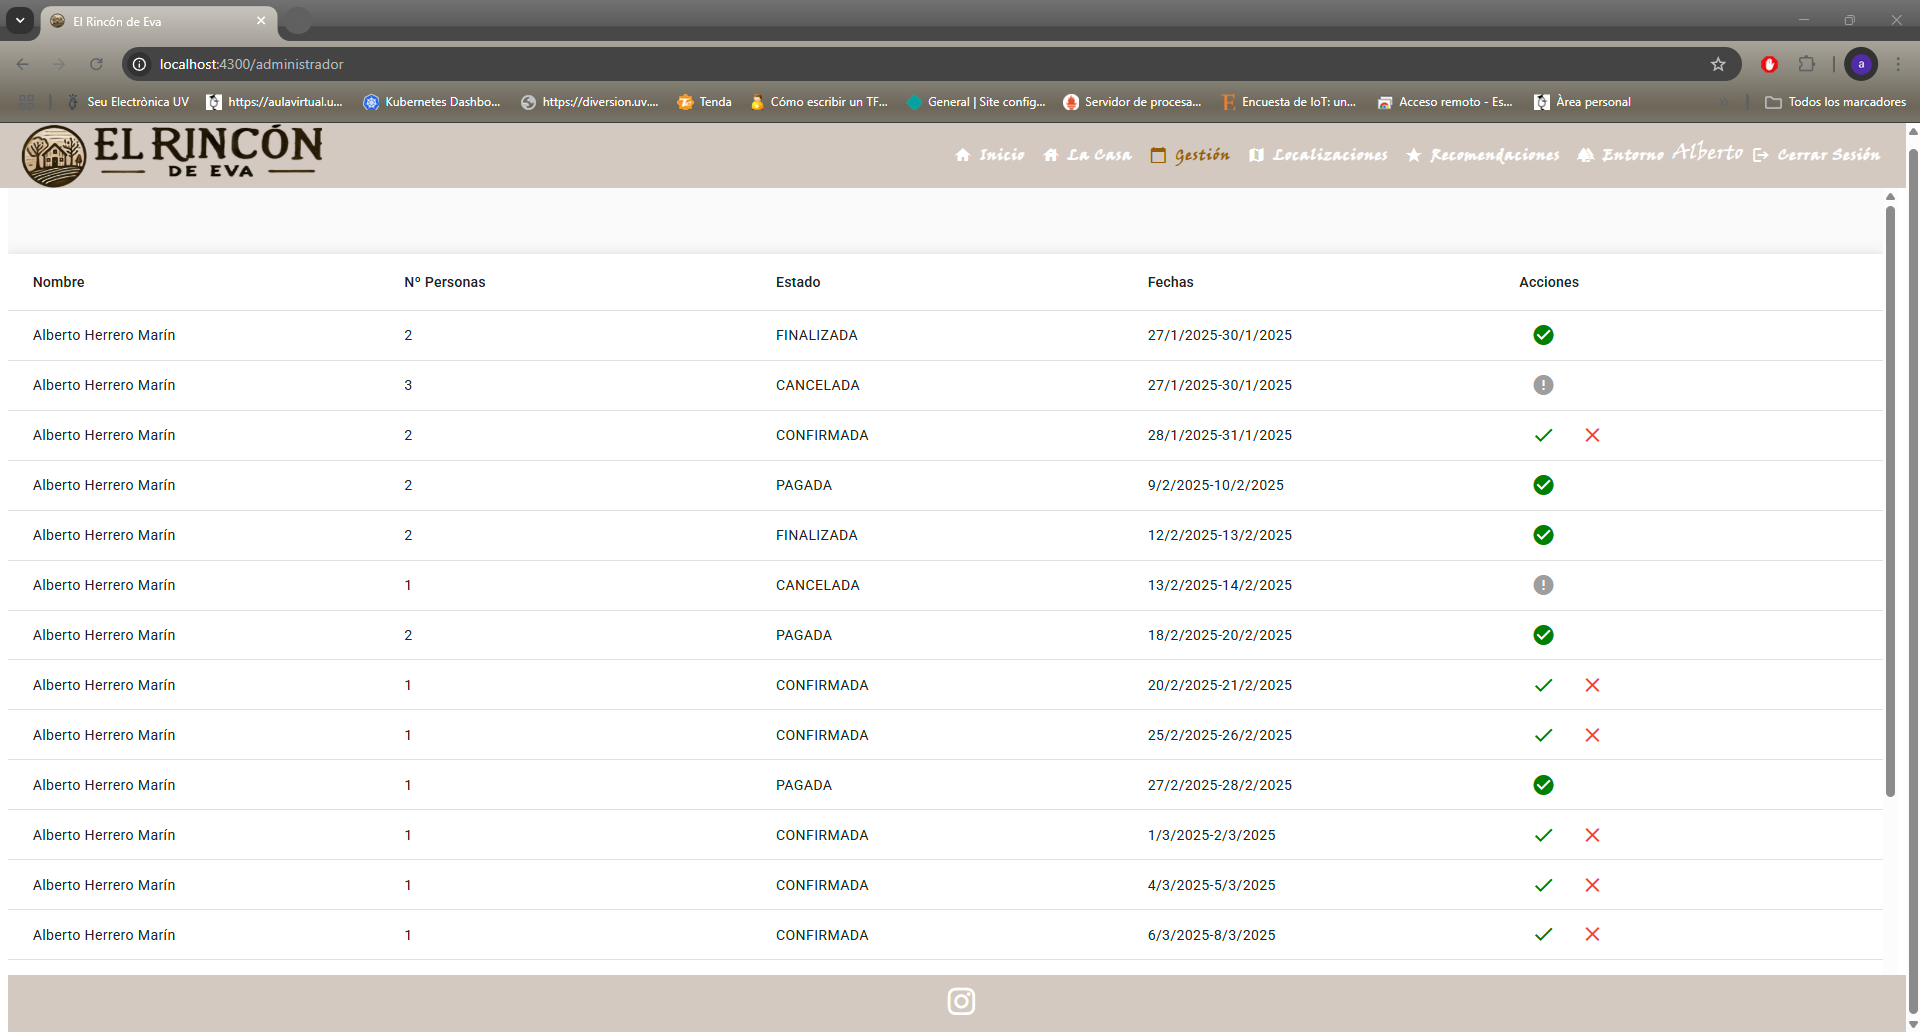
\includegraphics[width=1\textwidth]{figs/administrador.png}
    \caption{Diseño del componente \texttt{AdministradorComponent}}
    \label{fig:administrador_component}
\end{figure}

\subsubsection{Componente \texttt{InicioComponent}}

El componente \texttt{InicioComponent} gestiona la visualización de reseñas, la interacción del usuario con las reseñas (expandiéndolas y cargando más), así como el envío de reseñas y mensajes de contacto, con validación y manejo de errores.

La lógica de negocio se implementa en el archivo \texttt{inicio.component.ts}, donde destacan los métodos \texttt{onSubmitReview} y \texttt{onSubmit}. El método \texttt{onSubmitReview} se encarga de enviar una nueva reseña al backend, validando previamente el formulario de reseñas. Si la reseña es válida, se procesa y se envía al servicio \texttt{ReviewService}, mostrando un mensaje de confirmación al usuario mediante un \texttt{snackBar}. Después de enviar la reseña, se actualiza el estado de la sesión del usuario y se recargan las reseñas. Por otro lado, el método \texttt{onSubmit} maneja el envío de un formulario de contacto, validando los campos requeridos y, en caso de ser válido, enviando el mensaje al backend a través del \texttt{MailService}. Al igual que con las reseñas, si el contacto se envía correctamente, se muestra una notificación al usuario. Ambos métodos interactúan con el backend para actualizar la información, como puede verse en el Apéndice~\ref{ap:frontend-typescript}, Listado~\ref{lst:onSubmitReview}.
El archivo de plantilla \texttt{inicio.component.html} utiliza varios componentes de Angular Material para estructurar la interfaz, pero lo más relevante en cuanto a la interacción con el backend se encuentra en el manejo de reseñas y el formulario de contacto.

En la sección de reseñas, se emplea el \texttt{ngFor} para iterar sobre las reseñas disponibles en el backend. Para cada reseña, se muestra una calificación con estrellas utilizando el componente \texttt{mat-icon}, y los detalles adicionales de la reseña, como limpieza, ubicación y servicios, se cargan dinámicamente mediante la función \texttt{getStars()}. Las reseñas se obtienen a través de un servicio que consulta el backend, y la lógica de visualización de las mismas está implementada en el archivo \texttt{inicio.component.ts}. El usuario también puede cargar más reseñas mediante un botón que llama a la función \texttt{loadMoreReviews()}.

Además, el componente incluye un formulario para que los usuarios dejen sus reseñas. Este formulario está vinculado a un \texttt{formGroup} en el archivo \texttt{inicio.component.ts}, y su envío activa la función \texttt{onSubmitReview()}, que envía la información al backend para ser guardada. La validación del formulario se realiza de forma reactiva, asegurando que se cumplan los requisitos antes de permitir el envío.

En la sección de contacto, se incluye otro formulario que permite a los usuarios enviar un mensaje. Este formulario está también vinculado a un \texttt{formGroup} y, al ser enviado, ejecuta la función \texttt{onSubmit(contactForm)}, que se encarga de enviar los datos al backend para su procesamiento.

Estos componentes de Angular interactúan con el backend mediante servicios que gestionan las solicitudes HTTP y las respuestas correspondientes. La implementación detallada de estas interacciones puede consultarse en el Apéndice~\ref{ap:frontend-html}, Listado~\ref{lst:inicioComponentHtml}.

Para finalizar, en la Figura~\ref{fig:inicio-resenas-component} se muestra el diseño del apartado para revisar las reseñas existentes, en la Figura~\ref{fig:inicio-resenas-crear-component} se muestra como crearía un cliente reciente una nueva reseña (solo se muestra si la reserva del cliente ha finalizado y no ha dejado una reseña después de ésta) y en la Figura~\ref{fig:inicio-contacto-crear-component} se muestra el apartado para crear una consulta al propietario de la casa rural. En este último apartado, el cliente puede dejar su nombre, correo electrónico y mensaje, que serán enviados al propietario de la casa rural a través del servicio de correo electrónico implementado en el backend.
\begin{figure}[h!tb]
    \centering
    \includegraphics[width=1\textwidth]{figs/inicio_reseñas.png}
    \caption{Apartado para consultar reseñas existentes de \texttt{InicioComponent}}
    \label{fig:inicio-resenas-component}
\end{figure}

\begin{figure}[h!tb]
    \centering
    \includegraphics[width=1\textwidth]{figs/inicio_reseñas_cliente.png}
    \caption{Apartado con formulario para crear reseña de \texttt{InicioComponent}}
    \label{fig:inicio-resenas-crear-component}
\end{figure}

\begin{figure}[h!tb]
    \centering
    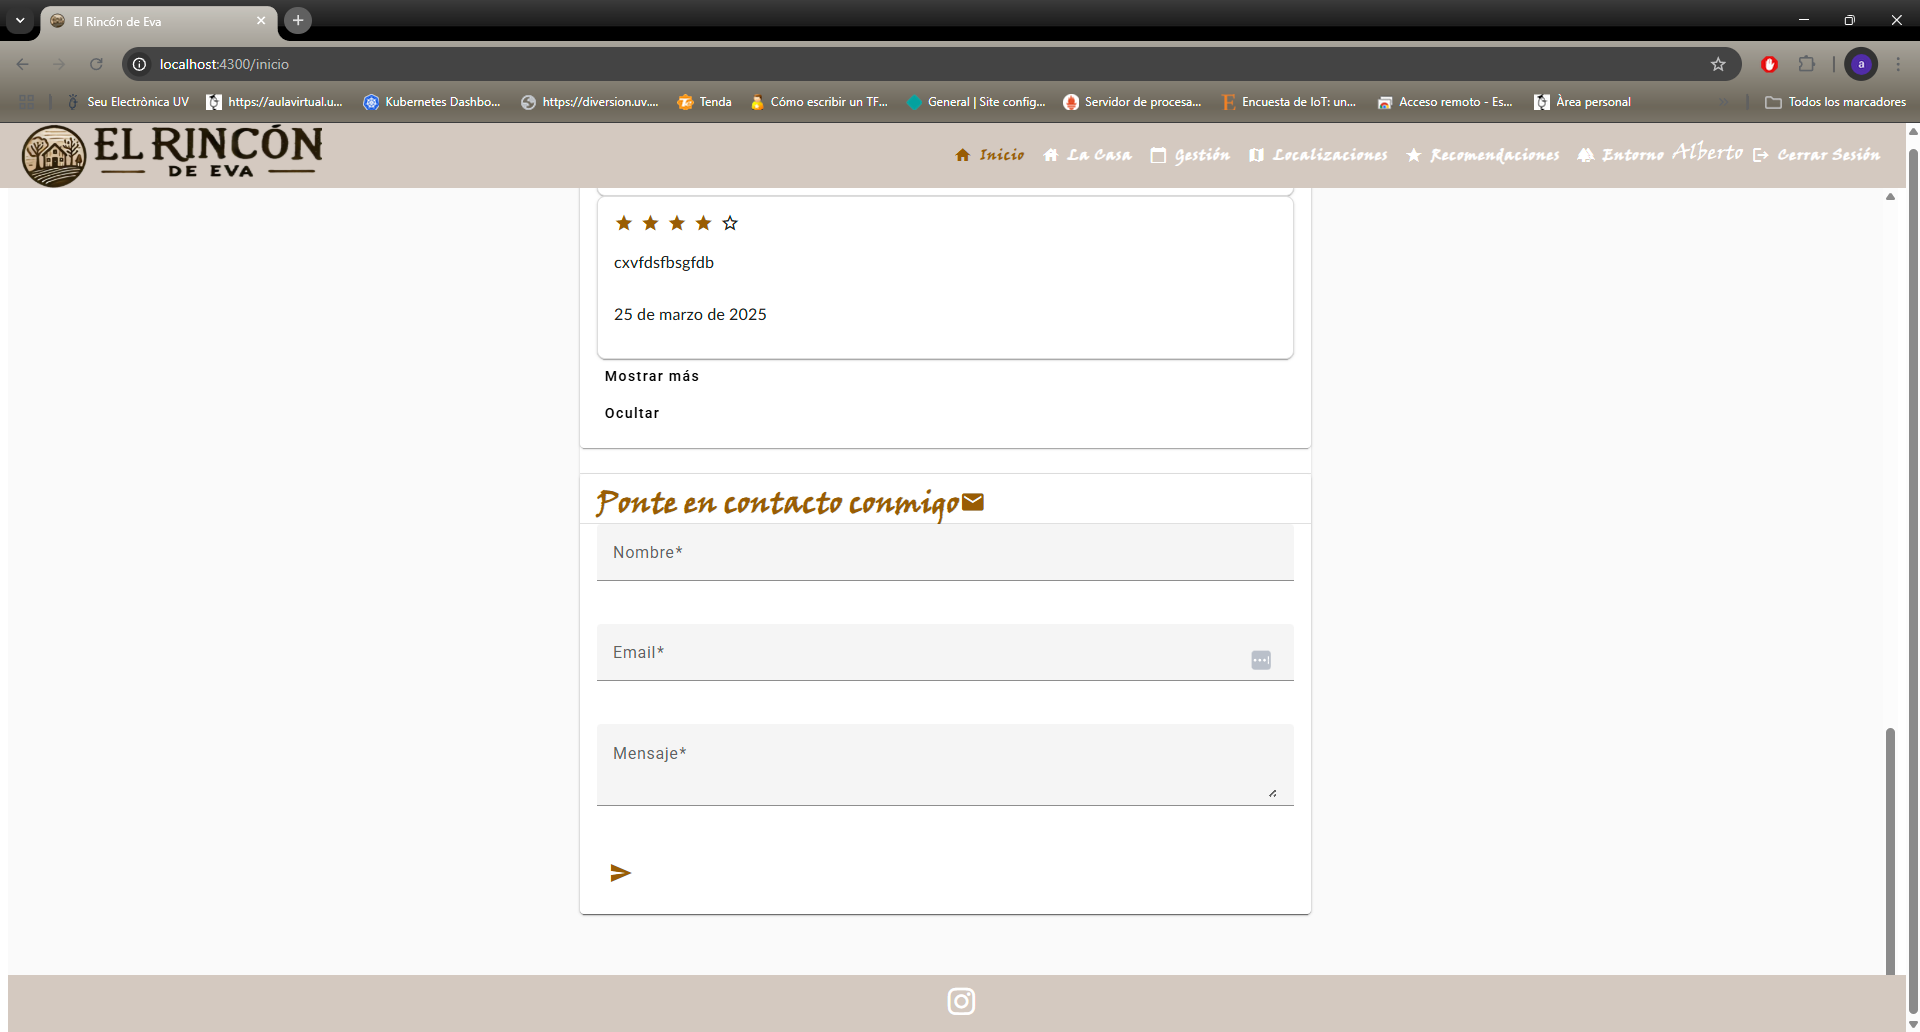
\includegraphics[width=1\textwidth]{figs/inicio_contacto.png}
    \caption{Apartado con formulario para crear una consulta de \texttt{InicioComponent}}
    \label{fig:inicio-contacto-crear-component}
\end{figure}

\subsubsection{Componente \texttt{LaCasaComponent}}

El componente \texttt{LaCasaComponent} gestiona la visualización de contenido multimedia relacionado con la casa rural. Su propósito es proporcionar una experiencia inmersiva a través de un video introductorio, un carrusel de imágenes que representan distintos espacios del alojamiento y una descripción textual detallada sobre las instalaciones, habitaciones y servicios ofrecidos.

La lógica de negocio se implementa en el archivo \texttt{la-casa.component.ts}, donde destacan los métodos \texttt{ngOnInit}, \texttt{fetchMedia}, \texttt{prevSlide} y \texttt{nextSlide}. En el método \texttt{ngOnInit} se inicializa la URL del video introductorio concatenando la base del backend con la ruta al recurso. Asimismo, se llama al método \texttt{fetchMedia()}, encargado de recuperar las imágenes del backend a través del servicio \texttt{MediaService}, que las devuelve como una colección de objetos \texttt{Media}. Estas imágenes se almacenan en el array \texttt{slides} para ser utilizadas en el carrusel.

Los métodos \texttt{prevSlide()} y \texttt{nextSlide()} permiten la navegación manual entre las imágenes del carrusel, modificando el índice \texttt{currentSlide} que controla qué conjunto de imágenes se muestra actualmente. El carrusel está configurado para mostrar dos imágenes por página, utilizando la constante \texttt{imagesPerSlide}.

El archivo de plantilla \texttt{la-casa.component.html} estructura la interfaz del usuario en varias secciones claramente diferenciadas. En primer lugar, se encuentra el video introductorio, que se obtiene dinámicamente desde el backend y se presenta con controles para su reproducción. A continuación, se encuentra el carrusel de imágenes, implementado con un contenedor que itera sobre \texttt{slides} utilizando \texttt{ngFor} y calcula el subconjunto de imágenes a mostrar en función de \texttt{currentSlide}.
La implementación detallada del componente puede consultarse en el Apéndice~\ref{ap:frontend-typescript}, Listado~\ref{lst:laCasaComponentTs}, mientras que la estructura \gls{html5} se encuentra en el Listado~\ref{lst:laCasaComponentHtml} del Apéndice~\ref{ap:frontend-html}.

En la Figura~\ref{fig:la-casa-carrusel-component} se muestra la sección del carrusel de imágenes (obtenidas de la integración de PublicacionesAPI) y el vídeo (obtenido del backend estático).

\begin{figure}[h!tb]
\centering
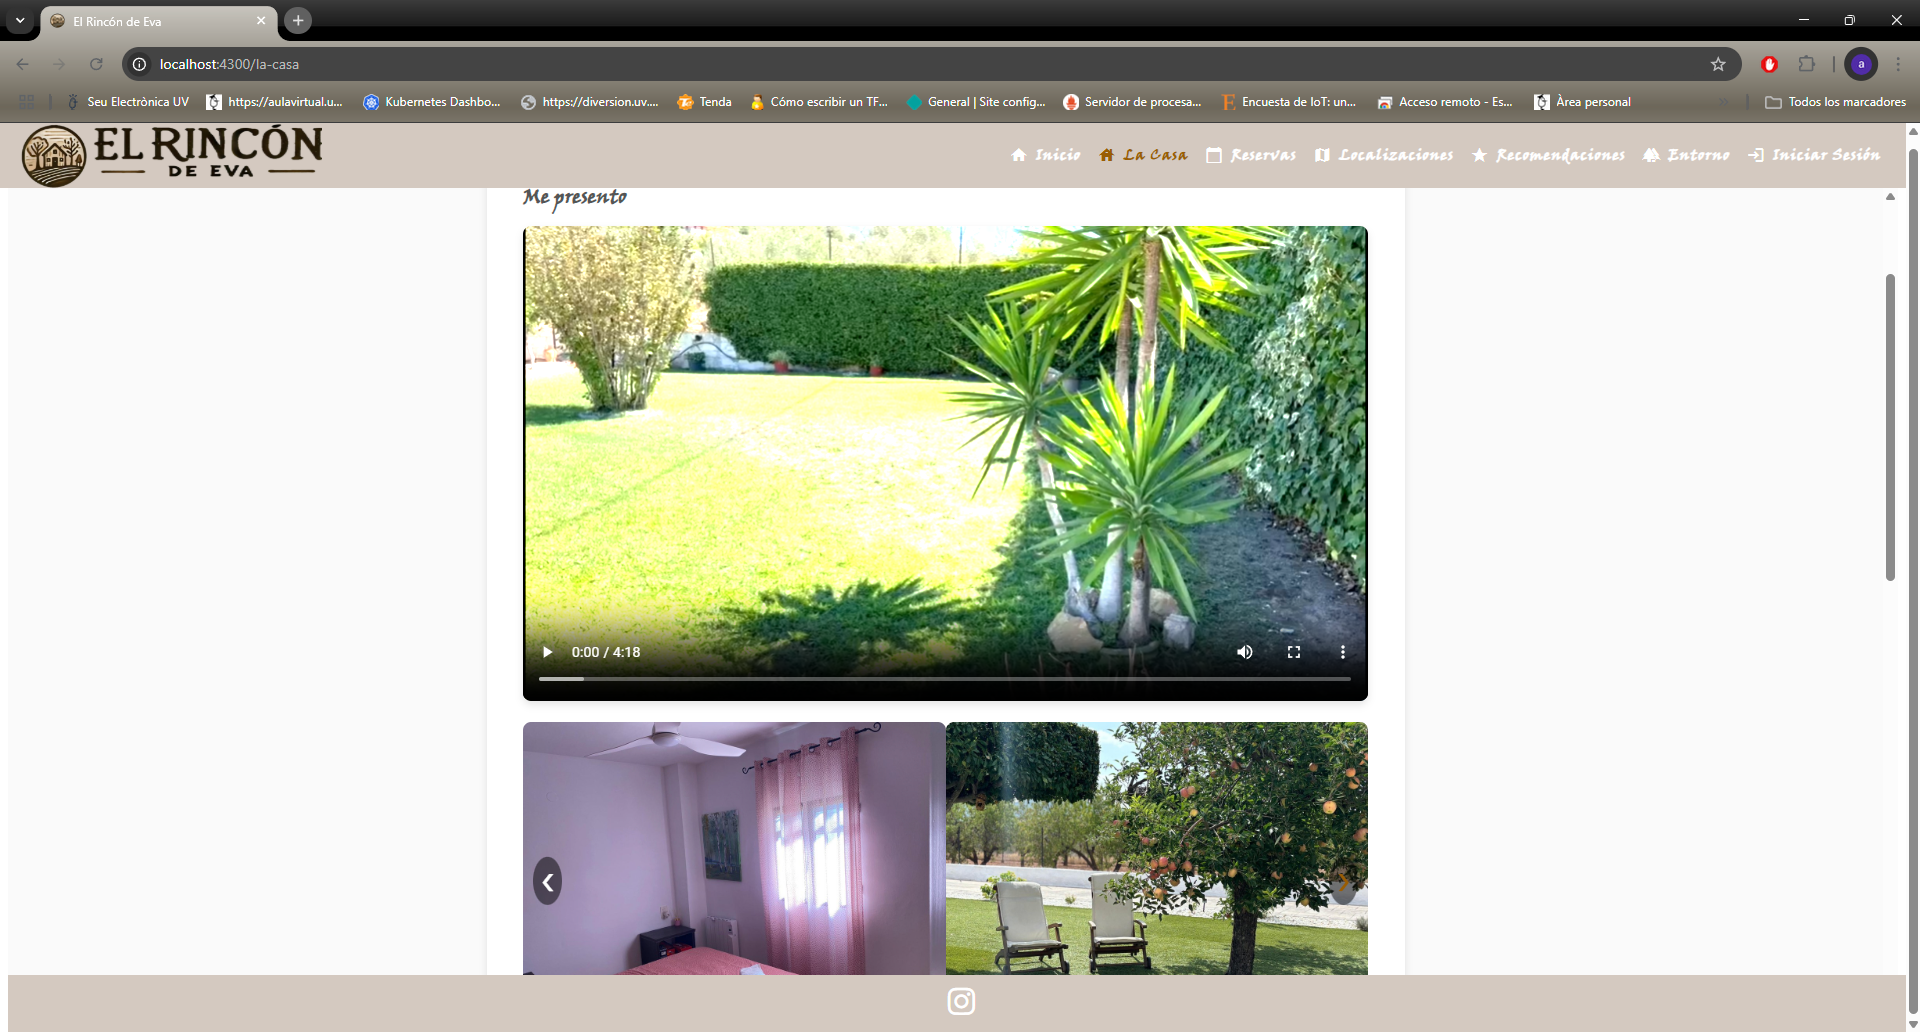
\includegraphics[width=1\textwidth]{figs/la_casa_carrusel.png}
\caption{Carrusel de imágenes en el componente \texttt{LaCasaComponent}}
\label{fig:la-casa-carrusel-component}
\end{figure}
\subsubsection{Componente \texttt{ReservaComponent}}
El componente \texttt{ReservaComponent} se encarga de gestionar todo el proceso de reserva de la casa rural. Para ello, se ha integrado un calendario interactivo mediante el componente \texttt{mwl-calendar-month-view}, cuya vista ha sido personalizada para adaptarse a los requisitos del negocio. En este calendario, los usuarios pueden visualizar las fechas ya reservadas, las cuales se cargan mediante el método \texttt{initializeEvents()}, que obtiene dicha información desde el servicio \texttt{reservaService}.

Además, el componente permite seleccionar rangos de fechas no reservadas. Una vez seleccionado un rango válido, se ejecuta el método \texttt{fetchWeather()}, que envía ese intervalo al \gls{backend} para obtener la previsión meteorológica de cada día del periodo. Esta información se encapsula en objetos \texttt{WeatherData}, los cuales se representan visualmente en un \texttt{MatCard} contiguo. Si el usuario hace clic sobre uno de los días seleccionados (marcados con un punto marrón), se invoca el método \texttt{onEventClicked()}, que despliega un formulario para completar los datos necesarios para la reserva, en caso de que no se puedan obtener directamente del usuario autenticado.

Una vez completado el formulario, se muestra un resumen de la reserva en un cuadro de diálogo (\texttt{MatDialog}), heredado del componente padre. Este resumen incluye el precio final calculado automáticamente en función de las tarifas aplicables. Si el usuario confirma, la reserva se envía de forma síncrona al \gls{backend} a través del servicio de reservas.

Adicionalmente, el componente permite consultar las reservas anteriores y futuras del usuario mediante una tabla. Esta tabla se alimenta de los datos proporcionados por el método \texttt{getReservasUser(email)} del servicio \texttt{reservaService}, y muestra entradas de tipo \texttt{Reserva}.

La implementación completa de este componente se detalla en el Apéndice~\ref{ap:frontend-typescript}, Listado~\ref{lst:reservasComponentTs}, mientras que su estructura \gls{html5} puede consultarse en el Listado~\ref{lst:reservasComponentHtml} del Apéndice~\ref{ap:frontend-html}.
En la Figura~\ref{fig:reservas-component} se muestra una vista completa del diseño de este componente. En la Figura~\ref{fig:reservas-resumen-component} se puede observar el cuadro de diálogo para finalizar la reserva el cual es generado por el componente \texttt{resumen-reserva.component}. 
    
\begin{figure}
    
    \centering
    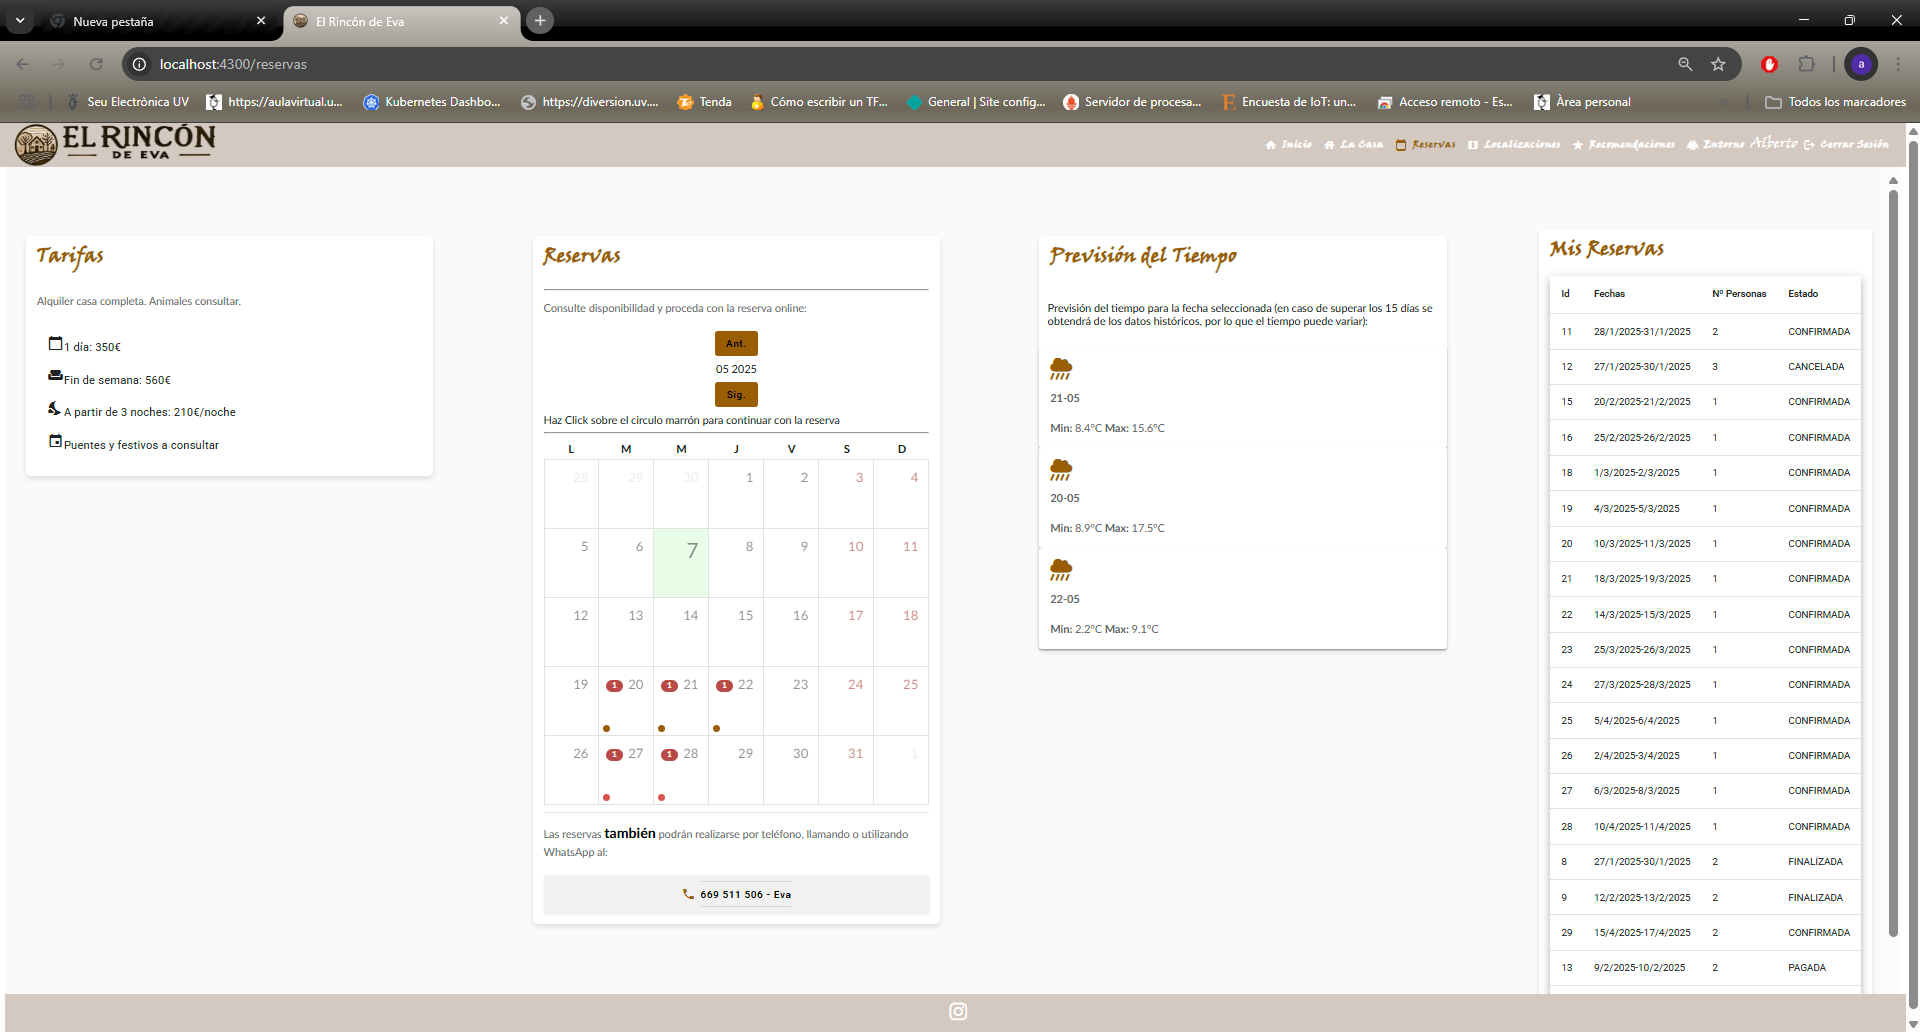
\includegraphics[width=1\textwidth]{figs/reservas.png}
    \caption{Vista general diseño del componente \texttt{ReservasComponent}}
    \label{fig:reservas-component}
\end{figure}

\begin{figure}

    \centering
        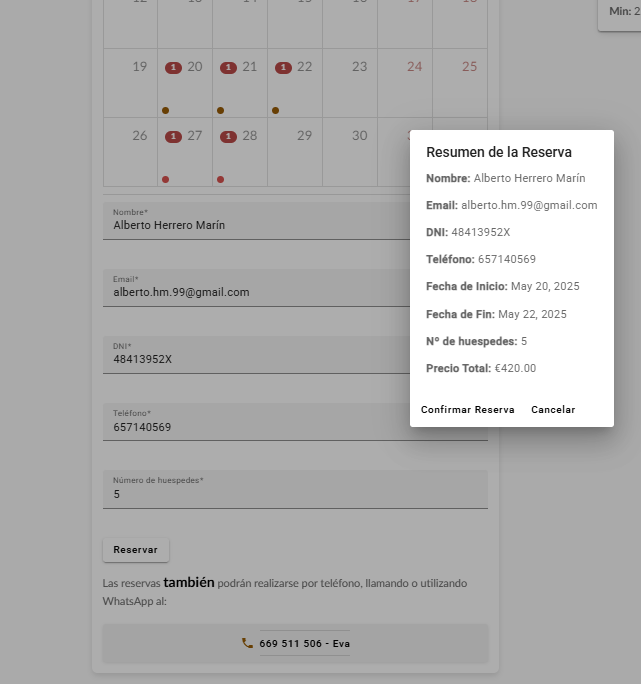
\includegraphics[width=0.6\textwidth]{figs/resumen-reserva.png}
        \caption{Vista del resúmen de la reserva en el componente \texttt{ReservasComponent}}
        \label{fig:reservas-resumen-component}
\end{figure}
\subsubsection{Componente \texttt{ComoLlegarComponent}}
El componente \texttt{ComoLlegarComponent} está diseñado para mostrar un mapa con la ubicación exacta de la casa rural, usando los mapas de Google. Además, muestra un mapa interactivo con rutas turísticas alrededor de la casa rural, aprovechando la biblioteca \texttt{Leaflet} y datos obtenidos mediante el servicio \texttt{OverpassService}, que utiliza la API de OpenStreetMap. Al inicializarse, se carga un mapa centrado en la ubicación de la casa rural, y se solicitan las rutas disponibles en la zona mediante el método \texttt{loadRoutes()}.

Este método procesa los elementos recibidos, almacenando los nodos en una caché interna mediante \texttt{filterNodes()}, y dibujando cada ruta como una polilínea sobre el mapa. Cada ruta es interactiva: al hacer clic sobre ella se ejecuta \texttt{showRouteDetails()}, que despliega un popup con opciones para visualizar la ruta en OpenStreetMap o descargarla en formato GPX. Esta descarga se genera dinámicamente mediante \texttt{downloadGPX()}, que transforma los datos de la ruta con el método \texttt{convertToGPX()}.

El mapa ajusta automáticamente el encuadre para mostrar todas las rutas encontradas, y permite una experiencia de navegación intuitiva y enriquecida para el usuario.


La implementación completa del componente puede consultarse en el Apéndice~\ref{ap:frontend-typescript}, Listado~\ref{lst:comoLlegarComponentTs}, mientras que su estructura \gls{html5} se encuentra en el Listado~\ref{lst:comoLlegarComponentHtml} del Apéndice~\ref{ap:frontend-html}.
En la Figura~\ref{fig:como-llegar-component} se muestra una vista completa del diseño de este componente.
\begin{figure}

    \centering
        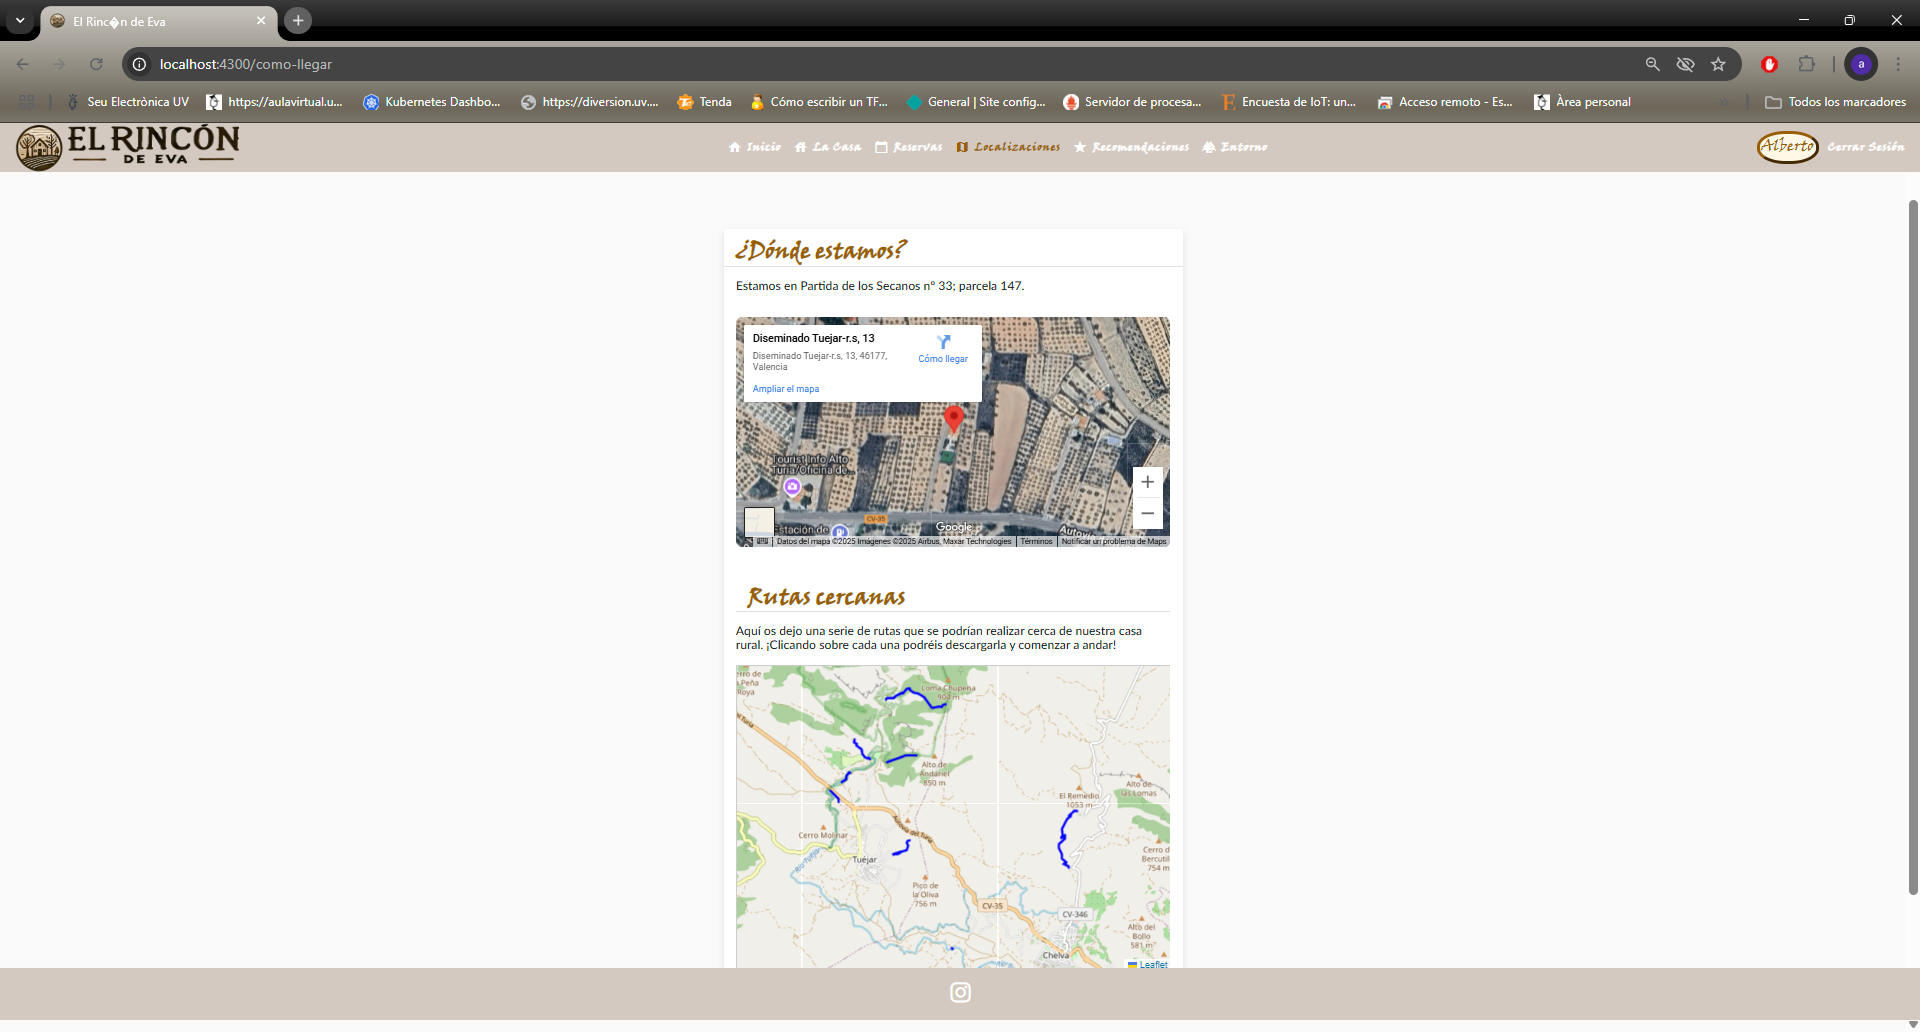
\includegraphics[width=1\textwidth]{figs/como-llegar.png}
        \caption{Vista del diseño del componente \texttt{ComoLlegarComponent}}
        \label{fig:como-llegar-component}
\end{figure}

\subsubsection{Componente \texttt{RecomendacionesComponent}}
El componente \texttt{RecomendacionesComponent} permite mostrar recomendaciones relacionadas con la gastronomía y las fiestas del entorno. En su inicialización, recupera listas de objetos de tipo \texttt{Entorno} y \texttt{Media} mediante los servicios \texttt{EntornoService} y \text{MediaService}, que se asigna al array \texttt{slidesFiestas} y \texttt{sledesComida} respectivamente.

El componente define dos carruseles: uno para imágenes de comida y otro para eventos festivos. La navegación entre imágenes se gestiona mediante métodos que actualizan los índices de desplazamiento de cada carrusel (\texttt{prevSlideComida()}, \texttt{nextSlideComida()}, \texttt{prevSlideFiesta()}, \texttt{nextSlideFiesta()}), mostrando los elementos en bloques de tres.

El código fuente se incluye en el Apéndice~\ref{ap:frontend-typescript}, Listado~\ref{lst:recomendacionesComponentTs}, y su correspondiente plantilla \gls{html5} puede consultarse en el Listado~\ref{lst:recomendacionesComponentHtml} del Apéndice~\ref{ap:frontend-html}.


En la Figura~\ref{fig:recomendaciones-component} se muestra una vista completa del diseño de este componente.
\begin{figure}

    \centering
        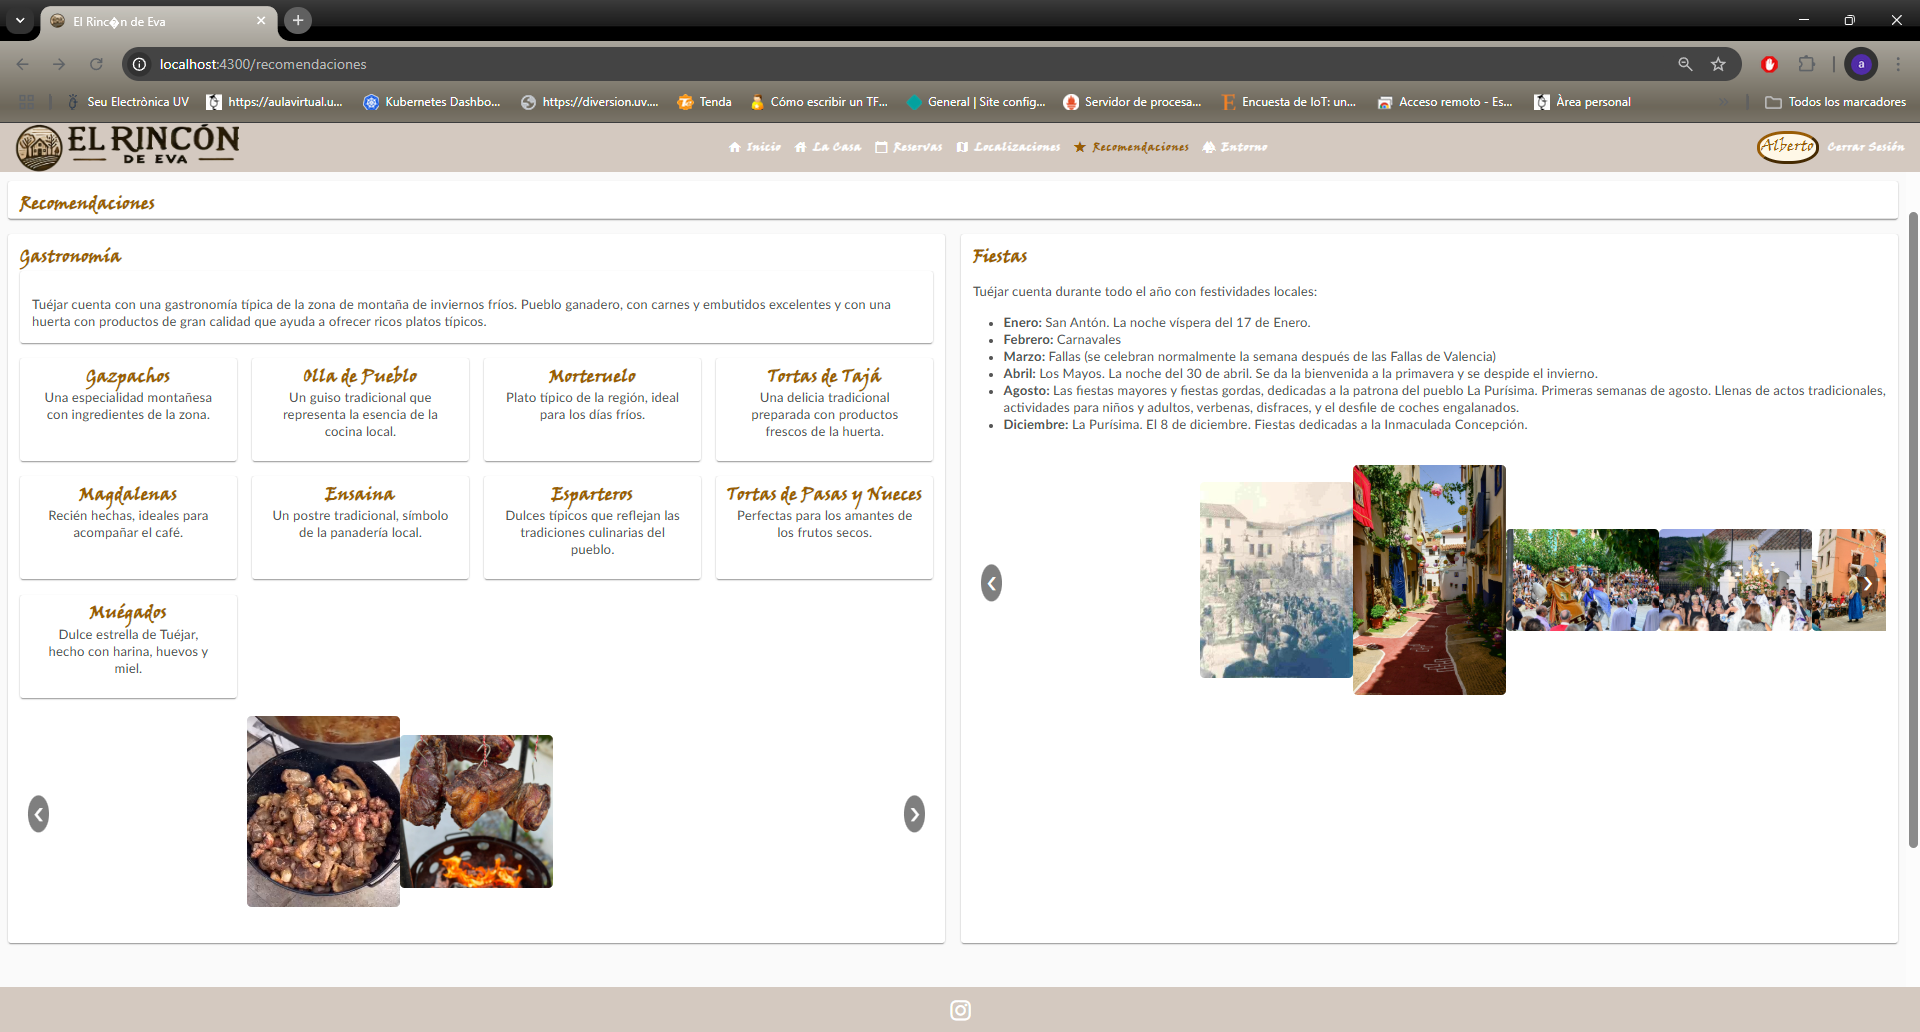
\includegraphics[width=1\textwidth]{figs/recomendaciones.png}
        \caption{Vista del diseño del componente \texttt{RecomendacionesComponent}}
        \label{fig:recomendaciones-component}
\end{figure}
\subsubsection{Componente \texttt{EntornoComponent}}
El componente \texttt{EntornoComponent} es responsable de mostrar los principales puntos de interés turístico de las localidades de Tuéjar y Chelva. Para ello, durante la inicialización se realiza una petición al backend mediante el servicio \texttt{EntornoService}, que obtiene un array de objetos \texttt{Entorno} a través del método \texttt{getEntorno()}. A partir de los datos obtenidos, se filtran dos subconjuntos diferenciados: uno para la localidad de Tuéjar y otro para Chelva, excluyendo en ambos casos los elementos cuya categoría corresponde a festividades.

Cada uno de estos subconjuntos se utiliza para poblar dinámicamente una sección distinta del componente, en la que se representa la información mediante tarjetas (\texttt{mat-card}) que muestran la imagen, título, descripción y un enlace al recurso externo asociado a cada lugar. La maquetación se presenta en formato de cuadrícula adaptable a través del uso de clases personalizadas.

La implementación detallada del componente puede consultarse en el Apéndice~\ref{ap:frontend-typescript}, Listado~\ref{lst:entornoComponentTs}, mientras que la estructura \gls{html5} se encuentra en el Listado~\ref{lst:entornoComponentHtml} del Apéndice~\ref{ap:frontend-html}.
En la Figura~\ref{fig:entorno-component} se muestra una vista completa del diseño de este componente.
\begin{figure}
    \centering
        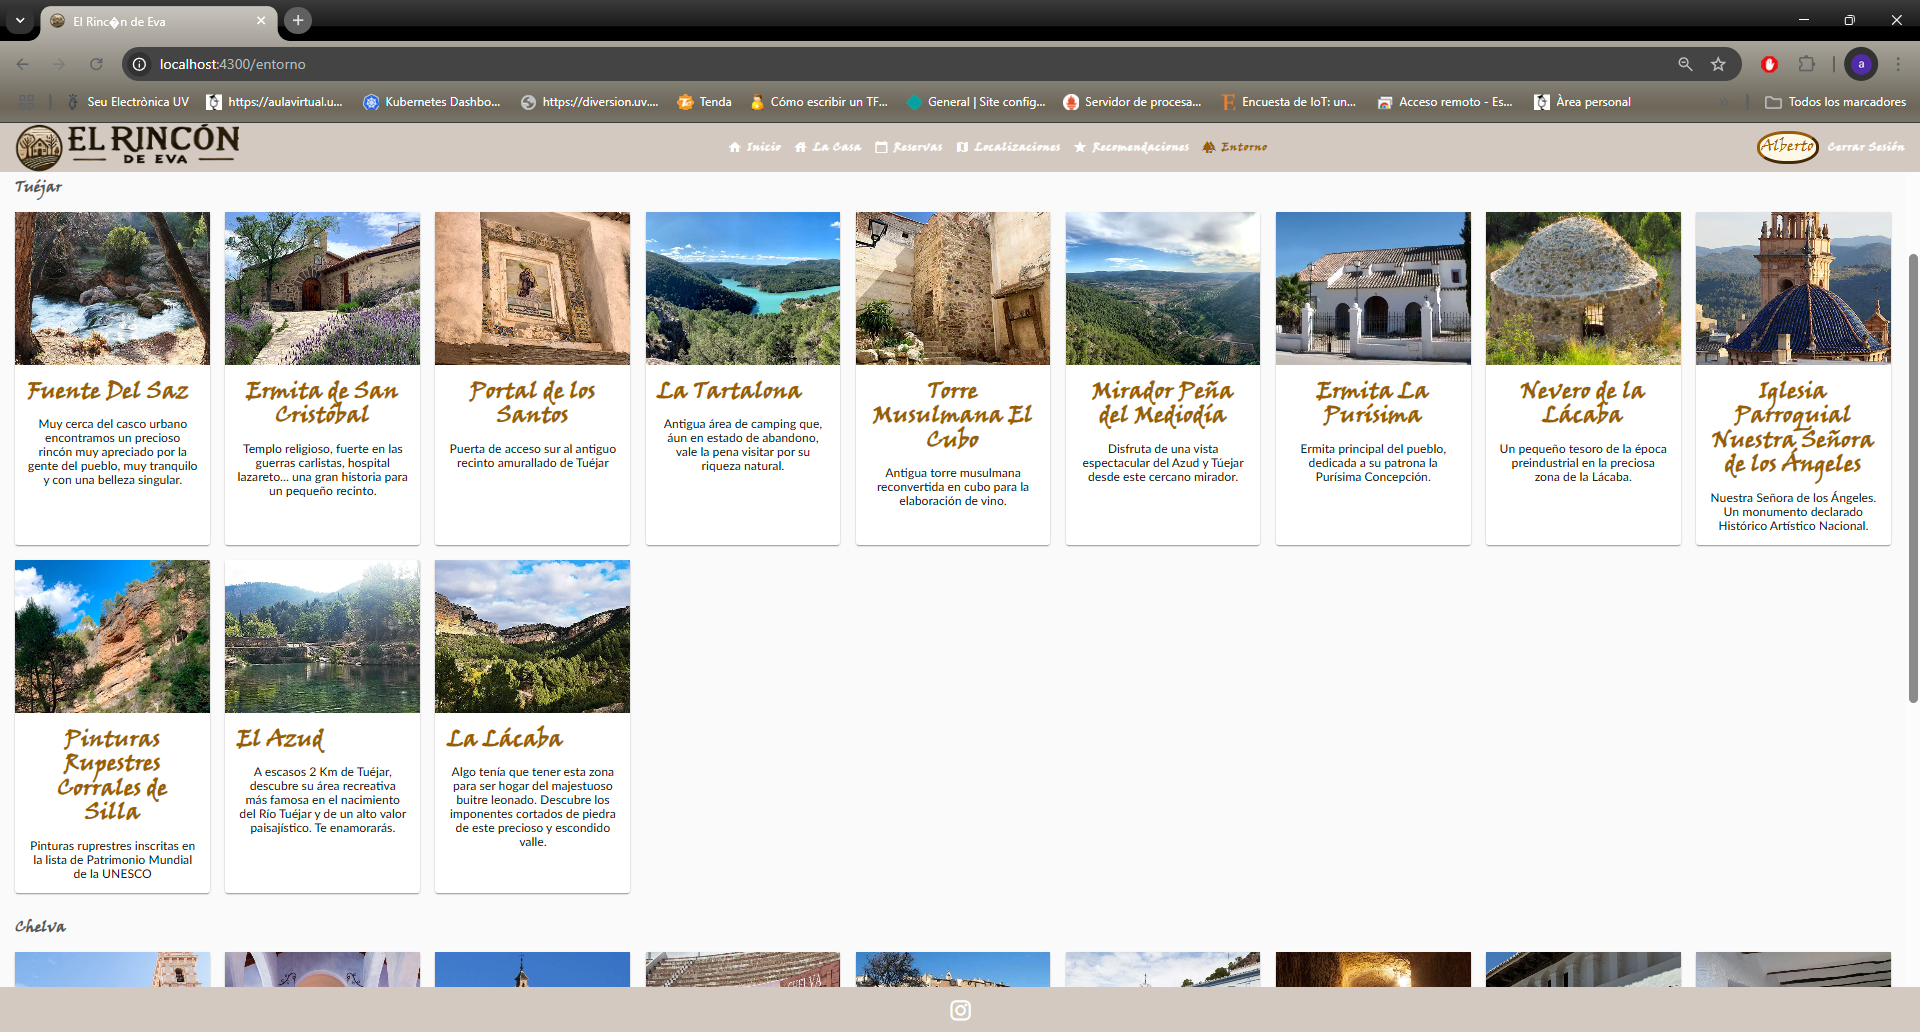
\includegraphics[width=1\textwidth]{figs/entorno.png}
        \caption{Vista del diseño del componente \texttt{EntornoComponent}}
        \label{fig:entorno-component}
\end{figure}
\section{Despliegue de aplicaciones basado en contenedores}
El despliegue de la aplicación basado en contenedores Docker se han llevado a cabo exclusivamente para la parte correspondiente al \gls{backend}. Para ello, se han generado previamente los archivos Dockerfile para cada una de las cuatro aplicaciones desarrolladas con \gls{springboot}.

En el Listado~\ref{lst:dockerfile} se presenta el Dockerfile correspondiente al servicio principal de la aplicación. En dicho archivo, se puede observar cómo se transfiere el paquete generado mediante la herramienta Maven~\cite{maven:web}, a través del comando \texttt{mvn clean package}, al entorno de ejecución definido en Docker. Posteriormente, se procede a la ejecución del archivo \texttt{.jar} utilizando el perfil denominado \texttt{despliegue}, el cual ha sido configurado con variables de entorno específicas en el entorno \gls{springboot}. Estas variables serán sobreescritas posteriormente mediante los archivos de configuración utilizados en los despliegues de \gls{kubernetes}.

Los restantes Dockerfile presentan una estructura similar, diferenciándose únicamente en el nombre de la aplicación correspondiente. Para mayor detalle, en el Apéndice~\ref{ap:docker} se incluyen los Dockerfile de las otras tres aplicaciones del sistema.
\begin{longlisting}
\caption{Dockerfile del servicio de la aplicación principal {\tt Dockerfile}}
\inputminted{docker}{../backend/despliegue/elrincondeeva/Dockerfile}
\label{lst:dockerfile}
\end{longlisting}

Posteriormente, estas imágenes se han subido a un registro privado de Docker, donde se encuentran disponibles para su despliegue en el clúster de \gls{kubernetes} del entorno de producción. 

A continuación, se describen cada uno de los elementos que componen el despliegue de la aplicación en el clúster de \gls{kubernetes}, los cuales se han generado mediante ficheros \gls{yaml}:

\subsection{Almacenamiento Persistente: \gls{pv} y \gls{pvc}}

\begin{itemize}
  \item \textbf{PostgreSQL}:
  \begin{itemize}
    \item Se define un volumen persistente \texttt{postgres-pv}, Listado~\ref{lst:pv-postgres}, para el almacenamiento de datos de la base de datos.
    \item El volumen se reclama mediante \texttt{postgres-pvc}, Listado~\ref{lst:pvc-postgres}.
  \end{itemize}

  \begin{longlisting}
  \caption{PersistentVolume de PostgreSQL}
  \inputminted[firstline=5,lastline=15]{yaml}{../backend/despliegue/kubernetes/despliegue.yaml}
  \label{lst:pv-postgres}
  \end{longlisting}

  \begin{longlisting}
  \caption{PersistentVolumeClaim de PostgreSQL}
  \inputminted[firstline=17,lastline=26]{yaml}{../backend/despliegue/kubernetes/despliegue.yaml}
  \label{lst:pvc-postgres}
  \end{longlisting}

  \item \textbf{MongoDB}:
  \begin{itemize}
    \item Se declara el volumen persistente \texttt{mongo-pv}, Listado~\ref{lst:pv-mongo}.
    \item Se reclama con \texttt{mongo-pvc}, Listado~\ref{lst:pvc-mongo}, para uso compartido por varias aplicaciones.
  \end{itemize}

  \begin{longlisting}
  \caption{PersistentVolume de MongoDB}
  \inputminted[firstline=30,lastline=40]{yaml}{../backend/despliegue/kubernetes/despliegue.yaml}
  \label{lst:pv-mongo}
  \end{longlisting}

  \begin{longlisting}
  \caption{PersistentVolumeClaim de MongoDB}
  \inputminted[firstline=42,lastline=51]{yaml}{../backend/despliegue/kubernetes/despliegue.yaml}
  \label{lst:pvc-mongo}
  \end{longlisting}

  \item \textbf{Token de Instagram (publicacionesapi)}:
  \begin{itemize}
    \item Volumen \texttt{token-pv}, Listado~\ref{lst:pv-token}, para almacenar el fichero \texttt{token.txt}.
    \item \gls{pvc} asociado: \texttt{token-pvc}, Listado~\ref{lst:pvc-token}.
  \end{itemize}

  \begin{longlisting}
  \caption{PersistentVolume del token de Instagram}
  \inputminted[firstline=55,lastline=65]{yaml}{../backend/despliegue/kubernetes/despliegue.yaml}
  \label{lst:pv-token}
  \end{longlisting}

  \begin{longlisting}
  \caption{PersistentVolumeClaim del token de Instagram}
  \inputminted[firstline=69,lastline=78]{yaml}{../backend/despliegue/kubernetes/despliegue.yaml}
  \label{lst:pvc-token}
  \end{longlisting}
\end{itemize}

\subsection{Despliegues y Servicios de las Aplicaciones y Bases de Datos}
El despliegue de las aplicaciones y bases de datos se realiza mediante recursos de tipo \texttt{Deployment} y \texttt{Service}. A continuación, se describen los elementos más relevantes de cada uno de ellos.
\subsection*{Componentes del Despliegue en Kubernetes}

\subsubsection*{PostgreSQL}
\begin{itemize}
  \item El \textbf{Deployment de PostgreSQL}, Listado~\ref{lst:postgres-deployment}, define:
  \begin{itemize}
    \item Una única réplica del contenedor con la imagen oficial de \texttt{postgres:17}.
    \item Variables de entorno para configurar el nombre de la base de datos, usuario y contraseña.
    \item Montaje de un volumen persistente a \texttt{/var/lib/postgresql/data}, usando el \texttt{PersistentVolumeClaim} llamado \texttt{postgres-pvc}.
  \end{itemize}
  \begin{longlisting}
\caption{Deployment de PostgreSQL}
\inputminted[firstline=84,lastline=116]{yaml}{../backend/despliegue/kubernetes/despliegue.yaml}
\label{lst:postgres-deployment}
\end{longlisting}
  \item El \textbf{Service de PostgreSQL}, Listado~\ref{lst:postgres-service}, permite el acceso interno al contenedor:
  \begin{itemize}
    \item Expone el puerto \gls{tcp} \texttt{5432}.
    \item Usa \texttt{clusterIP: None} para permitir la detección por \gls{dns} entre pods.
  \end{itemize}
\end{itemize}

\begin{longlisting}
\caption{Service de PostgreSQL}
\inputminted[firstline=118,lastline=129]{yaml}{../backend/despliegue/kubernetes/despliegue.yaml}
\label{lst:postgres-service}
\end{longlisting}


\subsubsection*{MongoDB}
\begin{itemize}
  \item El \textbf{Deployment de MongoDB}, Listado~\ref{lst:mongo-deployment}, configura:
  \begin{itemize}
    \item Un pod basado en la imagen oficial \texttt{mongo:8}.
    \item Montaje de volumen persistente para los datos en \texttt{/data/db}, enlazado a \texttt{mongo-pvc}.
  \end{itemize}

  \begin{longlisting}
\caption{Deployment de MongoDB}
\inputminted[firstline=133,lastline=158]{yaml}{../backend/despliegue/kubernetes/despliegue.yaml}
\label{lst:mongo-deployment}
\end{longlisting}

  \item El \textbf{Service de MongoDB}, Listado~\ref{lst:mongo-service}, facilita el acceso interno:
  \begin{itemize}
    \item Expone el puerto estándar \texttt{27017}.
    \item Usa \texttt{clusterIP: None}, como el caso de \gls{postgresql}.
  \end{itemize}
\end{itemize}



\begin{longlisting}
\caption{Service de MongoDB}
\inputminted[firstline=160,lastline=170]{yaml}{../backend/despliegue/kubernetes/despliegue.yaml}
\label{lst:mongo-service}
\end{longlisting}


\subsubsection*{Aplicación ElRinconDeEva}
\begin{itemize}
  \item El \textbf{Deployment de ElRinconDeEva}, que se detalla en el Listado~\ref{lst:elrincondeeva-deployment}, incluye:
  \begin{itemize}
    \item Una aplicación Spring Boot contenida en la imagen \texttt{albherre/elrincondeeva-app:v3}.
    \item Variables de entorno para definir las URLs de conexión a servicios como \gls{postgresql}, \texttt{publicacionesapi}, \texttt{tiempo} y \texttt{extracción}.
    \item Un contenedor de inicialización (\texttt{initContainer}) que espera a que \gls{postgresql} esté disponible antes de iniciar la aplicación principal.
  \end{itemize}
  \begin{longlisting}
\caption{Deployment de ElRinconDeEva}
\inputminted[firstline=176,lastline=216]{yaml}{../backend/despliegue/kubernetes/despliegue.yaml}
\label{lst:elrincondeeva-deployment}
\end{longlisting}
  \item El \textbf{Service de ElRinconDeEva}, que se detalla en el Listado~\ref{lst:elrincondeeva-service}, permite la comunicación interna y externa:
  \begin{itemize}
    \item Redirige el tráfico del puerto \texttt{80} al \texttt{8080} del contenedor.
    \item Usa tipo \texttt{LoadBalancer} por defecto para comunicar con el exterior por medio del Ingress.
  \end{itemize}
\end{itemize}

\begin{longlisting}
\caption{Service de ElRinconDeEva}
\inputminted[firstline=219,lastline=229]{yaml}{../backend/despliegue/kubernetes/despliegue.yaml}
\label{lst:elrincondeeva-service}
\end{longlisting}

\subsubsection*{publicacionesapi}
\begin{itemize}
  \item El \textbf{Deployment de publicacionesapi}, que se detalla en el Listado~\ref{lst:publicacionesapi-deployment}, contiene:
  \begin{itemize}
    \item Una aplicación Spring Boot con la imagen \texttt{albherre/publicacionesapi-app:v2}.
    \item Uso de \texttt{initContainers} para:
      \begin{itemize}
        \item Esperar a que \gls{mongodb} esté disponible.
        \item Crear un archivo \texttt{token.txt} en un volumen persistente si no existe.
      \end{itemize}
    \item Montaje de un volumen persistente desde \texttt{token-pvc}.
  \end{itemize}
  \begin{longlisting}
\caption{Deployment de publicacionesapi}
\inputminted[firstline=233,lastline=284]{yaml}{../backend/despliegue/kubernetes/despliegue.yaml}
\label{lst:publicacionesapi-deployment}
\end{longlisting}


  \item El \textbf{Service de publicacionesapi}, que se detalla en el Listado~\ref{lst:publicacionesapi-service}, proporciona acceso interno:
  \begin{itemize}
    \item Redirige el puerto estándar \texttt{8080}.
  \end{itemize}
\end{itemize}

\begin{longlisting}
\caption{Service de publicacionesapi}
\inputminted[firstline=288,lastline=298,fontsize=\small, breaklines, breakanywhere]{yaml}{../backend/despliegue/kubernetes/despliegue.yaml}
\label{lst:publicacionesapi-service}
\end{longlisting}

\subsubsection*{tiempo}
\begin{itemize}
  \item El \textbf{Deployment de tiempo}, que se detalla en el Listado~\ref{lst:tiempo-deployment}, define:
  \begin{itemize}
    \item El contenedor de la aplicación meteorológica, expuesto en el puerto \texttt{8080}.
    \item Uso de \texttt{initContainers} para esperar a que \gls{mongodb} esté disponible.
    \item Variables de entorno de conexión al servicio \gls{mongodb} para almacenamiento de datos meteorológicos.
  \end{itemize}
  \begin{longlisting}
\caption{Deployment de tiempo}
\inputminted[firstline=302,lastline=330]{yaml}{../backend/despliegue/kubernetes/despliegue.yaml}
\label{lst:tiempo-deployment}
\end{longlisting}
  \item El \textbf{Service de tiempo}, que se detalla en el Listado~\ref{lst:tiempo-service}, habilita el acceso interno entre pods:
  \begin{itemize}
    \item Enruta tráfico al puerto \texttt{8080}.
  \end{itemize}
\end{itemize}



\begin{longlisting}
\caption{Service de tiempo}
\inputminted[firstline=332,lastline=342]{yaml}{../backend/despliegue/kubernetes/despliegue.yaml}
\label{lst:tiempo-service}
\end{longlisting}

\subsubsection*{extraccion}
\begin{itemize}
  \item El \textbf{Deployment de extraccion}, que se detalla en el Listado~\ref{lst:extraccion-deployment}, contiene:
  \begin{itemize}
    \item El contenedor de la aplicación que realiza tareas de scraping y transformación de datos.
    \item Uso de \texttt{initContainers} para esperar a que \gls{mongodb} esté disponible.
    \item Variables de entorno para conexión con \gls{mongodb} para almacenar resultados extraídos.
  \end{itemize}
  \begin{longlisting}
\caption{Deployment de extraccion}
\inputminted[firstline=346,lastline=374]{yaml}{../backend/despliegue/kubernetes/despliegue.yaml}
\label{lst:extraccion-deployment}
\end{longlisting}
  \item El \textbf{Service de extraccion}, que se detalla en el Listado~\ref{lst:extraccion-service}, configura su exposición:
  \begin{itemize}
    \item Utiliza el puerto \texttt{8080}.
  \end{itemize}
\end{itemize}

\begin{longlisting}
\caption{Service de extraccion}
\inputminted[firstline=376,lastline=386]{yaml}{../backend/despliegue/kubernetes/despliegue.yaml}
\label{lst:extraccion-service}
\end{longlisting}

\subsection{Ingress Controller}

\begin{itemize}
  \item Se define un recurso de tipo \texttt{Ingress}, Listado~\ref{lst:ingress}, que enruta el tráfico \gls{https} hacia el servicio principal.
  \item Se utiliza \gls{tls} a través de un \texttt{secret} denominado \texttt{elrincondeeva-tls}, asi se prepara para su despliegue en la nube en un futuro.
  \item La ruta principal redirige al servicio \texttt{elrincondeeva}.
\end{itemize}

\begin{longlisting}
\caption{Recurso Ingress para el acceso HTTPS}
\inputminted[firstline=390,lastline=411]{yaml}{../backend/despliegue/kubernetes/despliegue.yaml}
\label{lst:ingress}
\end{longlisting}

Una vez desplegada la infraestructura se comprueba graficamente mediante el panel de control de \gls{kubernetes} que todos los pods se encuentran en estado \texttt{Running} y que los servicios están correctamente configurados. En la Figura~\ref{fig:kubernetes-dashboard} se muestra una captura de pantalla del panel de control de \gls{kubernetes} donde se puede observar el estado de los pods y servicios desplegados.
\begin{figure}[h!tb]
    \centering
    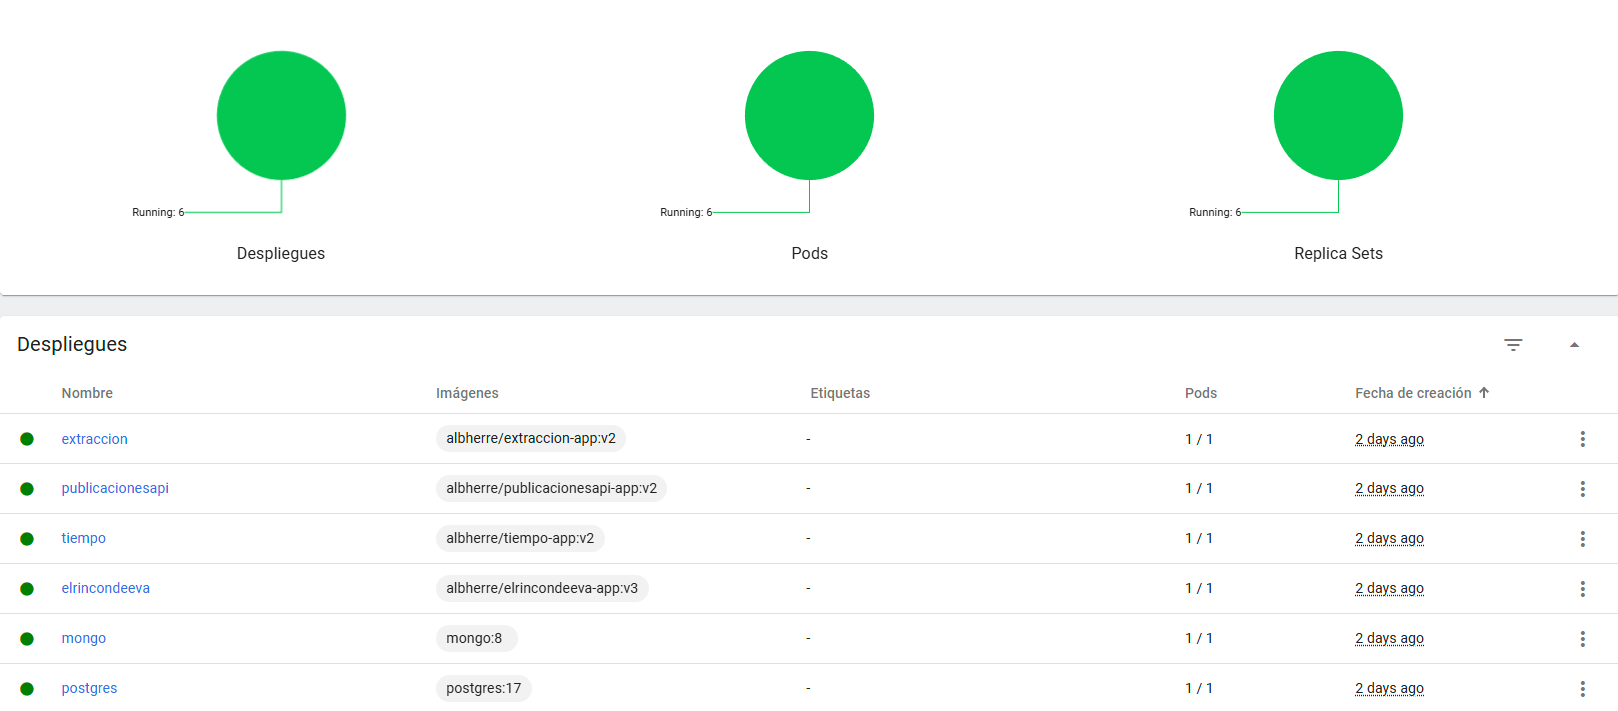
\includegraphics[width=1\textwidth]{figs/kubernetes-dashboard.png}
    \caption{Panel de control de Kubernetes mostrando el estado de los pods y servicios}\label{fig:kubernetes-dashboard}
\end{figure}


\clearpage
\section{Pruebas}
\subsection{Pruebas unitarias de la aplicación web}
Estas pruebas se han realizado exclusivamente en la parte del \gls{backend} de la aplicación, se ha utilizado Postman~\cite{postman:web} para realizar llamadas a cada uno de los endpoints generados y validar su funcionamiento y se ha utilizado las herramientas JUnit~\cite{junit:web} y Mockito~\cite{mockito:web} para la ejecución de pruebas unitarias sobre algunos de los servicios más relevantes y cuya lógica es mas compleja dentro de la aplicación. A continuación se describen las pruebas más relevantes realizadas en el \gls{backend} de la aplicación:
\begin{itemize}
    \item \textbf{Pruebas de servicios de reservas}: Se han creado pruebas para verificar que los servicios de reservas funcionan correctamente, incluyendo la creación y modificación de reservas. En el Apéndice~\ref{ap:test}, Listado~\ref{lst:reservaServiceTest}, se puede consultar el código fuente de las pruebas unitarias realizadas en el servicio de reservas.
     \begin{itemize}
      \item \textbf{testConfirmarReserva\_usuarioExiste\_reservaConfirmada}
        \begin{itemize}
          \item Simula el caso en que el usuario ya existe en el sistema.
          \item Crea una reserva y la guarda correctamente.
          \item Verifica que se envía un correo de confirmación.
          \item Comprueba que el ID devuelto por la reserva es el esperado.
        \end{itemize}

      \item \textbf{testConfirmarReserva\_usuarioNoExiste\_lanzaExcepcion}
        \begin{itemize}
          \item Simula el caso en que el usuario no existe en el sistema.
          \item Verifica que se lanza una excepción con el mensaje ``Usuario no encontrado''.
        \end{itemize}

      \item \textbf{testConfirmarPagoReserva\_enviaEmail}
        \begin{itemize}
          \item Simula la confirmación del pago de una reserva existente.
          \item Verifica que se recupera correctamente la reserva por ID.
          \item Comprueba que se envía un correo de confirmación del pago.
        \end{itemize}

      \item \textbf{testCancelarReserva\_enviaEmail}
        \begin{itemize}
          \item Simula la cancelación de una reserva existente.
          \item Verifica que se recupera correctamente la reserva por ID.
          \item Comprueba que se envía un correo de cancelación con el motivo indicado.
        \end{itemize}
    \end{itemize}
    \item \textbf{Pruebas de servicios de usuarios}: Se han diseñado pruebas para verificar que los servicios de gestión de usuarios funcionan correctamente, incluyendo el registro, inicio de sesión y recuperación de contraseñas. En el Apéndice~\ref{ap:test}, Listado~\ref{lst:userServiceTest} y Listado~\ref{lst:signupServiceTest} se puede consultar el código fuente de las pruebas unitarias realizadas en el servicio de usuario.
       \begin{itemize}
        \item \textbf{testGetNombre\_usuarioExistente}
          \begin{itemize}
            \item Simula la existencia de un usuario con un correo electrónico dado.
            \item Verifica que se devuelve correctamente el objeto \texttt{MyUser} correspondiente.
            \item Comprueba que el email del usuario es el esperado.
          \end{itemize}

        \item \textbf{testGetNombre\_usuarioNoExiste}
          \begin{itemize}
            \item Simula la ausencia de un usuario con el correo electrónico indicado.
            \item Verifica que se devuelve \texttt{null}.
          \end{itemize}

        \item \textbf{testGetRoles\_retornaRolesCorrectamente}
          \begin{itemize}
            \item Simula un usuario con dos roles asociados.
            \item Verifica que se recuperan correctamente los roles del usuario mediante sus identificadores.
            \item Comprueba que se devuelven los nombres de roles esperados: \texttt{ROLE\_USER} y \texttt{ROLE\_ADMIN}.
          \end{itemize}

        \item \textbf{testGetRoles\_usuarioNoExiste}
          \begin{itemize}
            \item Simula que el usuario no existe en la base de datos.
            \item Verifica que la lista de roles devuelta es vacía.
          \end{itemize}
        \item \textbf{testRegisterUser\_emailYaRegistrado\_lanzaExcepcion}
          \begin{itemize}
            \item Simula que el correo electrónico ya está registrado.
            \item Verifica que se lanza una excepción con un mensaje indicando que el email ya está en uso.
          \end{itemize}

        \item \textbf{testRegisterUser\_nuevoUsuario\_guardadoCorrectamente}
          \begin{itemize}
            \item Simula el registro de un nuevo usuario con datos válidos.
            \item Verifica que se encripta la contraseña, se guarda el usuario y se le asigna el rol \texttt{ROLE\_USER}.
            \item Confirma que el resultado no es nulo.
          \end{itemize}

        \item \textbf{testRegisterAdmin\_nuevoAdmin\_guardadoCorrectamente}
          \begin{itemize}
            \item Simula el registro de un nuevo administrador.
            \item Verifica que se guarda el usuario y se le asigna el rol \texttt{ROLE\_ADMIN}.
            \item Comprueba que el proceso finaliza correctamente.
          \end{itemize}

        \item \textbf{testRegisterAdmin\_emailYaRegistrado\_lanzaExcepcion}
          \begin{itemize}
            \item Simula que el correo electrónico del administrador ya está registrado.
            \item Verifica que se lanza una excepción con el mensaje correspondiente.
          \end{itemize}
    \end{itemize}
    \item \textbf{Pruebas de servicios de reseñas}: Se han creado pruebas para verificar que los servicios de gestión de reseñas funcionan correctamente, incluyendo la creación y recuperación de reseñas.  En el Apéndice~\ref{ap:test}, Listado~\ref{lst:reviewServiceTest} se puede consultar el código fuente de las pruebas unitarias realizadas en el servicio de reseñas.
     \begin{itemize}
      \item \textbf{testSaveReview\_guardadoCorrectamente}
      \begin{itemize}
        \item Simula que un usuario autenticado con rol \texttt{ROLE\_CLIENTE} guarda una reseña.
        \item Verifica que la reseña se guarda correctamente en el repositorio.
        \item Comprueba que se asigna correctamente el ID del usuario a la reseña.
      \end{itemize}

      \item \textbf{testSaveReview\_usuarioNoExiste\_lanzaExcepcion}
      \begin{itemize}
        \item Simula que el usuario autenticado no existe en la base de datos.
        \item Verifica que se lanza una excepción con el mensaje \texttt{User not found}.
      \end{itemize}

      \item \textbf{testGetReviews\_ordenCorrecto}
      \begin{itemize}
        \item Simula la recuperación de reseñas ordenadas por fecha de creación descendente.
        \item Verifica que las reseñas se devuelven en el orden correcto.
      \end{itemize}
    \end{itemize}

    \item \textbf{Pruebas de servicios de API publicaciones}: Se han creado pruebas para verificar que los servicios de gestión de publicaciones funcionan correctamente, incluyendo la recuperación de datos desde Instagram y la gestión de los mismos. En el Apéndice~\ref{ap:test}, Listado~\ref{lst:mediaServiceTest} se puede consultar el código fuente de las pruebas unitarias realizadas en el servicio de publicaciones.
    \begin{itemize}
  \item \textbf{testExtractMediaByHashtag}
  \begin{itemize}
    \item Simula la búsqueda de contenido multimedia por un hashtag específico (\texttt{"playa"}).
    \item Verifica que se devuelve correctamente el contenido asociado al hashtag.
  \end{itemize}

  \item \textbf{testExtractAllMedia}
  \begin{itemize}
    \item Simula la recuperación de todos los elementos multimedia de la base de datos.
    \item Verifica que se devuelven correctamente todos los resultados esperados.
  \end{itemize}
\end{itemize}

    \item \textbf{Pruebas de servicios de API meteorología}: Se han diseñado pruebas para verificar que los servicios de gestión de datos meteorológicos funcionan correctamente, incluyendo la recuperación de datos desde la API de OpenWeather y la gestión de los mismos. En el Apéndice~\ref{ap:test}, Listado~\ref{lst:weatherServiceTest} se puede consultar el código fuente de las pruebas unitarias realizadas en el servicio de meteorología.
    \begin{itemize}
  \item \textbf{testClassifyDay}
  \begin{itemize}
    \item Verifica la clasificación del día según la temperatura y la precipitación.
    \item Prueba los posibles resultados: \texttt{"Caluroso"}, \texttt{"Frío"}, \texttt{"Normal"} y \texttt{"Lluvioso"}.
  \end{itemize}

  \item \textbf{testProcessWeatherResponse\_success}
  \begin{itemize}
    \item Simula una respuesta de datos meteorológicos válida.
    \item Verifica que se procesa correctamente y se clasifica como \texttt{"Normal"}.
  \end{itemize}

  \item \textbf{testProcessWeatherResponse\_missingData}
  \begin{itemize}
    \item Simula una respuesta vacía del servicio meteorológico.
    \item Verifica que se lanza una excepción con el mensaje \texttt{"No se han encontrado datos"}.
  \end{itemize}

  \item \textbf{testCheckAndFetchWeather\_foundInRepo}
  \begin{itemize}
    \item Comprueba si la información meteorológica para una fecha ya está almacenada.
    \item Verifica que se recupera del repositorio sin hacer nuevas peticiones externas.
  \end{itemize}
\end{itemize}

    \item \textbf{Pruebas de servicios de API recursos}: Se han creado pruebas para verificar que los servicios de gestión de datos del entorno funcionan correctamente, incluyendo la recuperación de datos desde la API de OpenStreetMap y la gestión de los mismos. En el Apéndice~\ref{ap:test}, Listado~\ref{lst:recursoServiceTest} se puede consultar el código fuente de las pruebas unitarias realizadas en el servicio de entorno.
    \begin{itemize}
  \item \textbf{testFetchAndStoreData}
  \begin{itemize}
    \item Simula el comportamiento de \texttt{scraperService.scrape} y \texttt{recursoRepository.findAll()}.
    \item Verifica que se hacen las llamadas esperadas al \texttt{scraperService} con URLs y categorías correctas.
  \end{itemize}

  \item \textbf{testExtractAllResources}
  \begin{itemize}
    \item Simula la devolución de un recurso desde el repositorio.
    \item Verifica que se llama a \texttt{findAll()} correctamente.
  \end{itemize}

  \item \textbf{testExtractFiestas}
  \begin{itemize}
    \item Simula la devolución de un recurso con la categoría \texttt{fiestas}.
    \item Verifica que se llama a \texttt{findByCategoria("fiestas")} correctamente.
  \end{itemize}
\end{itemize}

  \end{itemize}

En la Figura~\ref{fig:pruebas-unitarias} se muestra la ejecución de todas las pruebas unitarias realizadas en el \gls{backend} de la aplicación. Comprobando que todas las pruebas ejecutadas han pasado correctamente y no se han producido errores en la ejecución de las mismas.

\begin{figure}[h!tb]
\centering
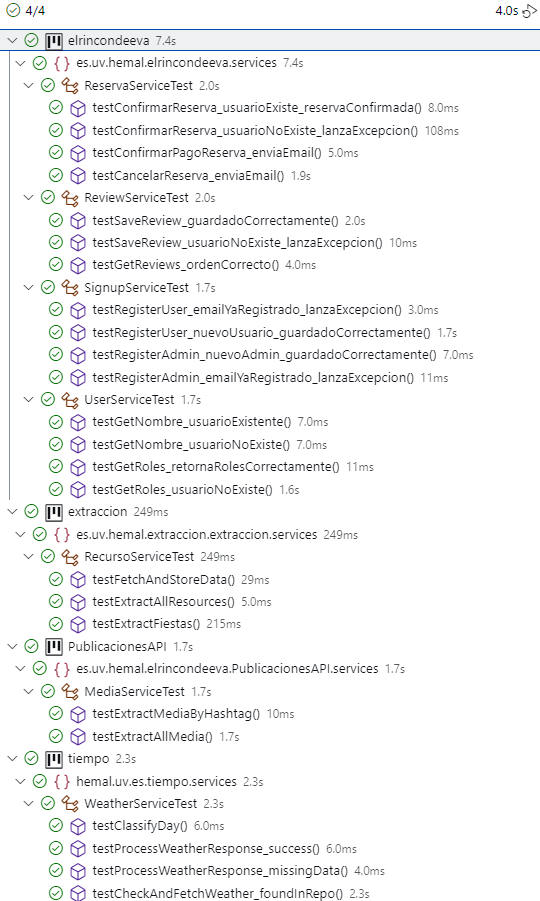
\includegraphics[width=0.5\textwidth]{figs/pruebas-unitarias.png}
\caption{Ejecución de las pruebas unitarias realizadas en el \gls{backend} de la aplicación}
\label{fig:pruebas-unitarias}
\end{figure}
    \subsection{Pruebas funcionales de la aplicación web}
Las pruebas funcionales de la aplicación web se han realizado utilizando la herramienta Cypress~\cite{cypress:web}, que permite realizar pruebas \gls{e2e} en aplicaciones web. Estas pruebas se han diseñado para verificar el correcto funcionamiento de las funcionalidades más relevantes de la aplicación, asegurando que los usuarios puedan interactuar con ella de manera efectiva y sin errores.
Las pruebas se han estructurado en diferentes archivos, cada uno de los cuales se centra en un aspecto específico de la aplicación. A continuación, se describen las pruebas más relevantes realizadas con Cypress:

\begin{itemize}
    \item \textbf{Pruebas de inicio de sesión y registro}: Se han creado pruebas para verificar que los usuarios pueden iniciar sesión correctamente con credenciales válidas y que el sistema maneja adecuadamente los errores de inicio de sesión. También se han probado los flujos de registro, asegurando que los nuevos usuarios pueden registrarse sin problemas. En el Apéndice~\ref{ap:test}, Listado~\ref{lst:loginTest} y Listado~\ref{lst:registerTest} se pueden consultar los códigos fuente de las pruebas funcionales realizadas en el inicio de sesión y registro. En estas pruebas se ha validado lo siguiente:
      \begin{itemize}
        \item \textbf{Debería iniciar sesión con credenciales válidas}: Verifica que, al ingresar un correo y una contraseña válidos, el usuario es redirigido a la página de inicio (\texttt{/inicio}).
        \item \textbf{Debería mostrar error si los datos son inválidos}: Verifica que, si se ingresan credenciales inválidas, el sistema muestra un mensaje de error indicando que el usuario o la contraseña no existen.
      \end{itemize}
      El resultado de estas pruebas para el \texttt{Login} y el \texttt{Registro} se muestran en la Figura~\ref{fig:pruebas-login} y la Figura~\ref{fig:pruebas-reserva} respectivamente.
\begin{figure}[h!tb]
\centering
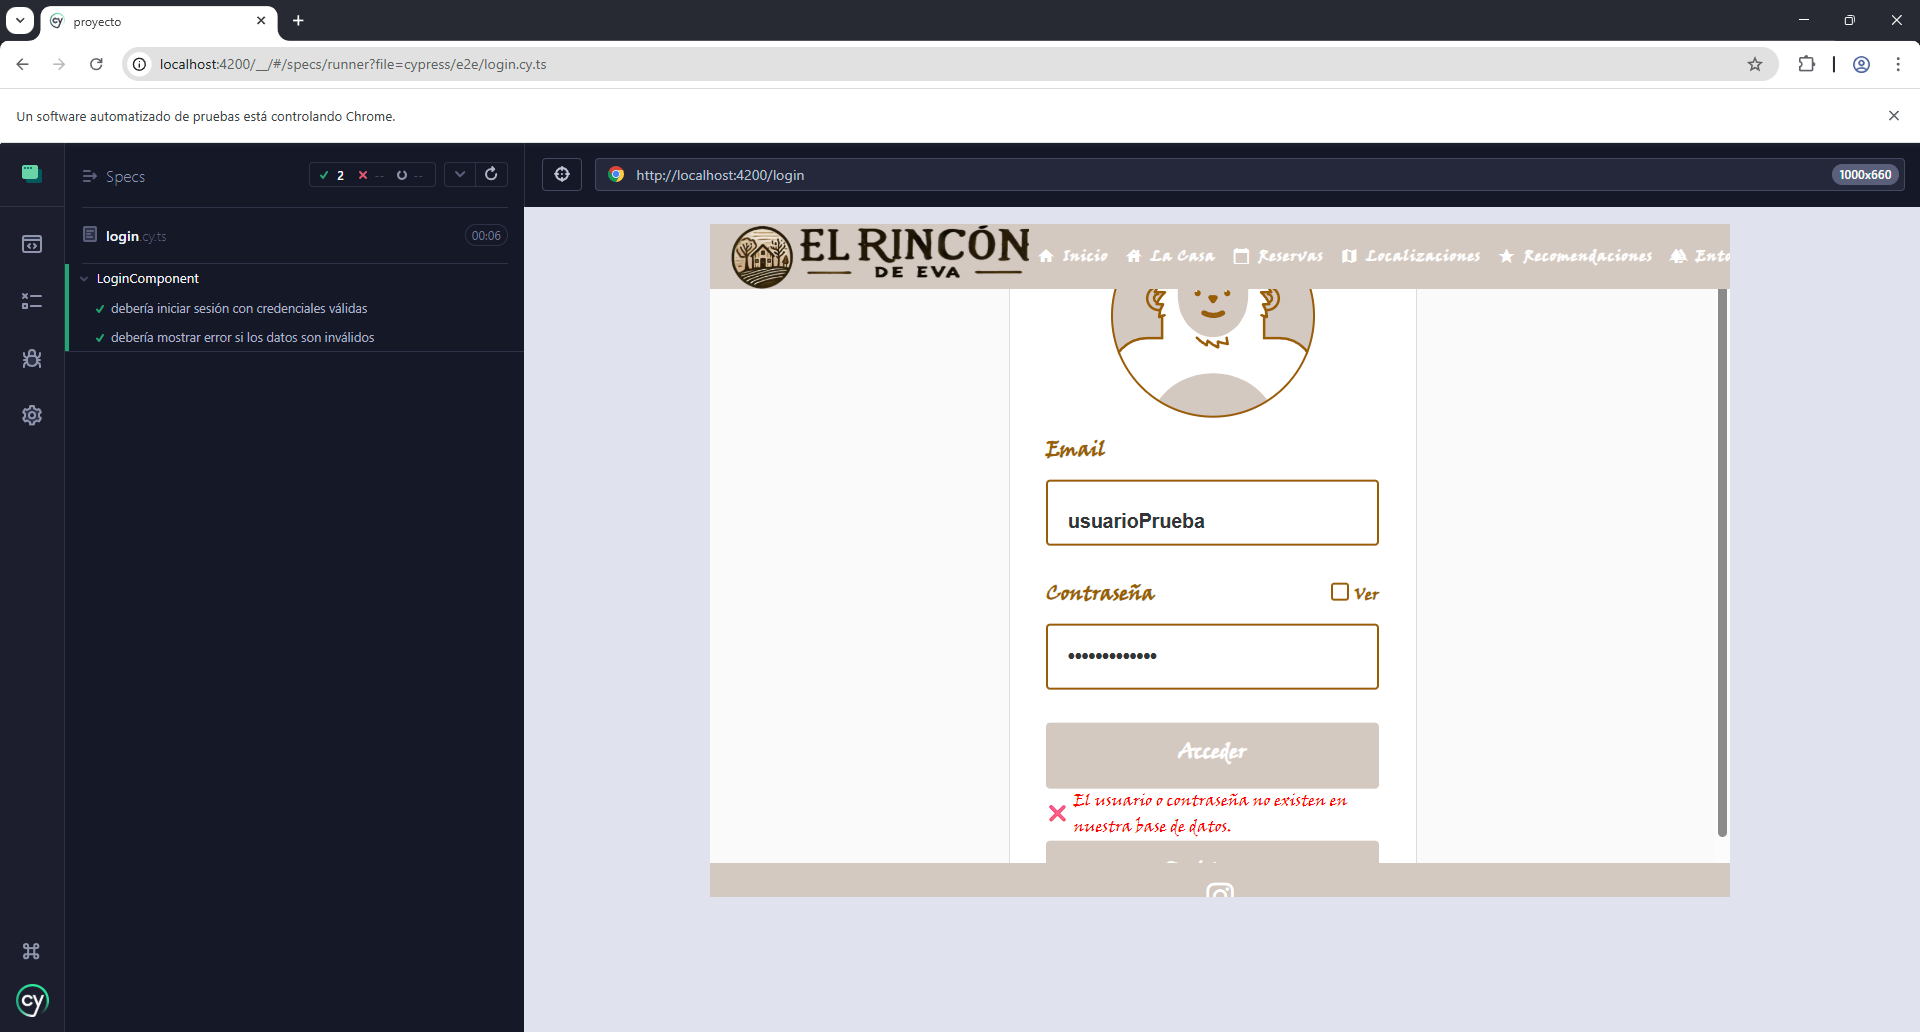
\includegraphics[width=1\textwidth]{figs/pruebasLogin.png}
\caption{Ejecución de las pruebas de inicio de sesión}
\label{fig:pruebas-login}
\end{figure}

\begin{figure}[h!tb]
\centering
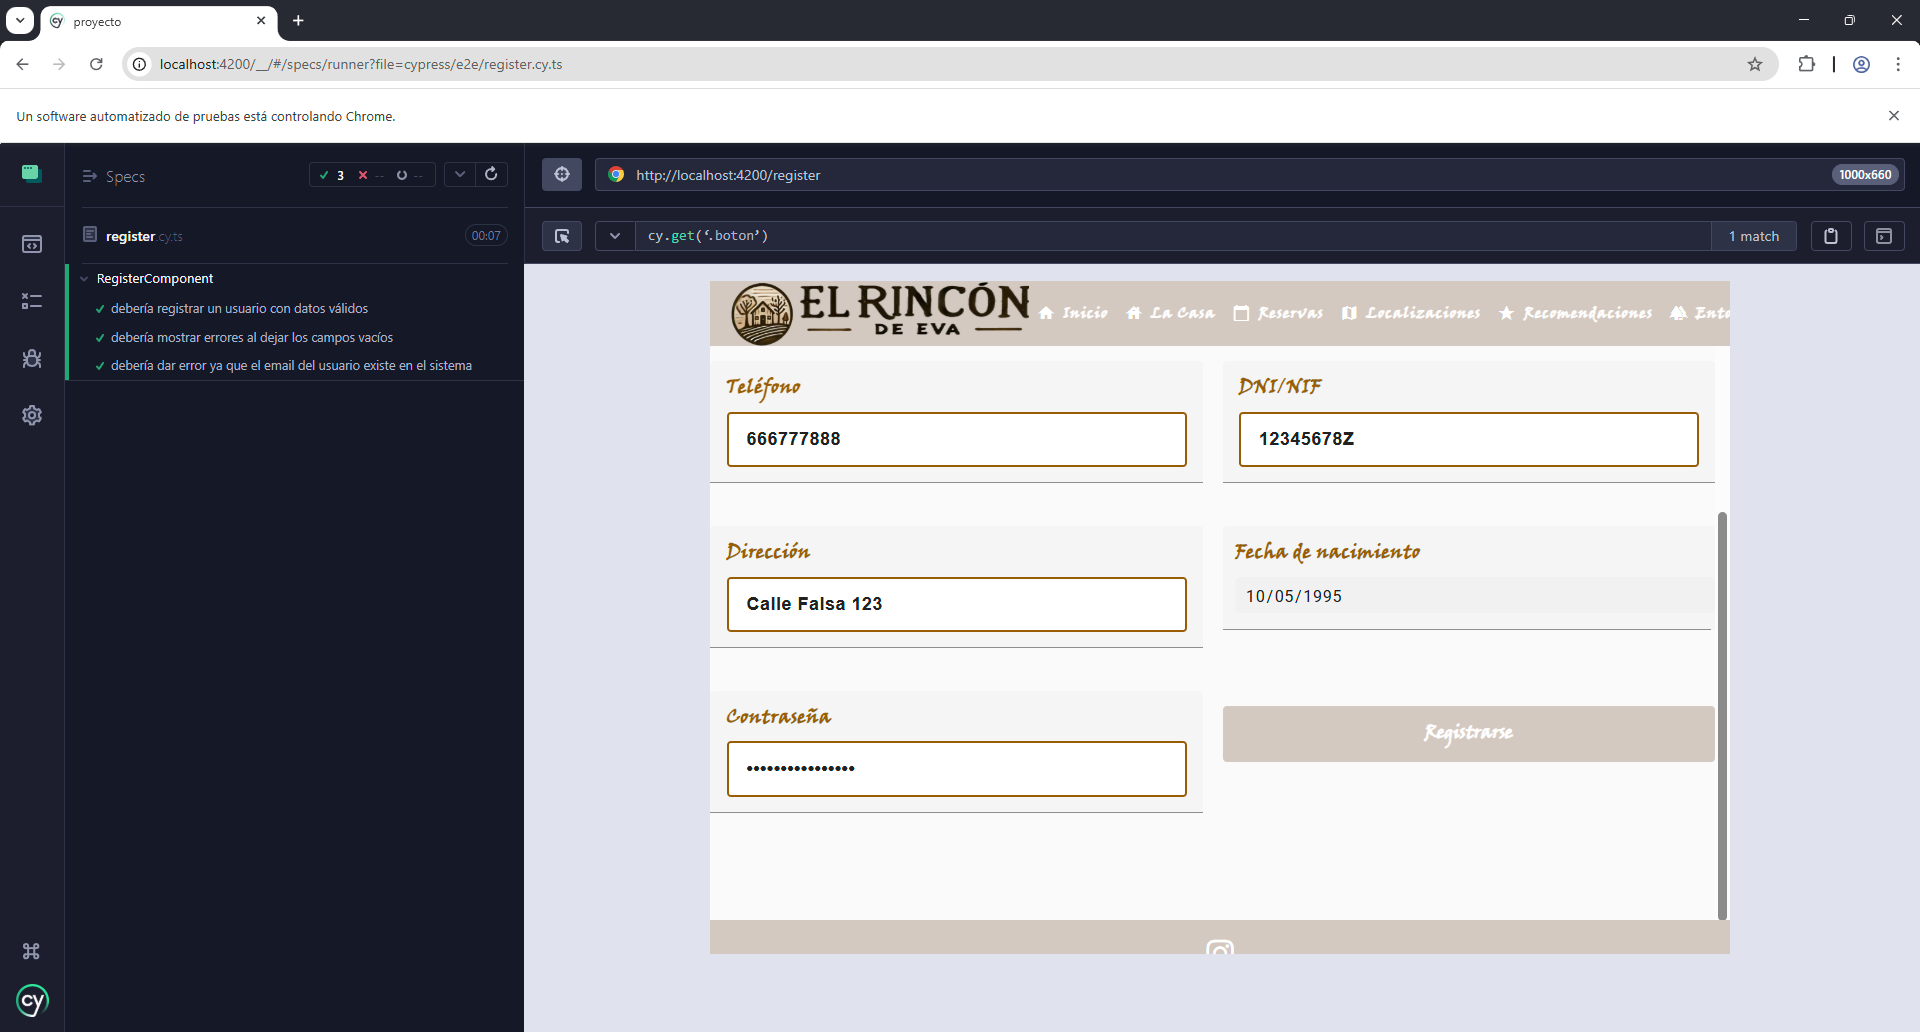
\includegraphics[width=1\textwidth]{figs/pruebasRegistro.png}
\caption{Ejecución de las pruebas de registro}
\label{fig:pruebas-registro}
\end{figure}

      \item \textbf{Pruebas de reservas}: Se han diseñado pruebas para verificar que los usuarios pueden realizar reservas correctamente, incluyendo la selección de fechas, la introducción de datos personales y la confirmación de la reserva. También se han probado los flujos de cancelación y modificación de reservas. En el Apéndice~\ref{ap:test}, Listado~\ref{lst:reservaTest} se puede consultar el código fuente de las pruebas funcionales realizadas en la gestión de reservas. En estas pruebas se ha validado lo siguiente:
      \begin{itemize}
        \item \textbf{Debe mostrar un botón para iniciar sesión cuando el email está vacío}: Verifica que se muestre un botón de inicio de sesión cuando el campo de email está vacío.
        \item \textbf{Debe mostrar el calendario de reservas cuando el email está presente}: Verifica que se muestra el calendario de reservas al iniciar sesión correctamente.
        \item \textbf{Debe mostrar el tiempo para las fechas seleccionadas}: Verifica que se muestre el tiempo para las fechas seleccionadas en el calendario.
        \item \textbf{Debe mostrar el formulario para completar la reserva rellenado desde el backend}: Verifica que el formulario de reserva esté correctamente rellenado con datos provenientes del backend.
      \end{itemize}
      El resultado de estas pruebas se muestra en la Figura~\ref{fig:pruebas-reserva}.
\begin{figure}[h!tb]
\centering
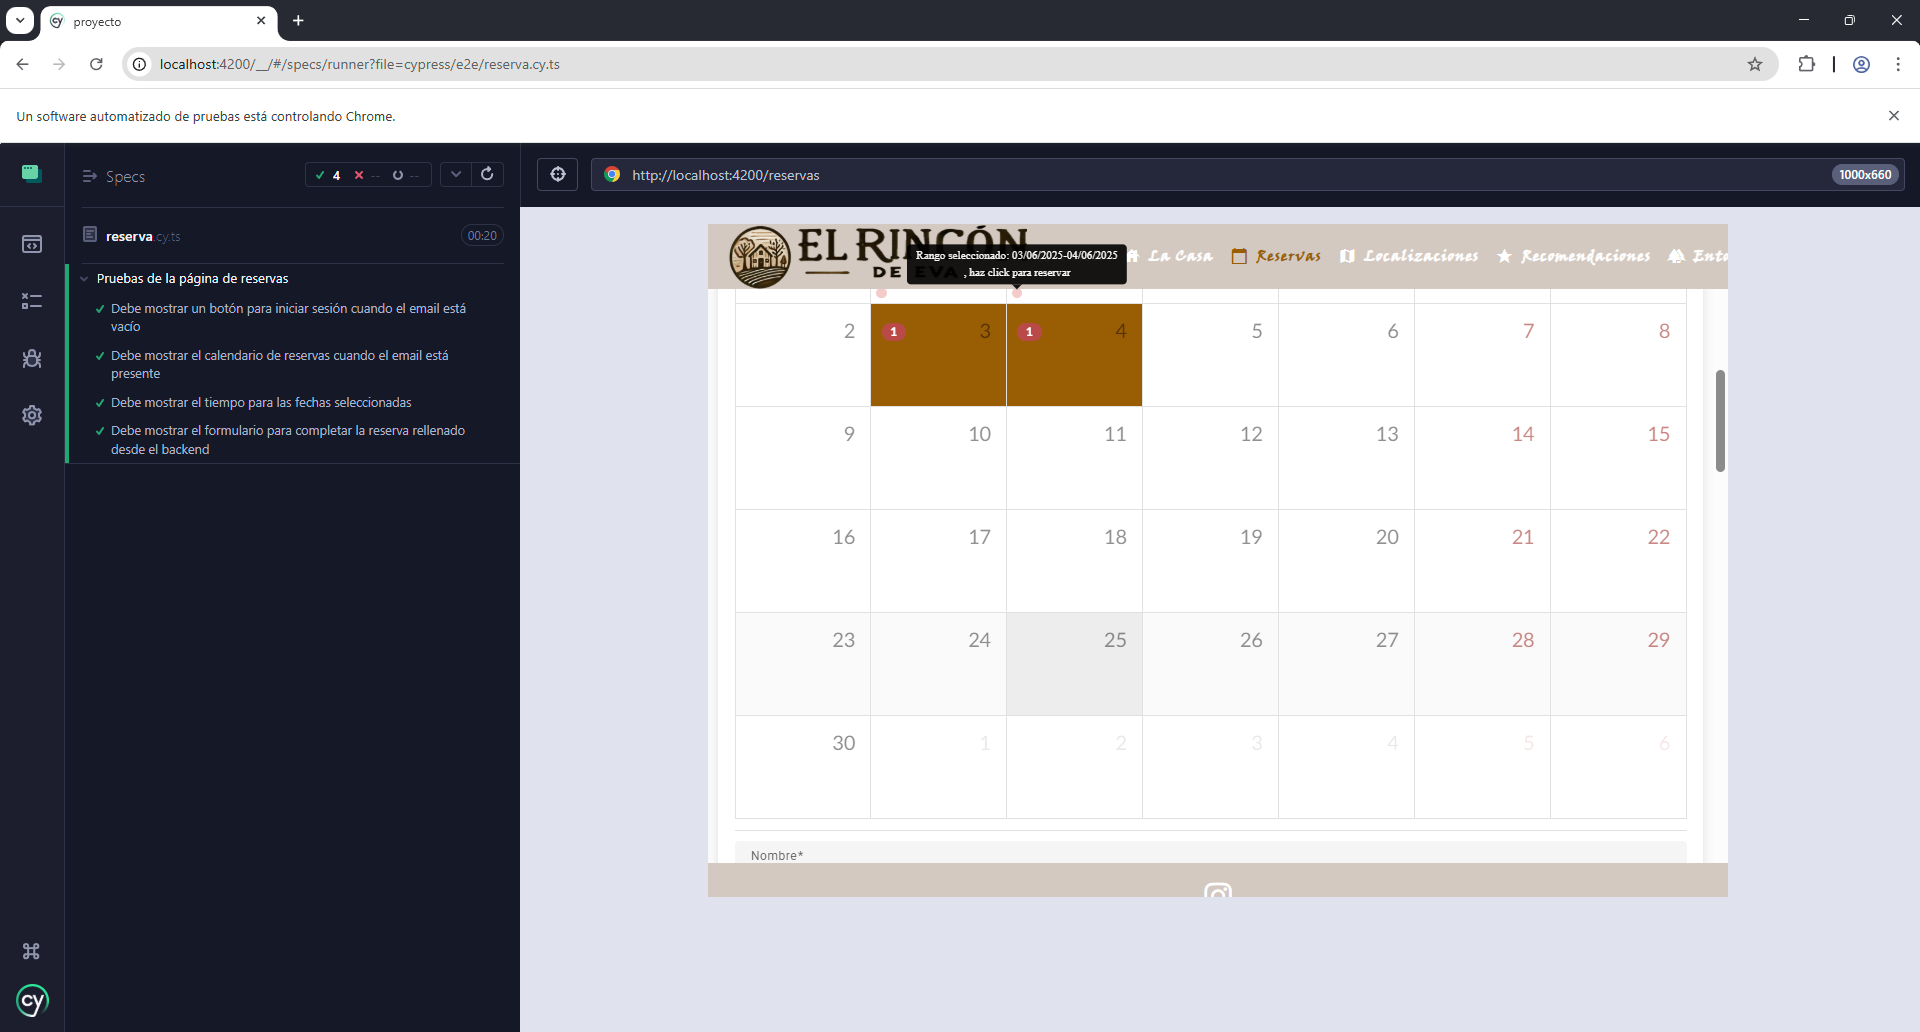
\includegraphics[width=1\textwidth]{figs/pruebasReservaTiempo.png}
\caption{Ejecución de las pruebas de reservas}
\label{fig:pruebas-reserva}
\end{figure}

    \item \textbf{Pruebas de gestión de reservas}: Se han diseñado pruebas para verificar que el administrador puede realizar gestiones sobre las reservas probando los flujos de cancelación, aprobación de reservas. En el Apéndice~\ref{ap:test}, Listado~\ref{lst:gestionTest} se puede consultar el código fuente de las pruebas funcionales realizadas en la gestión de reservas. En estas pruebas se ha validado lo siguiente:
      \begin{itemize}
  \item \textbf{Debería mostrar la tabla de reservas con encabezados correctos}: Verifica que la tabla de reservas es visible y que los encabezados incluyen: \texttt{'Nombre', 'Nº Personas', 'Estado', 'Fechas', 'Acciones'}.
  \item \textbf{Debería tener al menos una fila de datos}: Asegura que la tabla contiene al menos una fila con datos.
  \item \textbf{Debería mostrar los botones adecuados según el estado de la reserva}: Verifica que los botones de la tabla cambian dependiendo del estado de la reserva:
    \begin{itemize}
      \item Si el estado es \texttt{PAGADA} o \texttt{FINALIZADA}, el botón debería mostrar el icono \texttt{check\_circle}.
      \item Si el estado es \texttt{CANCELADA}, el botón debería mostrar el icono \texttt{error}.
      \item En otros estados, debería haber botones con iconos \texttt{check} y \texttt{close}.
    \end{itemize}
  \item \textbf{Debería aprobar una reserva CONFIRMADA, rellenar el motivo y confirmar}: 
    \begin{itemize}
      \item Hace clic en el botón de una reserva con estado \texttt{CONFIRMADA}.
      \item Espera a que se abra el diálogo, escribe el motivo en el \texttt{textarea} y hace clic en \texttt{Aceptar}.
      \item Verifica que se muestre un mensaje de éxito: \texttt{Reserva confirmada con éxito!}.
    \end{itemize}
\end{itemize}

      El resultado de estas pruebas se muestra en la Figura~\ref{fig:pruebas-gestion}.
        \begin{figure}[h!tb]
        \centering
        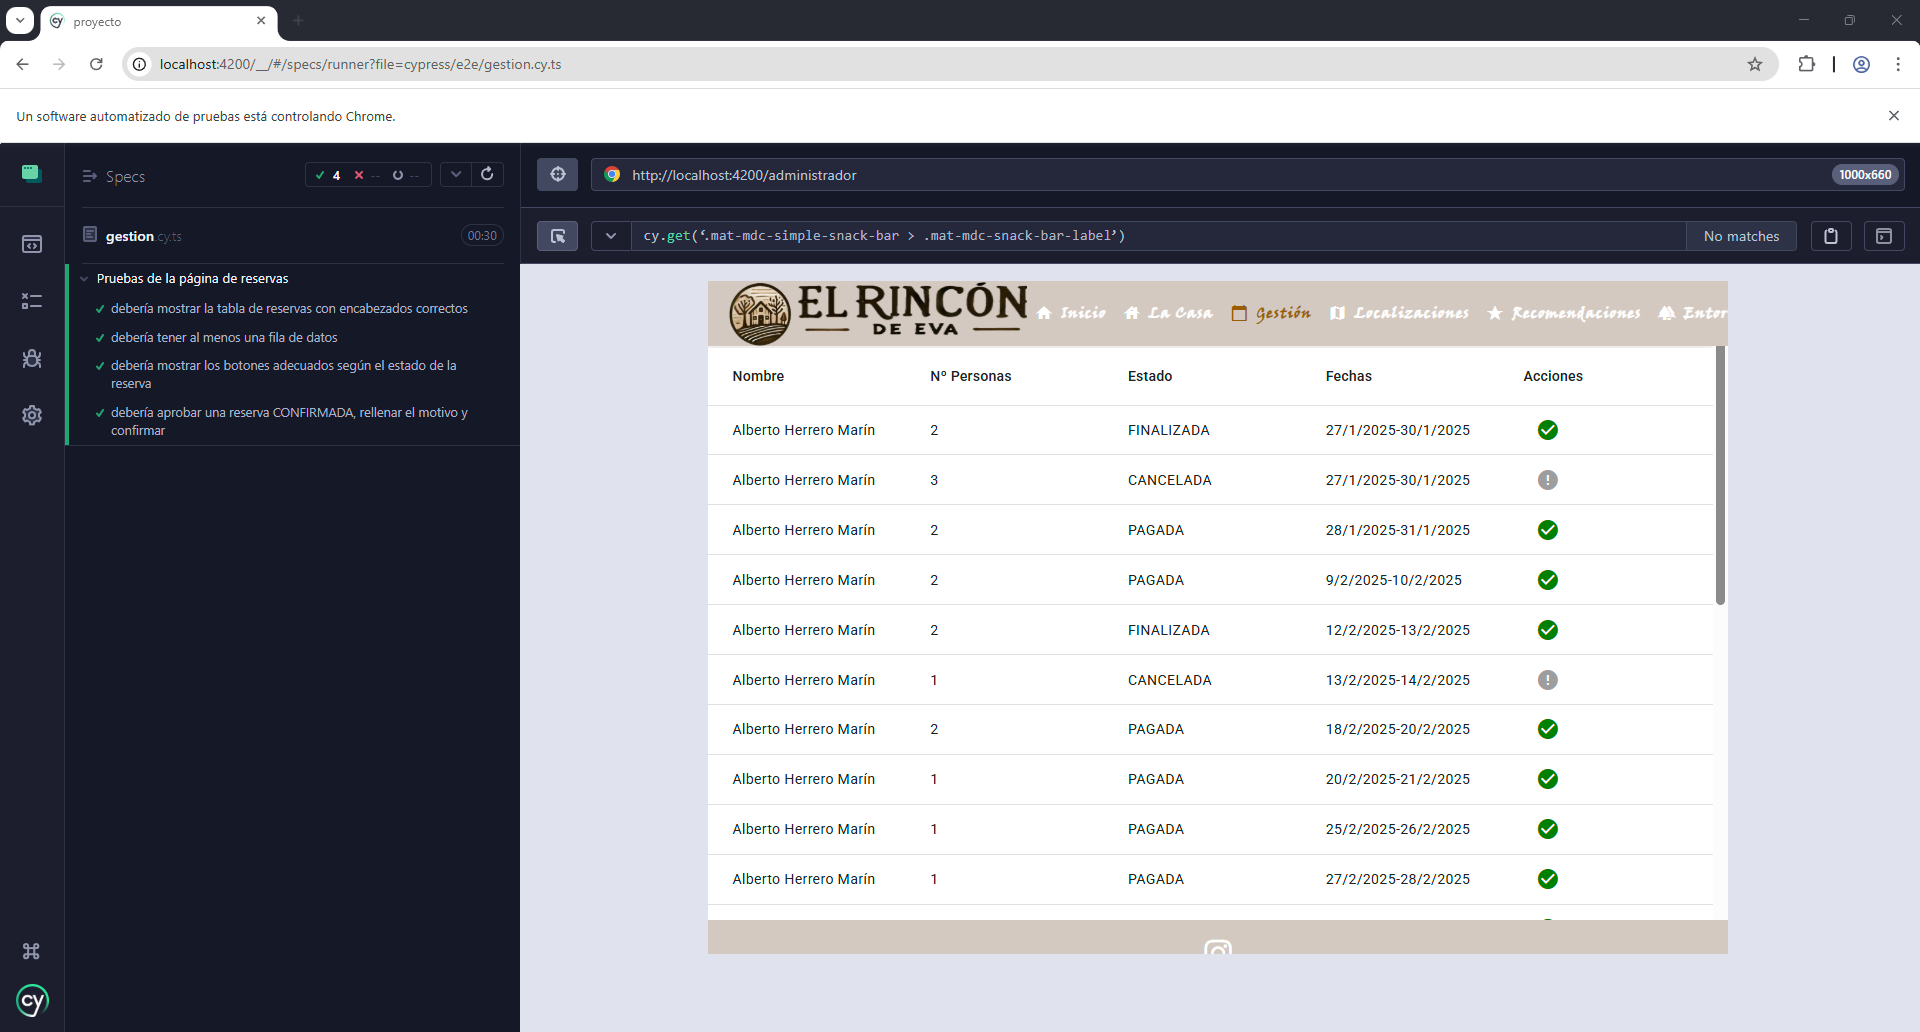
\includegraphics[width=1\textwidth]{figs/pruebasGestion.png}
        \caption{Ejecución de las pruebas de gestión de reservas}
        \label{fig:pruebas-gestion}
        \end{figure}
    \end{itemize}
Con estas pruebas y las realizadas durante las pruebas unitarias se han validado cada uno de los casos de uso definidos durante la sección de Análisis~\ref{sec:casosuso}. En la Tabla~\ref{tbl:pruebasCU} se muestran los casos de uso y las pruebas realizadas para cada uno de ellos.
	
\begin{longtable}{|p{2.5cm}|p{3.5cm}|p{4.5cm}|p{5cm}|}
\caption{Pruebas de casos de uso}
\label{tbl:pruebasCU} \\
\hline
\textbf{Caso de uso} & \textbf{Prerrequisitos} & \textbf{Prueba} & \textbf{Resultado esperado} \\
\hline
\endfirsthead

\hline
\textbf{Caso de uso} & \textbf{Prerrequisitos} & \textbf{Prueba} & \textbf{Resultado esperado} \\
\hline
\endhead

\hline
\multicolumn{4}{r}{\textit{Continúa en la siguiente página}} \\
\endfoot

\hline
\endlastfoot
		CU-1 - Login & 
		El cliente debe existir en el sistema. &
		Rellenar formulario de login y enviarlo. Validación en cliente y servidor. &
		El usuario queda autenticado y puede acceder a la sección de reservas al completo para poder realizar una nueva reserva. \\ \hline
CU-2 Logout &
Debe de existir el cliente en el sistema. \newline El cliente debe estar logueado. &
Cerrar sesión como cliente y verificar que el estado de sesión se elimina. &
El usuario volverá a ser anónimo. \newline Se eliminará cualquier estado de sesión almacenada. \newline Se limitará la posibilidad de realizar una reserva. \\ \hline

CU-3 Registrarse &
No debe de existir el email del cliente en el sistema. &
Rellenar el formulario de registro con datos válidos y enviarlo. &
El usuario estará registrado en el sistema. \newline Se añadirá un nuevo estado de sesión almacenada. \newline Se redirigirá al usuario al menú principal. \\ \hline

CU-4 Obtener información de la casa &
El servidor web se encuentre en funcionamiento. &
Acceder a la pestaña ``La casa'' y verificar que se muestran los datos y contenido multimedia. &
El usuario visualizará los datos y el contenido multimedia relacionado con la casa rural. \\ \hline

CU-5 Contactar con gestor &
El servidor web se encuentre en funcionamiento. &
Rellenar el formulario de contacto con datos válidos y enviarlo. &
En el correo del administrador se debe visualizar un nuevo correo. \\ \hline

CU-6 Obtener localización &
El servidor web se encuentre en funcionamiento. &
Acceder a la pestaña ``Dónde estamos'' y verificar que se muestra un mapa interactivo. &
Se debe visualizar un mapa interactivo situado sobre el inmueble. \\ \hline

CU-7 Obtener fiestas y gastronomía &
El servidor web se encuentre en funcionamiento. &
Acceder a la pestaña ``Recomendaciones'' y verificar que se muestra contenido textual y multimedia. &
Se debe visualizar contenido tanto estático como extraído de las redes sociales. \\ \hline

CU-8 Obtener recomendaciones turísticas &
El servidor web se encuentre en funcionamiento. &
Acceder a la pestaña ``Entorno'' y verificar que se muestra contenido multimedia con descripciones. &
Se debe visualizar contenido tanto estático como extraído de las redes sociales. \newline Si se hace clic sobre alguna, se debe redirigir al sistema origen. \\ \hline

CU-9 Obtener reseñas &
El servidor web se encuentre en funcionamiento. \newline Debe haber al menos una reseña almacenada en el servidor. &
Acceder a la pestaña ``Inicio'' y verificar que se muestra una lista de reseñas. &
Se debe visualizar una lista de reseñas que incluirán una puntuación final sobre la estancia. \\ \hline

CU-10 Obtener actividades &
El servidor web se encuentre en funcionamiento. \newline La API que proporciona las actividades debe estar en funcionamiento. &
Acceder a la pestaña ``Entorno'' y verificar que se muestran actividades con descripción y dificultad. &
Se debe visualizar un conjunto de actividades con descripción y dificultad. \newline Si se hace clic sobre alguna, se debe redirigir al sistema origen. \\ \hline

CU-11 Obtener fechas disponibles &
El servidor web se encuentre en funcionamiento. \newline Solo se mostrarán fechas a futuro. \newline Las fechas no disponibles se marcarán con un color diferente. &
Acceder a la pestaña ``Reservas'' y verificar que se muestra un calendario interactivo con las fechas disponibles. &
Se debe visualizar un calendario interactivo con las fechas disponibles y las ocupadas. \\ \hline

CU-12 Reservar fechas &
Se deben cumplir las condiciones y el flujo del CU11. \newline El servidor web se encuentre en funcionamiento. \newline Solo se podrán seleccionar fechas a futuro. \newline Las fechas no disponibles no se podrán seleccionar. \newline Deberá existir una base de datos que almacene las reservas. &
Seleccionar un conjunto de fechas disponibles, formalizar la reserva y verificar que se registra correctamente. &
Se debe visualizar un mensaje de éxito de creación de la reserva. \newline Se debe mostrar como reserva pendiente de confirmación en el perfil del cliente. \\ \hline

CU-13 Obtener clima &
Se deben cumplir las condiciones y el flujo del CU11. \newline El servidor web se encuentre en funcionamiento. \newline El servicio externo de tiempo debe estar disponible. &
Seleccionar un conjunto de fechas y verificar que se muestra el pronóstico del tiempo. &
Se debe visualizar una sección con el pronóstico de tiempo para cada uno de los días seleccionados. \\ \hline

CU-14 Obtener tarifas &
El servidor web se encuentre en funcionamiento. &
Seleccionar fechas en la pestaña ``Reservas'' y verificar que se muestran las tarifas asociadas. &
Se debe visualizar las tarifas asociadas a las fechas seleccionadas. \\ \hline

CU-15 Dejar reseña &
El servidor web se encuentre en funcionamiento. \newline El cliente registrado debe tener asignado el rol de cliente. &
Rellenar el formulario de nueva reseña con datos válidos y enviarlo. &
Se debe visualizar un mensaje de confirmación de la reseña. \newline La nueva reseña debe aparecer en la lista de reseñas. \\ \hline

CU-16 Consultar reservas pendientes &
El servidor web se encuentre en funcionamiento. \newline Debe haber al menos una reserva pendiente en el sistema. Debe estar logueado como administrador. &
Acceder a la pestaña ``Gestión'' y verificar que se muestra una lista de reservas. &
Se debe visualizar una lista de reservas pendientes de confirmación. \\ \hline

CU-17 Confirmar reserva &
El servidor web se encuentre en funcionamiento. \newline Debe haber al menos una reserva pendiente en el sistema. Debe estar logueado como administrador. &
Seleccionar una reserva pendiente y aprobarla. &
La reserva seleccionada cambiará su estado a aprobada. \newline El cliente recibirá una notificación de aprobación. \\ \hline

CU-18 Denegar reserva &
El servidor web se encuentre en funcionamiento. \newline Debe haber al menos una reserva pendiente en el sistema. Debe estar logueado como administrador. &
Seleccionar una reserva pendiente y rechazarla. &
La reserva seleccionada cambiará su estado a rechazada. \newline El cliente recibirá una notificación de rechazo. \\ \hline

CU-19 Raspar datos web &
Las aplicaciones web de los ayuntamientos deben estar disponibles. &
Ejecutar el proceso de extracción de datos y verificar que se almacenan correctamente. &
Los datos extraídos se almacenarán y se mostrarán en la aplicación web. \\ \hline

CU-20 Extraer datos actividades &
Las APIs de actividades al aire libre deben estar disponibles. &
Ejecutar el proceso de extracción de datos y verificar que se almacenan correctamente. &
Los datos extraídos se almacenarán y se mostrarán en la aplicación web. \\ \hline

CU-21 Extraer datos de redes sociales &
Las APIs de las redes sociales deben estar disponibles. &
Ejecutar el proceso de extracción de datos y verificar que se almacenan correctamente. &
Los datos extraídos se almacenarán y se mostrarán en la aplicación web. \\ \hline


	\caption{Pruebas de casos de uso}
	\label{tbl:pruebasCU}
\end{longtable}

\section{Pruebas de seguridad}
Para garantizar la seguridad de la aplicación web desarrollada, se han llevado a cabo pruebas de seguridad utilizando la herramienta OWASP ZAP~\cite{owasp-zap:web}, reconocida por su capacidad para detectar vulnerabilidades comunes en entornos web como \gls{xss}, \gls{sqlinjection}, problemas de cabeceras HTTP, entre otras. La evaluación se ha realizado sobre dos vectores principales: el \gls{backend} de la aplicación, a través de su especificación \gls{openapi} generada mediante Swagger~\cite{swagger}, y el \gls{frontend}, accediendo a la URL dónde se encuentra el servidor de Angular en funcionamiento.

\subsection{Configuración del entorno de pruebas}
La herramienta OWASP ZAP se ha ejecutado en modo GUI, atacando dos URLs principales:
\begin{itemize}
    \item \url{localhost:8089} correspondiente al frontend desplegado en un servidor embebido.
    \item \url{localhost:8080/api/v1} endpoint principal del \gls{backend}.
\end{itemize}
Para el análisis del \gls{backend}, se ha importado el archivo de especificación \gls{openapi}, \texttt{api-docs.yaml} generado automáticamente por la extensión Swagger. Esto ha permitido una exploración exhaustiva y estructurada de los endpoints.

\subsection{Pruebas de seguridad del backend}

\subsubsection{Análisis inicial}
El análisis inicial realizado con OWASP ZAP sobre el \gls{backend} identificó dos alertas relevantes, tal y como muestra la Figura~\ref{fig:alertas-zap-backend-iniciales}:

\begin{itemize}
  \item \textbf{Format String Error}: Esta alerta apareció en el endpoint \texttt{POST /api/v1/contact}. Indica que hay una posible vulnerabilidad relacionada con el tratamiento inadecuado de cadenas, potencialmente explotable para provocar errores o comportamientos no deseados si no se validan o escapan adecuadamente los datos introducidos por el usuario.
  
  \item \textbf{Inyección XSLT}: Sugiere que ciertos parámetros pueden ser susceptibles a técnicas de inyección de transformaciones XML (XSLT). Esto representa un riesgo cuando se procesan entradas \gls{xml} sin validación o filtrado.
\end{itemize}

\begin{figure}[h!tb]
    \centering
    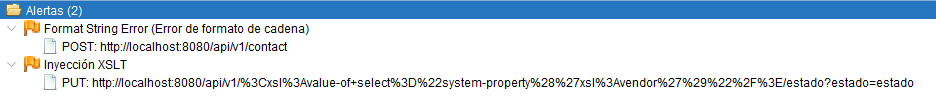
\includegraphics[width=1\textwidth]{figs/alertas_previo.png}
    \caption{Alertas iniciales detectadas en el backend por OWASP ZAP.\label{fig:alertas-zap-backend-iniciales}}
\end{figure}



\subsubsection{Medidas aplicadas}
Para solventar las vulnerabilidades detectadas se aplicaron las siguientes medidas:
\begin{itemize}
    \item Se configuraron cabeceras de seguridad en el \texttt{WebSecurityConfigurerAdapter}.
    \item Se validaron y sanearon los campos de entrada en formularios, especialmente en el \texttt{ContactService}.
\end{itemize}

\subsubsection{Resultado final}
Tras aplicar las mejoras mencionadas, se repitieron las pruebas con OWASP ZAP y ya no se observó ninguna alerta.

\subsection{Pruebas de seguridad del frontend}
\subsubsection{Análisis inicial}
Durante el análisis inicial del frontend se detectaron varias alertas de seguridad que ponían en riesgo la integridad de la aplicación web, tal y como se muestra en la Figura~\ref{fig:pruebas-seguridad-frontend}:

\begin{itemize}
    \item Falta de definición de la directiva \texttt{default-src} en la política \gls{csp}.
    \item Ausencia total o configuración incorrecta de la política \texttt{Content-Security-Policy}.
    \item Falta de cabecera \texttt{X-Frame-Options} para prevenir ataques de clickjacking.
    \item Divulgación de información mediante la cabecera HTTP \texttt{X-Powered-By}.
    \item Falta de la cabecera \texttt{X-Content-Type-Options}.
    \item Inclusión de archivos JavaScript externos de dominios cruzados.
    \item Comentarios HTML con información sensible en el código fuente.
\end{itemize}

\begin{figure}[h!tb]
    \centering
    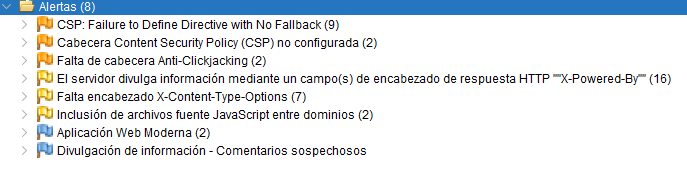
\includegraphics[width=1\textwidth]{figs/alertas_previo_front.png}
    \caption{Resultado inicial de las pruebas de seguridad del frontend.\label{fig:pruebas-seguridad-frontend}}
\end{figure}

\subsubsection{Medidas aplicadas}
\begin{itemize}
    \item Se implementó una cabecera \texttt{Content-Security-Policy} que limita las fuentes de scripts, estilos e imágenes a dominios de confianza.
    \item Se añadió la cabecera \texttt{X-Frame-Options: DENY} para evitar la incrustación de la aplicación en iframes.
    \item Se configuró la cabecera \texttt{X-Content-Type-Options: nosniff} para prevenir ataques de tipo MIME sniffing.
    \item Se eliminó la cabecera \texttt{X-Powered-By} del backend para evitar divulgación innecesaria.
    \item Se revisaron y limpiaron comentarios sospechosos o informativos en el HTML de las plantillas.
    \item Se deshabilitó la carga de archivos JS desde dominios cruzados no controlados.
\end{itemize}


\subsubsection{Resultado final}
El segundo análisis evidenció una reducción significativa de las vulnerabilidades detectadas. En la Figura~\ref{fig:pruebas-seguridad-frontend-final} se observa una situación mucho más controlada y segura. Solo quedarón dos alertas inevitables dado que Angular inyecta los estilos en formato \texttt{inline} y se ha realizado la configuración de \gls{csp} más restrictiva posible.

\begin{figure}[h!tb]
    \centering
    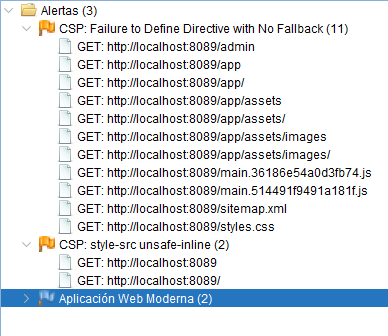
\includegraphics[width=0.6\textwidth]{figs/alertas_post_front.png}
    \caption{Resultado final de las pruebas de seguridad del frontend.\label{fig:pruebas-seguridad-frontend-final}}
\end{figure}

\section{Pruebas de rendimiento}
Para evaluar el rendimiento de la aplicación web en condiciones de carga, se ha utilizado Apache JMeter~\cite{jmeter:web}, una herramienta ampliamente reconocida para pruebas de carga y estrés. Estas pruebas permiten identificar cuellos de botella, tiempos de respuesta y comportamiento ante múltiples usuarios concurrentes.

\subsection{Configuración del entorno de pruebas}
Se ha elaborado un plan de pruebas, representado mediante un archivo \texttt{.jmx}, con el objetivo de simular múltiples usuarios concurrentes interactuando con los principales servicios expuestos por la \gls{API} \gls{rest}~\cite{kotstein2021restdelphi} del \gls{backend}. Con el fin de reproducir un entorno lo más cercano posible al de producción, dichas pruebas se han ejecutado sobre el clúster de \gls{kubernetes} previamente desplegado, al cual se accede a través de un túnel seguro establecido desde el servidor local que aloja la aplicación web del \gls{frontend}. Para estas pruebas tanto el \gls{frontend} como el cluster estarán cifrados mediante protocolo \gls{ssl}, asemejándose así a un escenario real. Los escenarios contemplados en este plan de pruebas son los siguientes:


\begin{itemize}
    \item Inicio de sesión de usuarios.
    \item Realización de reservas.
    \item Consulta de recomendaciones, actividades y entorno.
\end{itemize}

Para cada escenario se ha considerado una prueba de carga diferente. Ya que hay llamadas a \glspl{API} externas que pueden denegar el acceso si se realizan demasiadas llamadas. Además, por funcionalidad de aplicación hay pruebas de rendimiento que se realizarán siendo realistas con la finalidad de la plataforma. 

Por lo tanto, para el escenario en que se prueba un gran número de accesos concurrentes, el entorno se configuró con:
\begin{itemize}
    \item 100 usuarios virtuales concurrentes.
    \item Ramp-up de 1 segundos. Ya que no sale de la aplicación y se puede medir el rendimiento sin riesgo a que \glspl{API} externas denieguen el acceso.
    \item Duración de prueba: 5 iteraciones.
\end{itemize}
Para el escenario de generación de reservas, se configuró el entorno con:
\begin{itemize}
    \item 10 usuarios virtuales concurrentes.
    \item Ramp-up de 3 segundos. Ya que se quiere probar el caso en que varios usuarios realizan reservas al mismo tiempo, pero no se quiere saturar el sistema.
    \item Duración de prueba: 5 iteraciones.
\end{itemize}
Por último, para el escenario de consulta de recomendaciones, actividades y entorno, se configuró el entorno con:
\begin{itemize}
    \item 100 usuarios virtuales concurrentes.
    \item Ramp-up de 1 segundos. Ya que no se realizan cambios en la base de datos y se pueden realizar muchas consultas sin riesgo a que \glspl{API} externas denieguen el acceso.
    \item Duración de prueba: 5 iteraciones.
\end{itemize}
Se utilizó un \texttt{Thread Group} para cada uno de los escenarios, permitiendo así una ejecución independiente y controlada de cada prueba. Se utilizó un \texttt{HTTP(S) Test Script Recorder} para capturar las peticiones \gls{https} realizadas por el navegador al interactuar con la aplicación web. Esto permite simular de manera precisa las acciones de los usuarios reales. En la Figura~\ref{fig:jmeter-config} se muestra la configuración del entorno de pruebas en JMeter.
\begin{figure}[h!tb]
\centering
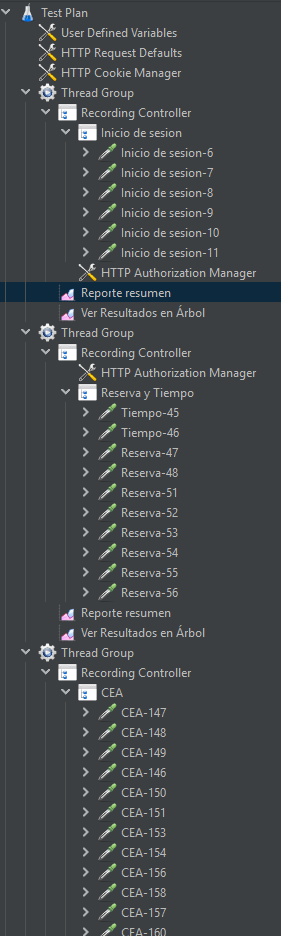
\includegraphics[width=0.4\textwidth]{figs/jmeter-config.png}
\caption{Configuración del entorno de pruebas en JMeter}
\label{fig:jmeter-config}
\end{figure}

\subsection{Resultados obtenidos}

Durante la ejecución de las pruebas de carga se ha medido la latencia media por cada endpoint, extrayendo estos datos del Reporte de Resumen generado de cada Thread Group.

La Figura~\ref{fig:latencia-inicio} representa los resultados obtenidos durante el proceso de inicio de sesión. En ella se observa un comportamiento eficiente con tiempos de respuesta bajos, lo que indica que las operaciones de autenticación están bien optimizadas y no dependen de servicios externos.

En la Figura~\ref{fig:latencia-reserva}, correspondiente al proceso de gestión de reservas, se identifican endpoints con una mayor latencia. Esta diferencia se debe principalmente a que estas operaciones requieren lógica adicional, como la comprobación de fechas disponibles o el envío de correos electrónicos, lo que implica llamadas a APIs externas.

Por último, la Figura~\ref{fig:latencia-visual} muestra la latencia media durante la carga de vistas y elementos del frontend. De nuevo, los endpoints con mayor tiempo de respuesta son aquellos que consultan servicios externos, como la obtención de datos turísticos o recomendaciones personalizadas.

\begin{figure}[h!tb]
  \centering
  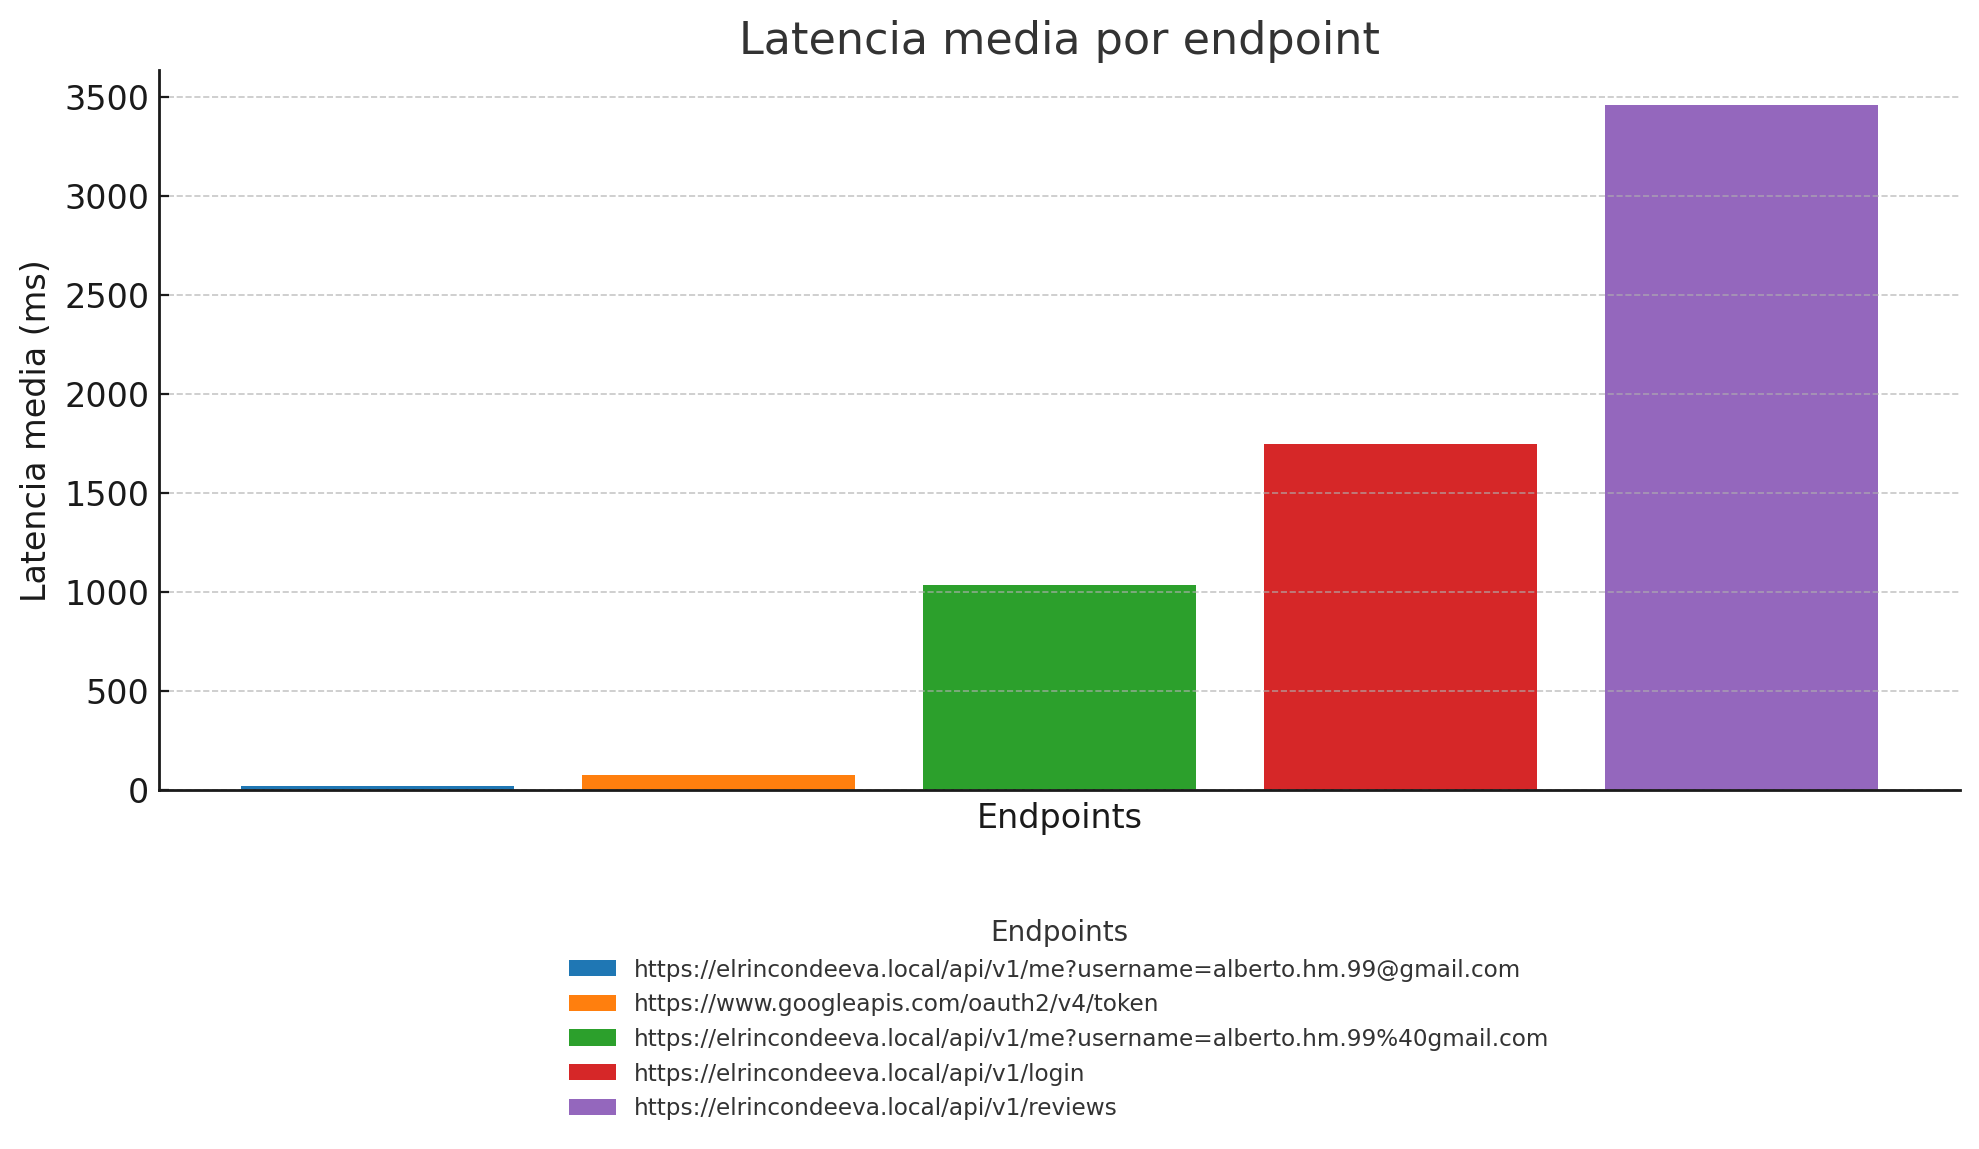
\includegraphics[width=1\textwidth]{figs/inicioyreviews.png}
  \caption{Latencia media por endpoint — datos de \texttt{inicio1.csv}}
  \label{fig:latencia-inicio}
\end{figure}

\begin{figure}[h!tb]
  \centering
  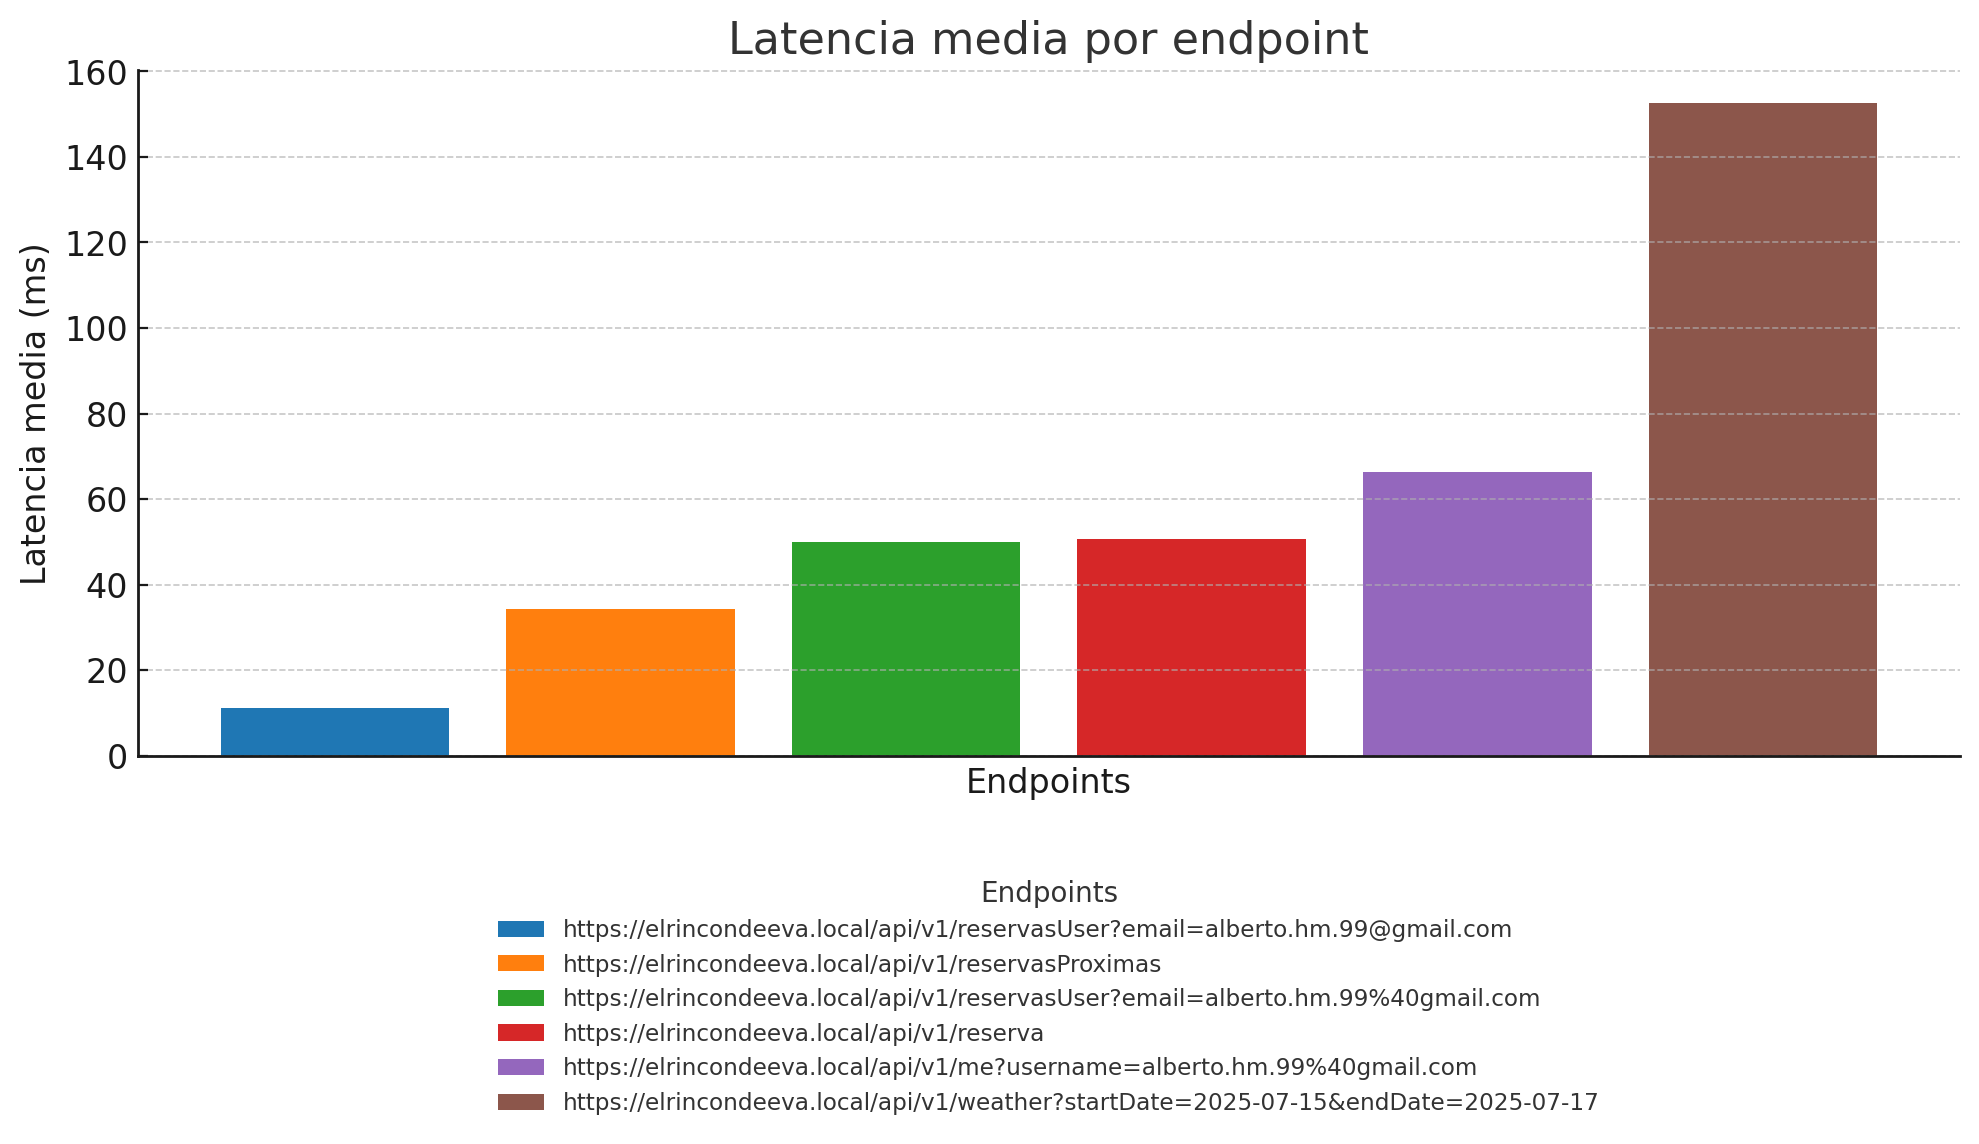
\includegraphics[width=1\textwidth]{figs/tiempoyreservas.png}
  \caption{Latencia media por endpoint — datos de \texttt{reserva1.csv}}
  \label{fig:latencia-reserva}
\end{figure}

\begin{figure}[h!tb]
  \centering
  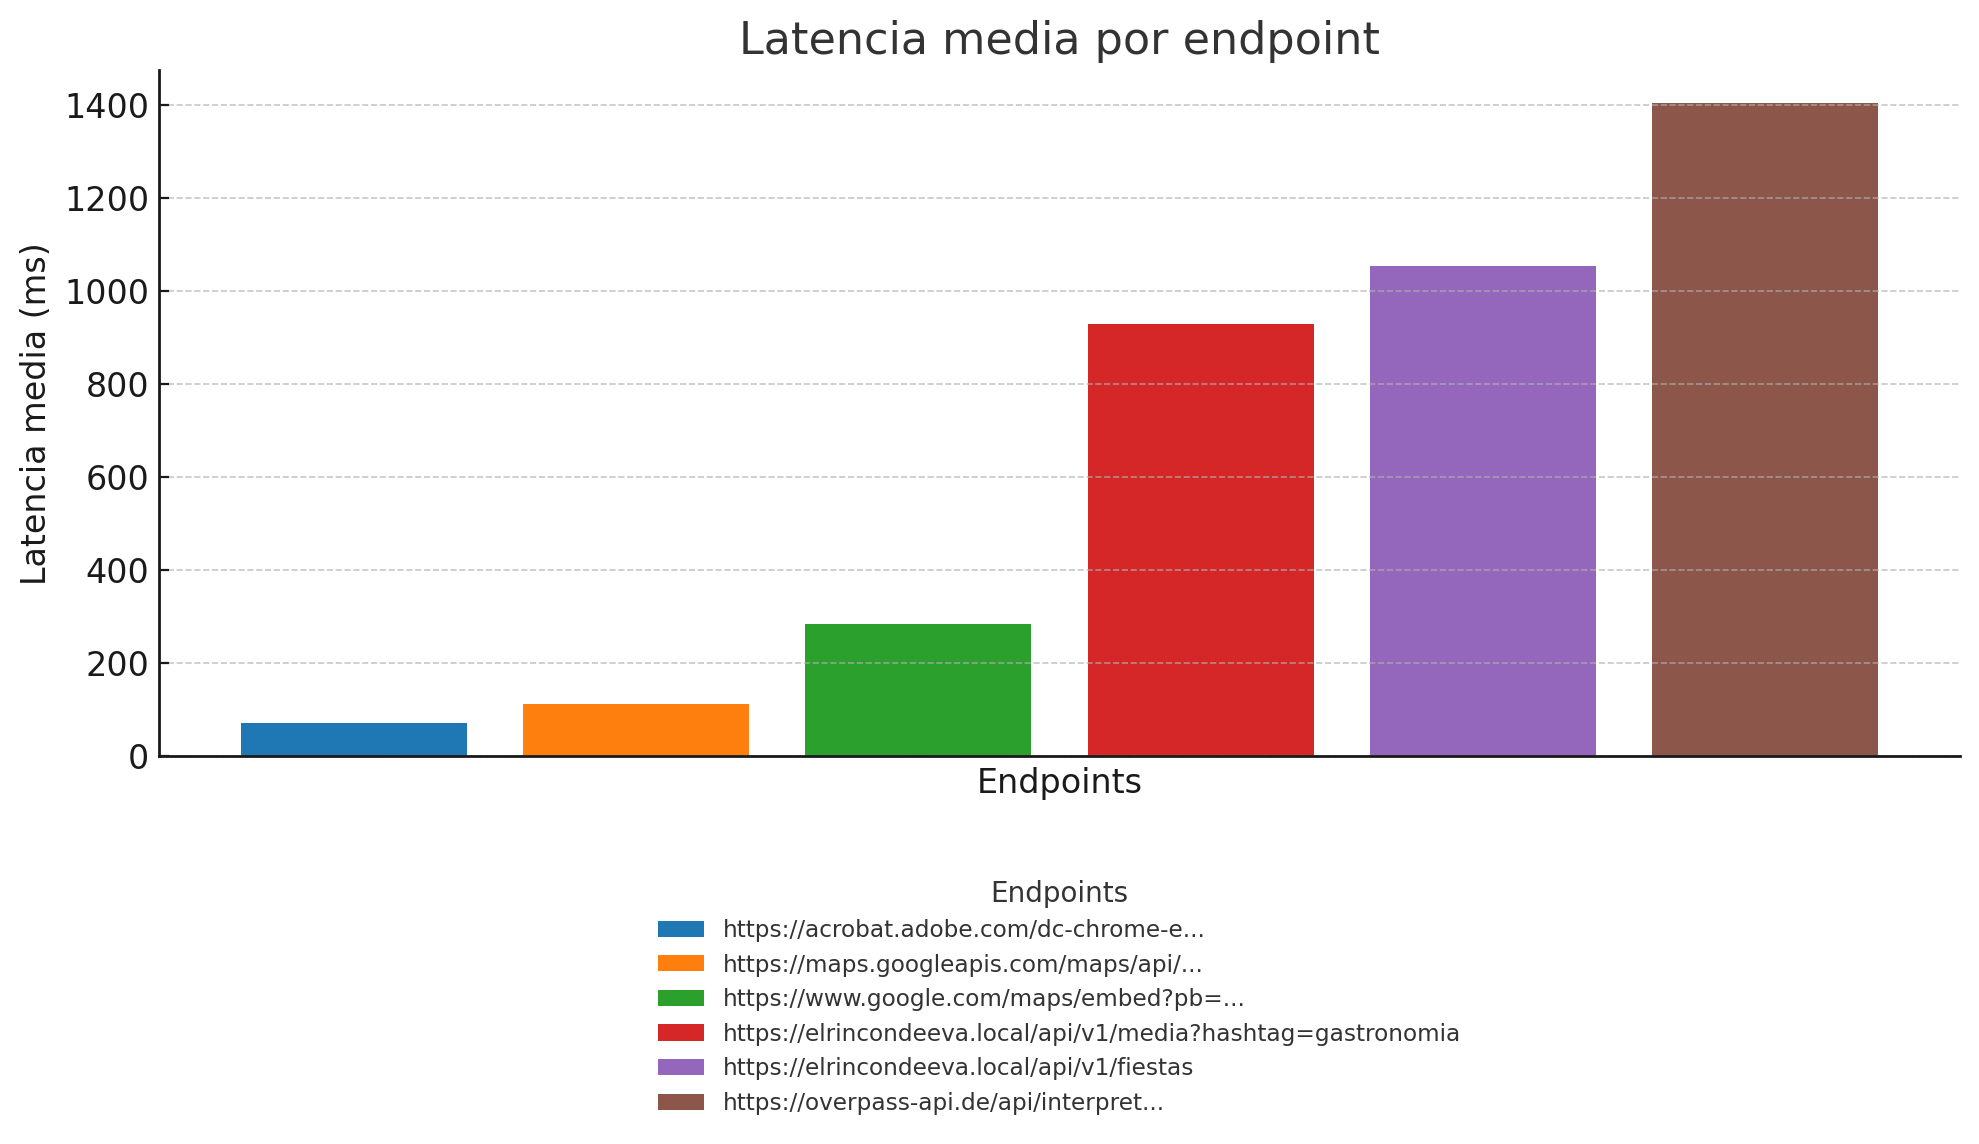
\includegraphics[width=1\textwidth]{figs/entornoyactividades.png}
  \caption{Latencia media por endpoint — datos de \texttt{visual1.csv}}
  \label{fig:latencia-visual}
\end{figure}

Los resultados obtenidos evidencian que algunos endpoints presentan una latencia significativamente mayor debido a su dependencia de servicios externos. Como trabajo futuro, se propone analizar estos casos en profundidad y aplicar mecanismos de optimización, como la implementación de caché, reducción de llamadas redundantes o estrategias de precarga, con el objetivo de mejorar el rendimiento global de la aplicación.

\clearpage
\section{Pruebas de accesibilidad y posicionamiento}

Con el fin de evaluar la calidad técnica de la aplicación web en aspectos de accesibilidad, posicionamiento, \gls{seo}, y rendimiento general, se ha ejecutado Lighthouse~\cite{lighthouse:web} sobre las principales páginas del sitio. A continuación, se resumen los resultados obtenidos, acompañados de los gráficos generados automáticamente por la herramienta.

\subsection*{Página de inicio}

\begin{figure}[h!tb]
  \centering
  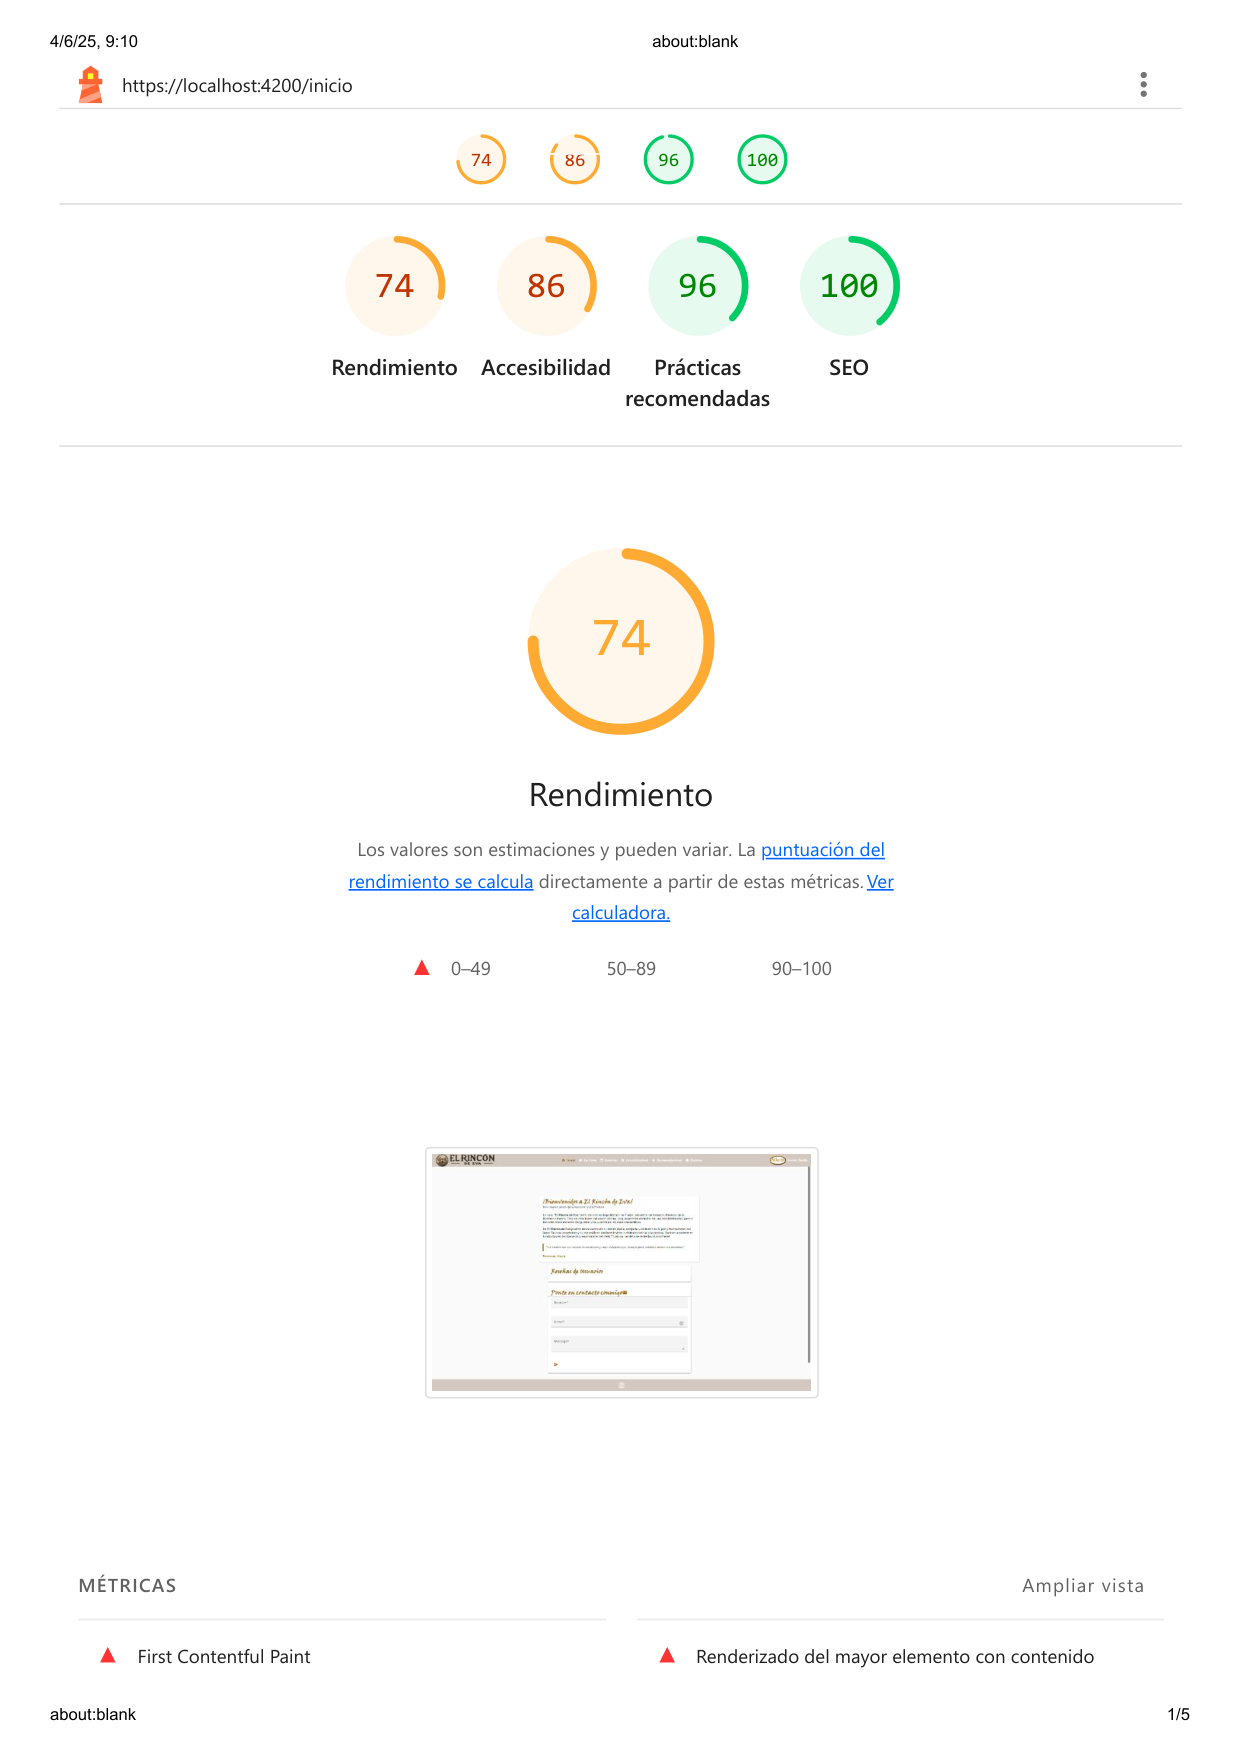
\includegraphics[width=0.85\textwidth]{figs/inicio_lighthouse.png}
  \caption{Resultados Lighthouse — Página de inicio}
  \label{fig:lighthouse-inicio}
\end{figure}

La página de inicio obtiene una puntuación destacada en \gls{seo} (100) y buenas prácticas (96), mientras que la accesibilidad se sitúa en un 86. Se detectan algunos problemas menores en botones y enlaces que carecen de etiquetas accesibles, así como contrastes de color mejorables. El rendimiento es aceptable (74), aunque se puede mejorar la carga inicial mediante compresión y reducción de JavaScript innecesario.

\subsection*{Página de entorno}

\begin{figure}[h!tb]
  \centering
  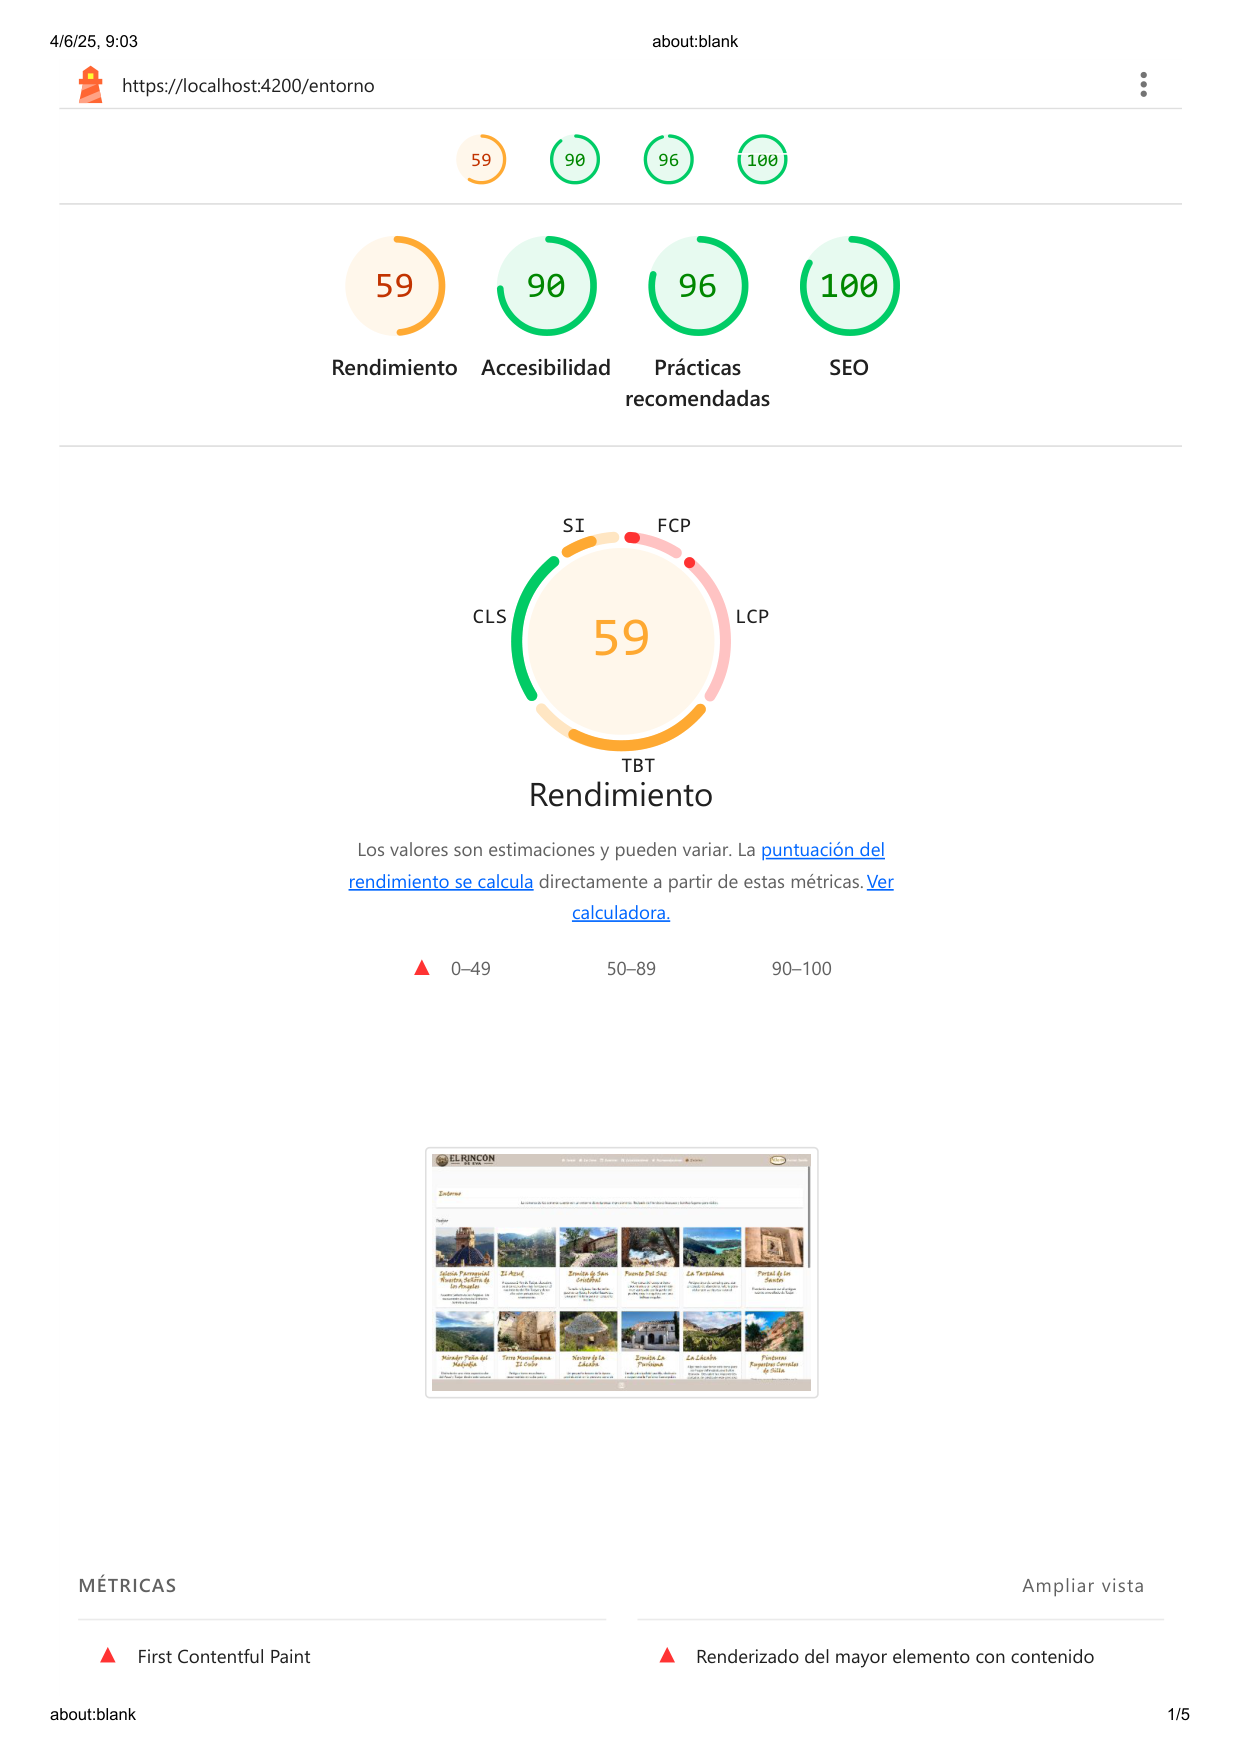
\includegraphics[width=0.85\textwidth]{figs/entorno_lighthouse.png}
  \caption{Resultados Lighthouse — Página de entorno}
  \label{fig:lighthouse-entorno}
\end{figure}

En este caso, la accesibilidad alcanza un 90 y el \gls{seo} mantiene el 100. Sin embargo, el rendimiento baja a 59, con una \gls{lcp} cercana a los 7 segundos. Se recomienda optimizar las imágenes, precargar las que son clave para el renderizado y revisar la carga de recursos bloqueantes. También se observan advertencias sobre contraste de color y etiquetas ALT redundantes.

\subsection*{Página “La casa”}

\begin{figure}[h!tb]
  \centering
  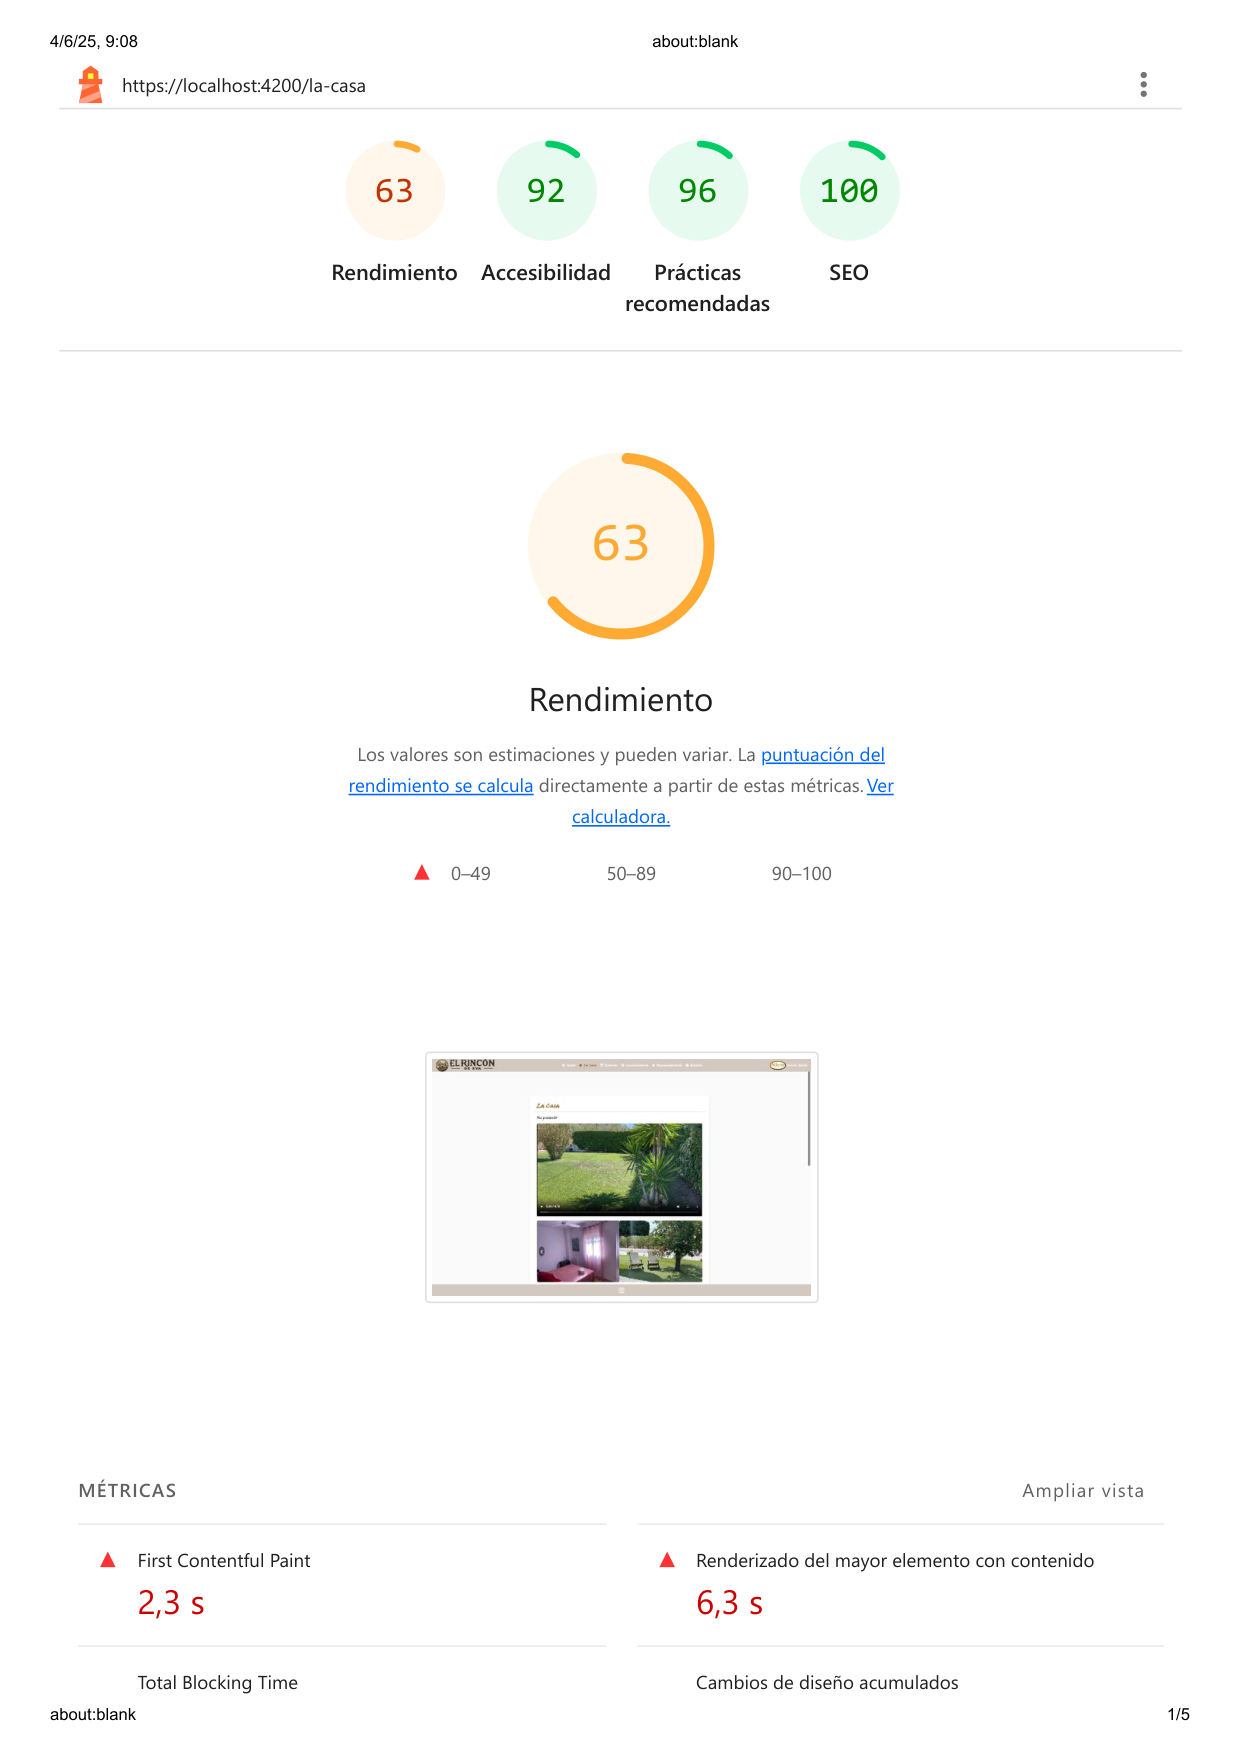
\includegraphics[width=0.85\textwidth]{figs/la_casa_lighthouse.png}
  \caption{Resultados Lighthouse — Página “La casa”}
  \label{fig:lighthouse-la-casa}
\end{figure}

El análisis muestra una accesibilidad de 92 y puntuación perfecta en \gls{seo}. El rendimiento es bajo (63), principalmente debido a la carga tardía de elementos visuales. Las recomendaciones apuntan a reducir \gls{css} y \gls{javascript} no utilizados, definir tamaños explícitos para imágenes y adoptar formatos modernos como WebP.

\subsection*{Página de localizaciones}

\begin{figure}[h!tb]
  \centering
  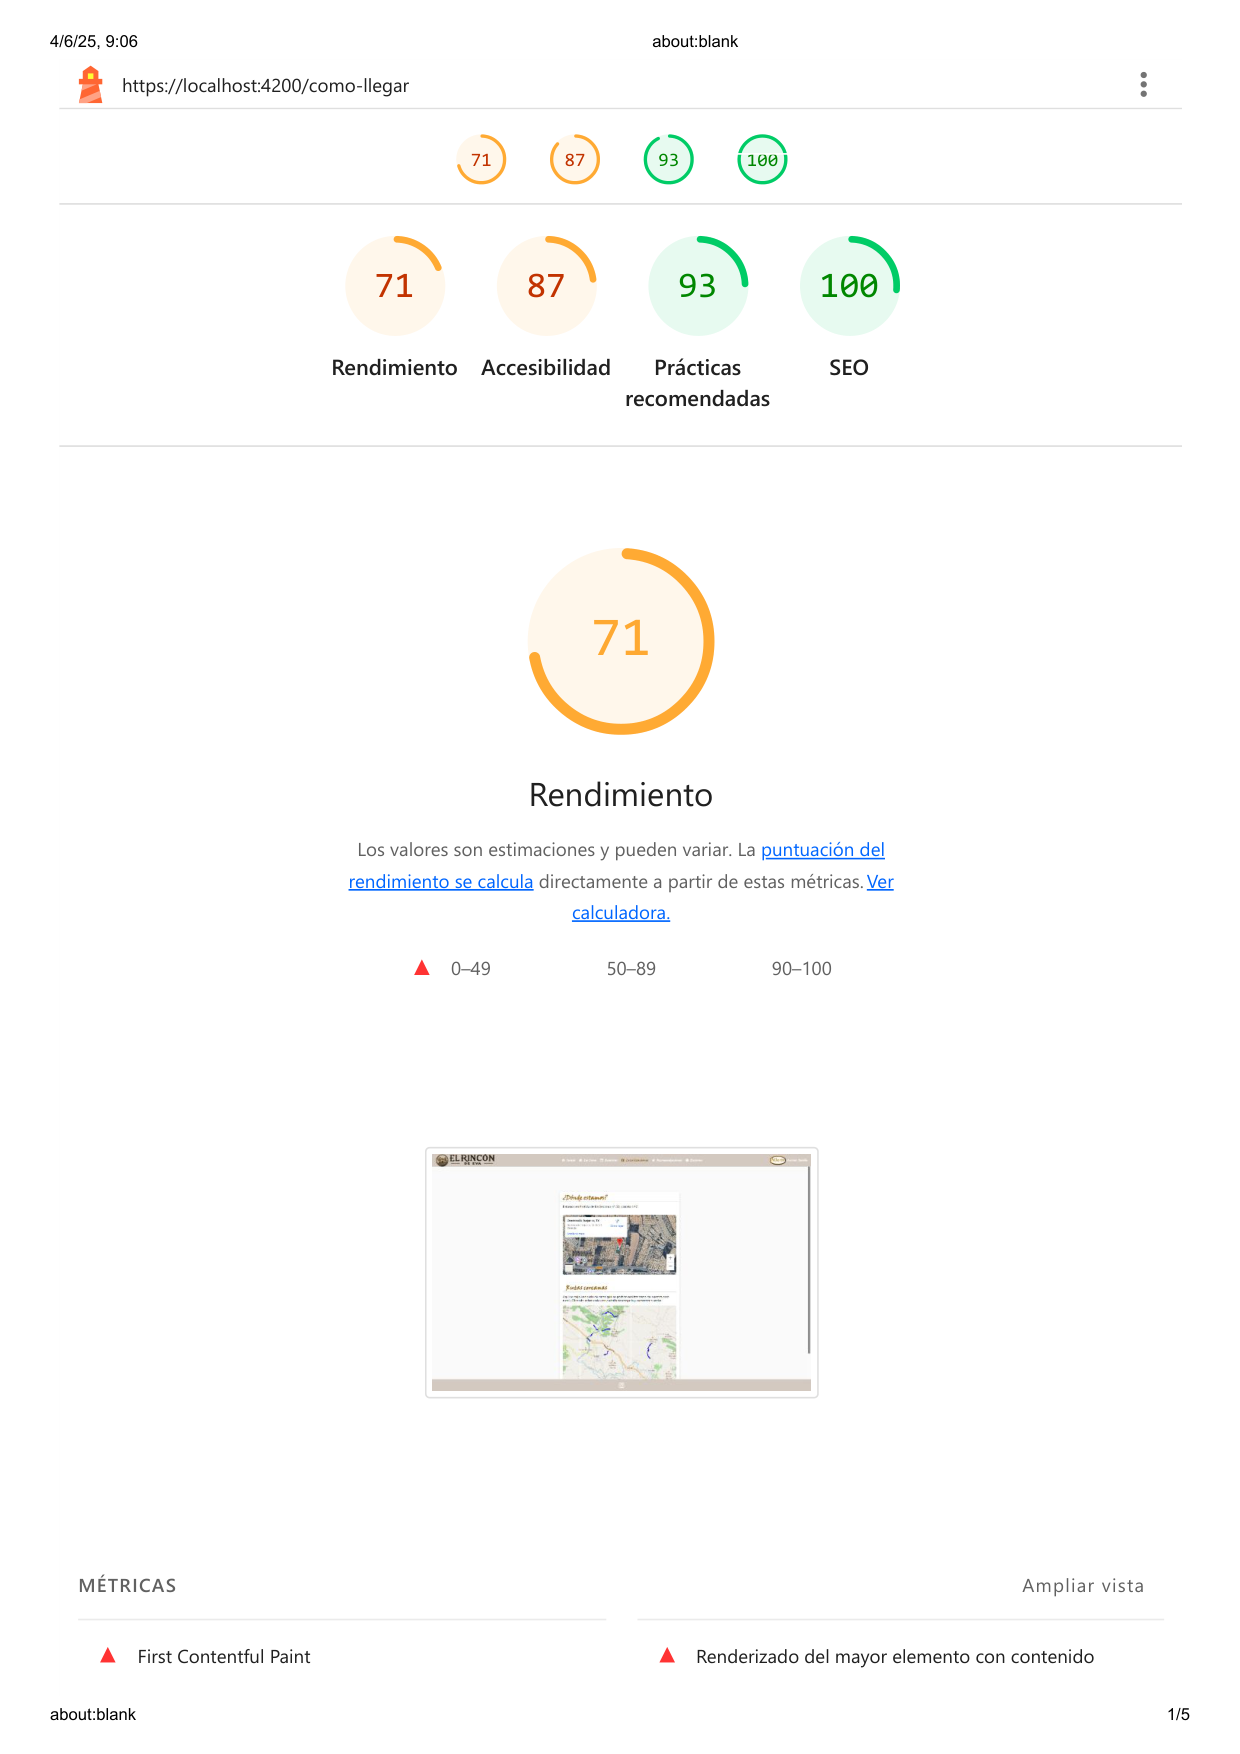
\includegraphics[width=0.85\textwidth]{figs/localizaciones_lighthouse.png}
  \caption{Resultados Lighthouse — Página de localizaciones}
  \label{fig:lighthouse-localizaciones}
\end{figure}

Esta página obtiene un 87 en accesibilidad y un 93 en prácticas recomendadas. El rendimiento alcanza un 71, con buena respuesta inicial pero presencia de tareas largas y recursos que bloquean el renderizado. Mejorar la compresión de texto, reducir el uso de librerías pesadas y controlar los cambios de diseño puede incrementar la puntuación.

\subsection*{Página de recomendaciones}

\begin{figure}[h!tb]
  \centering
  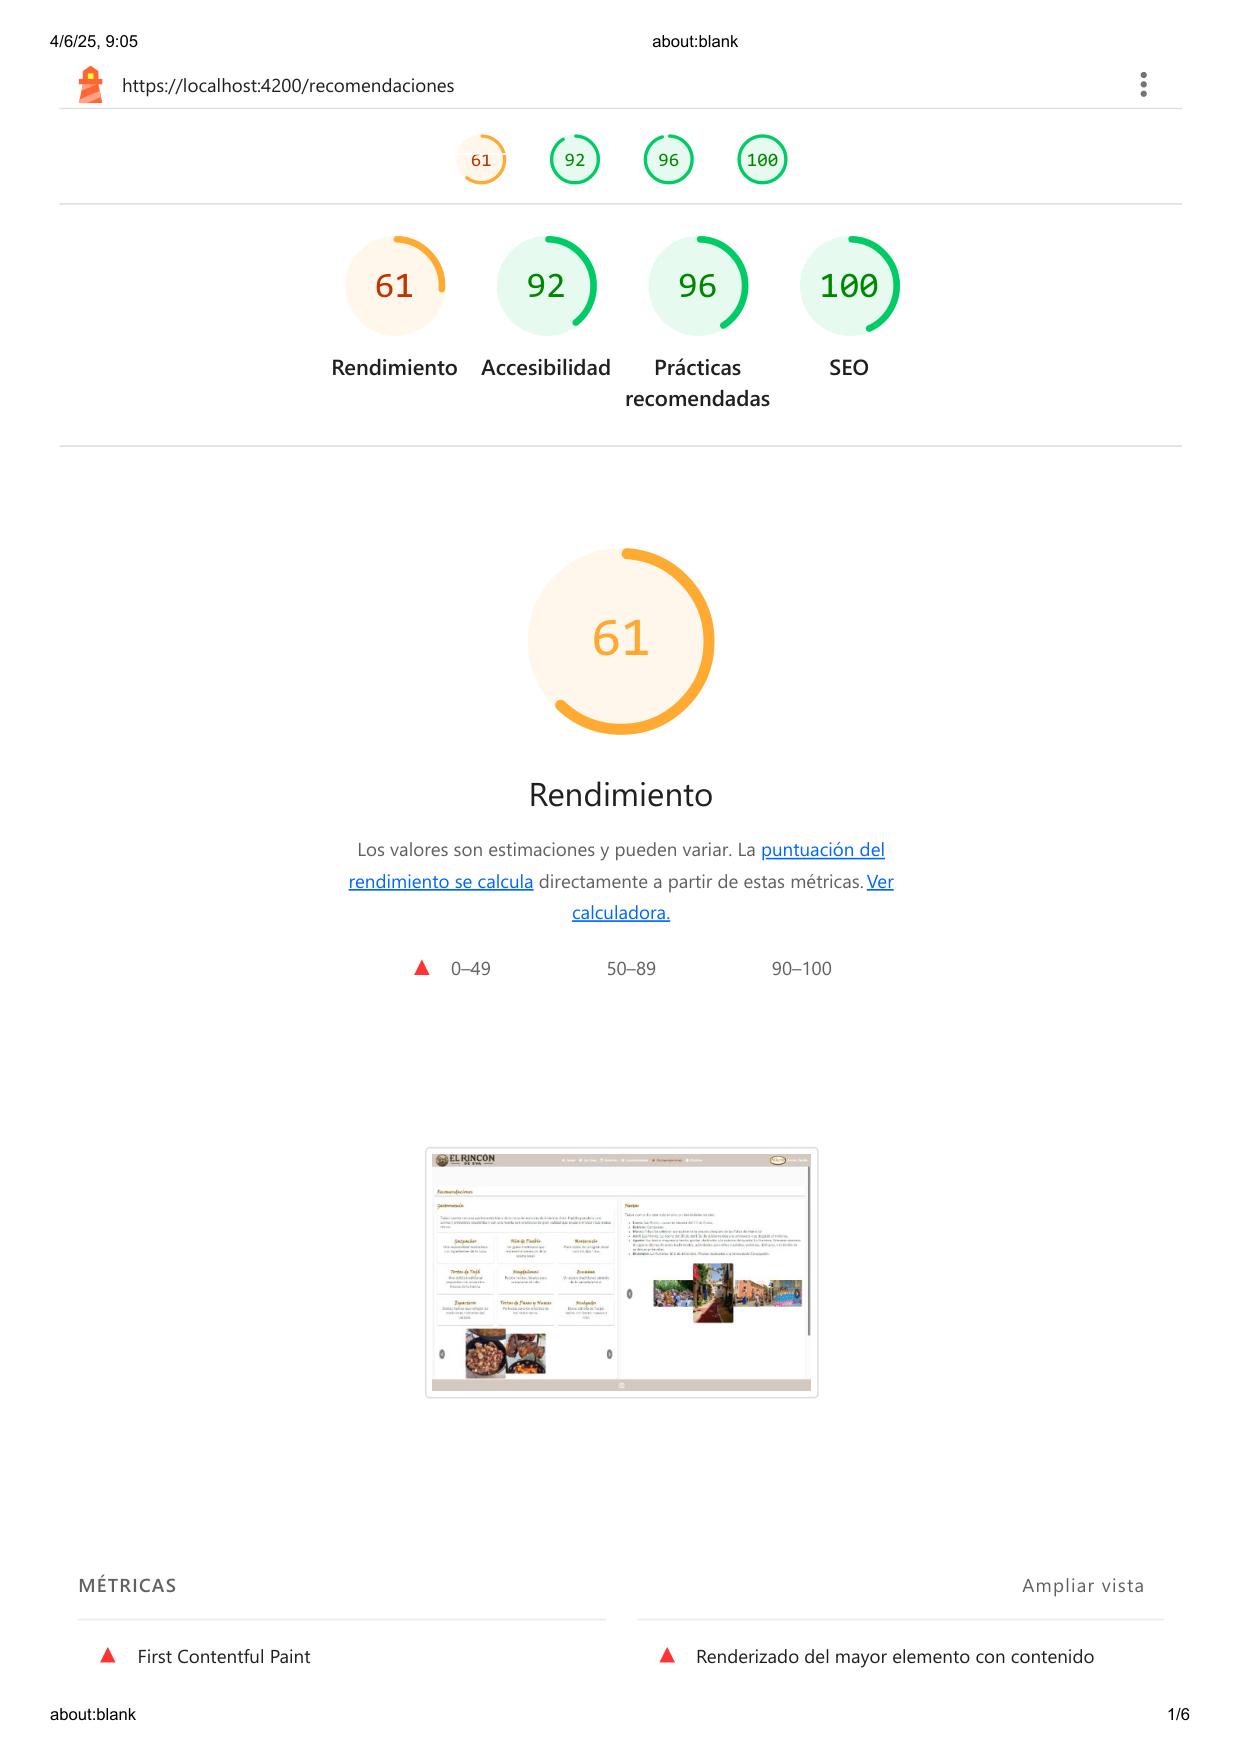
\includegraphics[width=0.85\textwidth]{figs/recomendaciones_lighthouse.png}
  \caption{Resultados Lighthouse — Página de recomendaciones}
  \label{fig:lighthouse-recomendaciones}
\end{figure}

Aunque destaca en accesibilidad (92) y \gls{seo} (100), el rendimiento global es bajo (61). Se identifican problemas relacionados con el renderizado de imágenes, animaciones y encadenamiento de solicitudes. También se recomienda reducir el tamaño de las cargas útiles y mejorar el uso de caché.

\subsection*{Página de reservas}

\begin{figure}[h!tb]
  \centering
  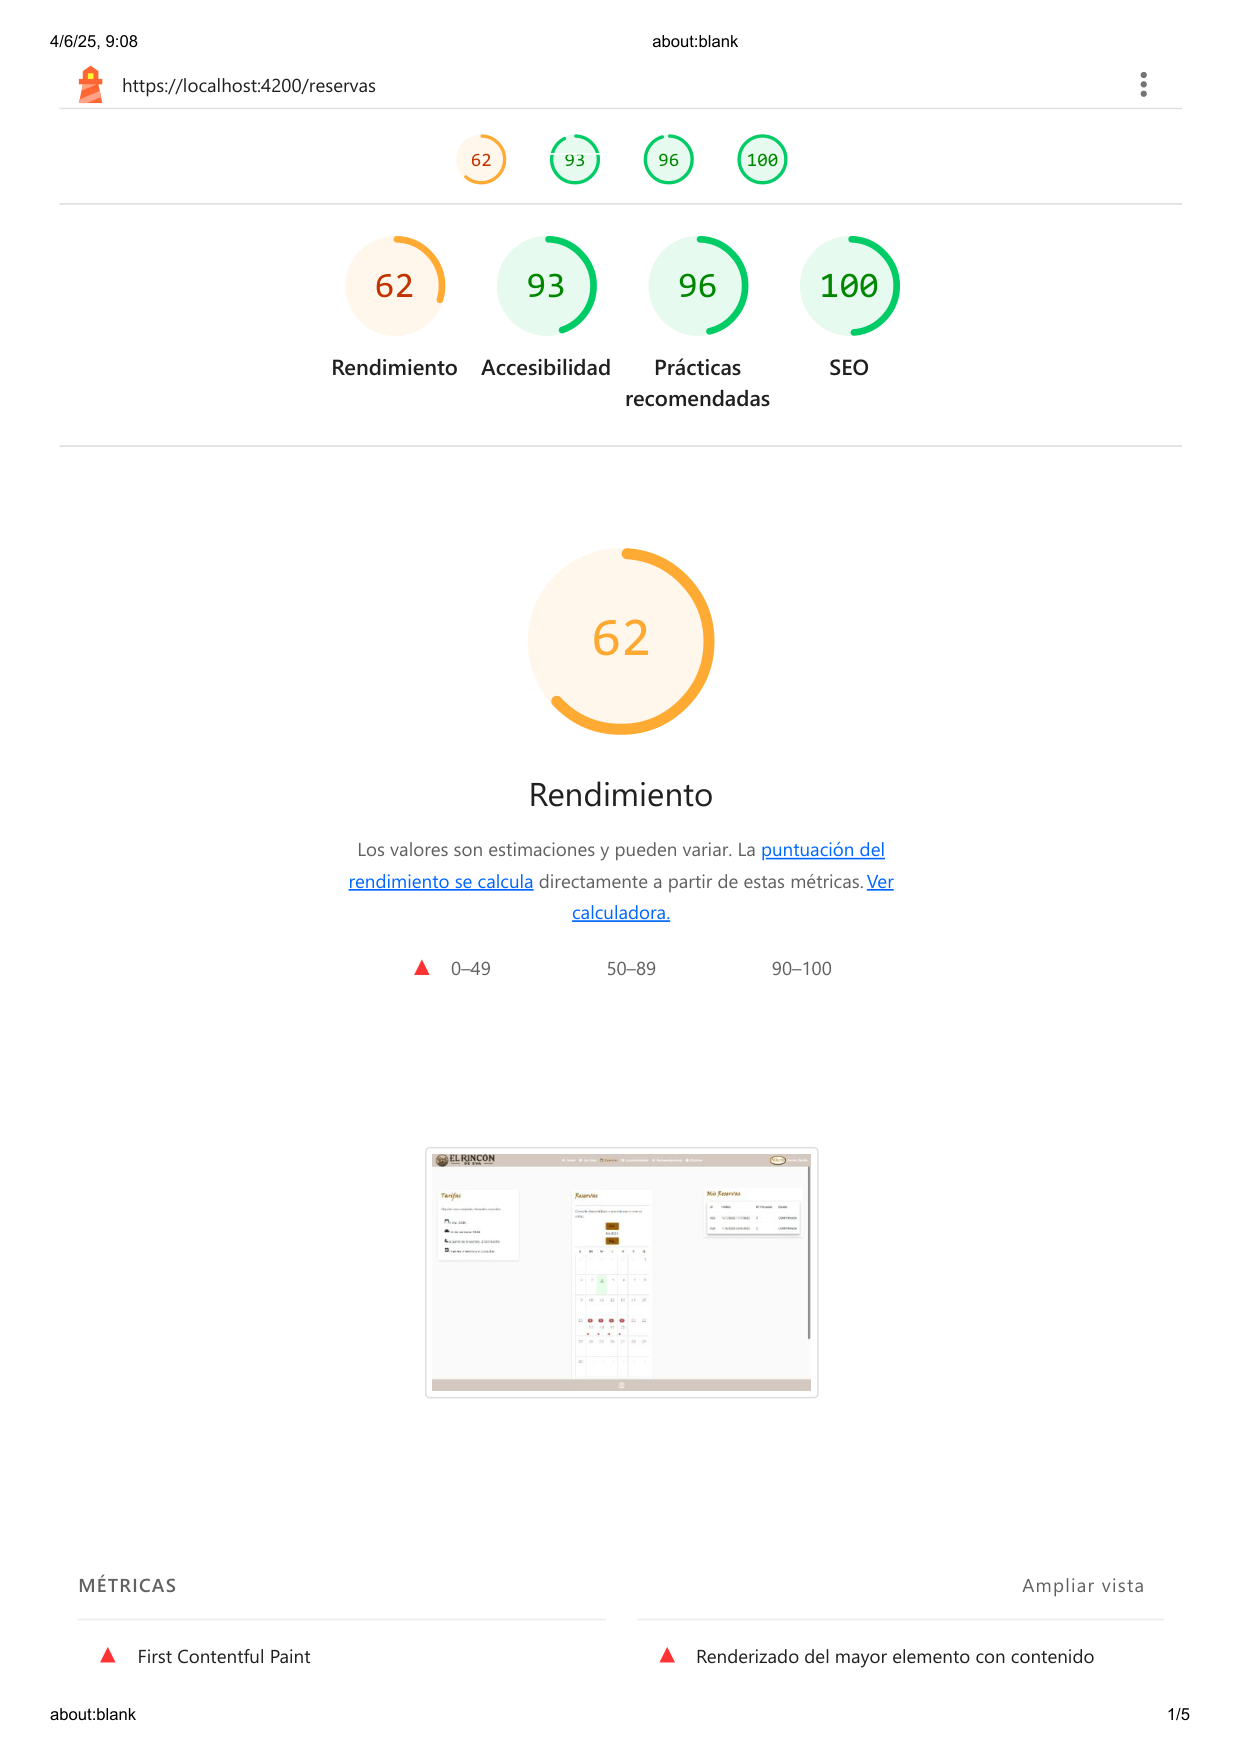
\includegraphics[width=0.85\textwidth]{figs/reservas_lighthouse.png}
  \caption{Resultados Lighthouse — Página de reservas}
  \label{fig:lighthouse-reservas}
\end{figure}

La página de reservas obtiene una puntuación de 93 en accesibilidad, 100 en \gls{seo} y 96 en buenas prácticas. No obstante, el rendimiento es limitado (62) debido a cambios de diseño acumulados y bloqueo del hilo principal. Se sugiere revisar las tareas largas y evitar imágenes sin compresión adecuada.

\subsection*{Conclusiones}

En términos generales, todas las páginas analizadas presentan una \textbf{excelente puntuación en \gls{seo} (100)} y \textbf{muy buena accesibilidad (>86)}, con oportunidades de mejora principalmente en el área de rendimiento. Las recomendaciones comunes incluyen:

\begin{itemize}
    \item Optimizar y precargar imágenes clave.
    \item Reducir \gls{css} y \gls{javascript} no utilizados.
    \item Eliminar recursos que bloqueen el renderizado.
    \item Aplicar formatos modernos y mejorar la caché de recursos.
\end{itemize}

Estas acciones quedan planteadas como línea de trabajo futuro para incrementar la eficiencia y la experiencia de usuario del sitio web.